%%%%%%%%%%%%%%%%%%%%%%%%%%%%%%%%%%%%%%%%%%%%%%%%%%%%%%%%%%%%
% UNCOMMENT THE LINE BELOW TO VIEW COMMENTS
% \def\DraftVersion {}
%%%%%%%%%%%%%%%%%%%%%%%%%%%%%%%%%%%%%%%%%%%%%%%%%%%%%%%%%%%%

% TITLE TO BE PRINTED ON THE HEADERS
\newcommand{\titleOnHeader}{\textsf{IMITATOR} user manual}

% TITLE TO BE PRINTED ON THE FIRST PAGE
\newcommand{\titleOnFirstPage}{IMITATOR User Manual}

\documentclass[a4paper,11pt]{report}

% \sloppy

%%%%%%%%%%%%%%%%%%%%%%%%%%%%%%%%%%%%%%%%%%%%%%%%%%%%%%%%%%%%
% PACKAGES
%%%%%%%%%%%%%%%%%%%%%%%%%%%%%%%%%%%%%%%%%%%%%%%%%%%%%%%%%%%%
\usepackage[utf8]{inputenc}

\usepackage[english]{babel} % francais,
\usepackage{csquotes}

\usepackage{multicol}

\usepackage{fourier}
% \usepackage{eulervm}
% NOTE: both fourier + eulervm make '<' and '>' not displaid!

\usepackage{pdflscape}

\usepackage{amsmath,amssymb,amsthm,url}
\usepackage{amsfonts}

\usepackage{subcaption}
% \usepackage{marginnote}

\usepackage{longtable}

% \usepackage[pdftex]{graphicx,color}
\usepackage[pdftex,
		colorlinks=true,
% 		pagebackref=true,
		citecolor=darkgreen,
		linkcolor=darkblue,
		urlcolor=URLCOLOR,
	]{hyperref}

\usepackage{graphicx}
\graphicspath{{./images/}{../logos/}}


% BEGIN Watermarking
\ifdefined\DraftVersion
	\usepackage{draftwatermark}
	\SetWatermarkText{draft}
	\SetWatermarkScale{2}
	\SetWatermarkColor[gray]{0.9}
\fi
% END Watermarking


\setcounter{secnumdepth}{3}

%%%%%%%%%%%%%%%%%%%%%%%%%%%%%%%%%%%%%%%%%%%%%%%%%%%%%%%%%%%%
% MARGINS, HEADERS AND FOOTERS
%%%%%%%%%%%%%%%%%%%%%%%%%%%%%%%%%%%%%%%%%%%%%%%%%%%%%%%%%%%%

\usepackage[top=1cm,bottom=2.5cm,includeheadfoot,headheight=2.5cm,\ifdefined\DraftVersion showframe \else\fi]{geometry}

% \setlength{\parskip}{1ex}

\usepackage{fancyhdr}
\pagestyle{fancy}

% Reset headers and footers
% \fancyhf{}

% Reset header but not footer
\fancyhead{}

\fancyhead[l]{%
	\titleOnHeader{}
}

\fancyhead[r]{%
	\includegraphics[height=1em]{../logos/imitator-500.png}
	\includegraphics[height=1em]{../logos/logo-3-300.png}
	\includegraphics[height=1em]{../logos/logo-3-4-300.png}
}

\renewcommand{\headrulewidth}{.1pt}
\renewcommand{\footrulewidth}{0pt}

% \fancyfoot[c]{}
% \fancyfoot[R]{\footnotesize{\thepage}}



%%%%%%%%%%%%%%%%%%%%%%%%%%%%%%%%%%%%%%%%%%%%%%%%%%%%%%%%%%%%
% TIKZ
%%%%%%%%%%%%%%%%%%%%%%%%%%%%%%%%%%%%%%%%%%%%%%%%%%%%%%%%%%%%
\usepackage[svgnames,table]{xcolor}

\usepackage{pgf}
\usepackage{tikz}
\usetikzlibrary{arrows,automata,decorations.pathmorphing}
% Couleurs

\definecolor{darkblue}{rgb}{0.0,0.0,0.6}
\definecolor{darkgreen}{rgb}{0, 0.5, 0}
\definecolor{URLCOLOR}{rgb}{.4, .4, .7}


\definecolor{turquoise}{rgb}{0 0.41 0.41}
\definecolor{rouge}{rgb}{0.79 0.0 0.1}
\definecolor{vert}{rgb}{0.15 0.4 0.1}
\definecolor{mauve}{rgb}{0.6 0.4 0.8}
\definecolor{violet}{rgb}{0.58 0. 0.41}
\definecolor{orange}{rgb}{0.8 0.4 0.2}
\definecolor{bleu}{rgb}{0.39, 0.58, 0.93}
\definecolor{gris}{rgb}{0.6,0.6,0.6}
\definecolor{grisfonce}{rgb}{0.4,0.4,0.4}
% Jeu de couleurs pales
\definecolor{cpale1}{rgb}{1, 0.3, 0.3}
\definecolor{cpale2}{rgb}{0.3, 1, 0.3}
\definecolor{cpale3}{rgb}{0.3, 0.3, 1}
\definecolor{cpale4}{rgb}{1, 0.3, 1}
\definecolor{cpale5}{rgb}{1, 1, 0.3}
\definecolor{cpale6}{rgb}{0.3, 1, 1}
\definecolor{cpale7}{rgb}{0.9, 0.6, 0.2}
\definecolor{cpale8}{rgb}{0.7, 0.4, 1}
\definecolor{cpale9}{rgb}{0.5, 1, 0.75}
\definecolor{cpale10}{rgb}{0.8, 0.7, 0.6}
\definecolor{cpale11}{rgb}{0.6, 0.7, 0.8}
\definecolor{cpale12}{rgb}{0.2, 0.5, 0.9}
\definecolor{cpale13}{rgb}{0.5, 0.9, 0.2}
\definecolor{cpale14}{rgb}{0.9, 0.2, 0.5}
\definecolor{cpale15}{rgb}{0.7, 0.7, 0.7}
\definecolor{cpale16}{rgb}{0.8, 0.8, 0.5}


%%%%%%%%%%%%%%%%%%%%%%%%%%%%%%%%%%%%%%%%%%%%%%%%%%%%%%%%%%%%
% CLEVER REFERENCES
%%%%%%%%%%%%%%%%%%%%%%%%%%%%%%%%%%%%%%%%%%%%%%%%%%%%%%%%%%%%
\usepackage[capitalise,english,nameinlink]{cleveref} % load after algorithm2e and hyperref
% \crefname{line}{\text{line}}{\text{lines}} % to remove the capital


%%%%%%%%%%%%%%%%%%%%%%%%%%%%%%%%%%%%%%%%%%%%%%%%%%%%%%%%%%%%
% CONSTANTS
%%%%%%%%%%%%%%%%%%%%%%%%%%%%%%%%%%%%%%%%%%%%%%%%%%%%%%%%%%%%
%-%-%-%-%-%-%-%-%-%-%-%-%-%-%-%-%-%-%-%-%-%-%-%-%-%-%-%-%-%
% MATHS
%-%-%-%-%-%-%-%-%-%-%-%-%-%-%-%-%-%-%-%-%-%-%-%-%-%-%-%-%-%
% Variables
\def\init{\ensuremath{\textsf{init}}} % \xspace
\newcommand{\A}{\mathcal{A}}
\newcommand{\Action}{\ensuremath{\Sigma}}
\newcommand{\action}{a}
\newcommand{\ArithExpr}{\mathcal{AE}} % (#1)% set of all constraints over some set
\newcommand{\ArithExprD}{\ArithExpr(\DVar)}
\newcommand{\ArithExprR}{\ArithExpr(\RVar)}
\newcommand{\ArithExprI}{\ArithExpr(\IVar)}
\newcommand{\ArithExprB}{\ArithExpr(\BVar)}
\newcommand{\ArithExprW}{\ArithExpr(\WVar)}
% \newcommand{\ArithExprA}{\ArithExpr(\AVar)}
\newcommand{\C}{C}
\newcommand{\Cinit}{\C_\init} % initial constraint
\newcommand{\Clock}{X} % set of clocks
\newcommand{\ClockCard}{H} % cardinality of clocks
\newcommand{\clock}{x} % clock
\newcommand{\clockval}{w} % clock valuation
\newcommand{\Cupdates}{\Clock_\mathsf{up}}
\newcommand{\Dupdates}{\DVar_\mathsf{up}}
\newcommand{\dval}{\ensuremath{\delta}} % discrete variable
\newcommand{\DVar}{D} % set of discrete variables
\newcommand{\dvar}{d} % discrete variable
\newcommand{\DVarCard}{J} % cardinality of discrete variables
\newcommand{\rval}{\ensuremath{\rho}} % rational variable
\newcommand{\RVar}{R} % set of rational variables
\newcommand{\rvar}{r} % rational variable
\newcommand{\RVarCard}{J} % cardinality of rational variables
\newcommand{\ival}{\ensuremath{\i}} % integer variable
\newcommand{\IVar}{I} % set of integer variables
\newcommand{\ivar}{i} % integer variable
\newcommand{\IVarCard}{K} % cardinality of integer variables
\newcommand{\bval}{\ensuremath{\beta}} % boolean variable
\newcommand{\BVar}{B} % set of boolean variables
\newcommand{\bvar}{b} % boolean variable
\newcommand{\BVarCard}{L} % cardinality of boolean variables
% \newcommand{\wval}{\ensuremath{\omega}} % binary variable
\newcommand{\WVar}{W} % set of binary word variables
\newcommand{\wvar}{w} % binary word variable % TODO: conflict
% \newcommand{\WVarCard}{M} % cardinality of binary word variables  % TODO: conflict

% \newcommand{\aval}{\ensuremath{\alpha}} % array variable
% \newcommand{\AVar}{A} % set of array variables
% \newcommand{\ElVar}{El} % set of element of array variables
% \newcommand{\avar}{t} % array variable
% \newcommand{\AVarCard}{N} % cardinality of array variables

% Operations
\newcommand{\valuate}[2]{\ensuremath{#2(#1)}}

% \newcommand{\DVarinit}{\DVar_\init} % discrete variable
\newcommand{\edge}{e}
\newcommand{\flow}{\ensuremath{\mathit{flow}}}
\newcommand{\guard}{g}
\newcommand{\invariant}{I}
\newcommand{\LConstraint}{\mathcal{LC}} % (#1)% set of all constraints over some set
\newcommand{\LConstraintD}{\LConstraint(\RVar)}
\newcommand{\LConstraintXP}{\LConstraint(\Clock \cup \Param)}
\newcommand{\LConstraintXPD}{\LConstraint(\Clock \cup \Param \cup \RVar)}
\newcommand{\lterm}{\mathit{lt}}
\newcommand{\LTerm}{\mathcal{LT}} % (#1)% set of all linear terms over some set
\newcommand{\LTermR}{\LTerm(\RVar)}
\newcommand{\LTermXPD}{\LTerm(\Clock \cup \Param \cup \RVar)}
\newcommand{\loc}{\ell} % location
\newcommand{\locinit}{\loc_\init}
\newcommand{\Loc}{L} % set of locations
\newcommand{\Param}{P} % set of parameters
\newcommand{\param}{p} % parameter
\newcommand{\ParamCard}{M} % number of parameters
\newcommand{\pval}{v} % parameter valuation
% \newcommand{\resets}{R}
\newcommand{\steps}{ {\rightarrow} }
% \newcommand{\stopwatches}{\mathit{SW}}
\newcommand{\tuple}[1]{\langle#1\rangle}
\newcommand{\unobs}{\ensuremath{\epsilon}}
\newcommand{\Var}{\mathit{Var}} % set of variables
\newcommand{\var}{\mathit{z}} % variable
\newcommand{\VarCard}{N} % cardinality of variables % TODO: conflict

% Sets
\newcommand{\setA}{\ensuremath{\mathbb A}}
\newcommand{\setB}{\ensuremath{\mathbb B}}
% \newcommand{\setW}{\ensuremath{\mathbb W}}
\newcommand{\setN}{\ensuremath{\mathbb N}}
\newcommand{\setQ}{\ensuremath{\mathbb Q}}
\newcommand{\setQplus}{\ensuremath{\mathbb Q}_{\geq 0}}
\newcommand{\setR}{\ensuremath{\mathbb R}}
\newcommand{\setRplus}{\ensuremath{\setR_{\geq 0}}}
\newcommand{\setZ}{\ensuremath{\mathbb Z}}

\newcommand{\BFalse}{\ensuremath{\mathbf{false}}}
\newcommand{\BTrue}{\ensuremath{\mathbf{true}}}

% Units
\newcommand{\micros}{\mathit{\mu s}}
\newcommand{\nanos}{ns}

% Noms
\newcommand{\pio}{\pi_0}

% Symbols
\newcommand{\emptystring}{\ensuremath{\epsilon}}
\newcommand{\fleche}[1]{\stackrel{#1}{\rightarrow}}
\newcommand{\Fleche}[1]{\stackrel{#1}{\Rightarrow}}
% \newcommand{\steps}[0]{ {\rightarrow} }


%-%-%-%-%-%-%-%-%-%-%-%-%-%-%-%-%-%-%-%-%-%-%-%-%-%-%-%-%-%
% ALGORITHMES
%-%-%-%-%-%-%-%-%-%-%-%-%-%-%-%-%-%-%-%-%-%-%-%-%-%-%-%-%-%
% Algorithmes PTA
\newcommand{\BC}{\ensuremath{\mathsf{BC}}}
\newcommand{\EFsynth}{\ensuremath{\mathsf{EFsynth}}}
\newcommand{\IM}{\ensuremath{\mathsf{IM}}}
\newcommand{\PDFC}{\ensuremath{\mathsf{PDFC}}}
\newcommand{\PRP}{\ensuremath{\mathsf{PRP}}}
\newcommand{\PRPC}{\ensuremath{\mathsf{PRPC}}}


%-%-%-%-%-%-%-%-%-%-%-%-%-%-%-%-%-%-%-%-%-%-%-%-%-%-%-%-%-%
% CONSTANTES DE CHAINES
%-%-%-%-%-%-%-%-%-%-%-%-%-%-%-%-%-%-%-%-%-%-%-%-%-%-%-%-%-%

% Outils
% \newcommand{\apron}{\textsc{Apron}}
\newcommand{\CosyVerif}{\emph{CosyVerif}}
\newcommand{\gdot}{\texttt{dot}}
\newcommand{\graphviz}{Graphviz}
\newcommand{\hytech}{{\sc HyTech}}
\newcommand{\imitator}{\textsf{IMITATOR}}
\newcommand{\imitatorExec}{\code{imitator}}
\newcommand{\IPTA}{IPTA}
\newcommand{\NIPTA}{NIPTA}
\newcommand{\ocaml}{OCaml}
\newcommand{\pat}{PAT}
\newcommand{\phaver}{PHAVer}
\newcommand{\phaverLite}{PHAVerLite}
% \newcommand{\polka}{NewPolka}
% \newcommand{\prism}{\textsc{Prism}}
% \newcommand{\red}{RED}
\newcommand{\uppaal}{\textsc{Uppaal}}
% \newcommand{\jani}{\textsc{The Jani Specification}}
\newcommand{\jani}{\textsc{Jani}}

\newcommand{\binimitator}{./imitator}


% Current version
\newcommand{\imitatorversion}{3.4-beta}
\newcommand{\imitatorversionname}{Cheese Durian}


%%%%%%%%%%%%%%%%%%%%%%%%%%%%%%%%%%%%%%%%%%%%%%%%%%%%%%%%%%%%
% THEOREMS
%%%%%%%%%%%%%%%%%%%%%%%%%%%%%%%%%%%%%%%%%%%%%%%%%%%%%%%%%%%%
\usepackage[framemethod=TikZ]{mdframed}

%------------------------------------------------------------
\theoremstyle{plain}
%------------------------------------------------------------


%------------------------------------------------------------
\theoremstyle{definition}
%------------------------------------------------------------
\newtheorem{mydefinition}{Definition}[chapter]
\newenvironment{definition}%
	{\begin{mdframed}[roundcorner=3pt,backgroundcolor=blue!7,linecolor=blue!70,linewidth=2]\begin{mydefinition}}
	{\end{mydefinition}\end{mdframed}}

\newtheorem{myexample}{Example}[chapter]
\newenvironment{example}
	{\begin{mdframed}[roundcorner=3pt,backgroundcolor=green!7,linecolor=green!70,linewidth=2]\begin{myexample}}
	{\end{myexample}\end{mdframed}}

%------------------------------------------------------------
\theoremstyle{remark}
%------------------------------------------------------------
\newtheorem{myremark}{Remark}[chapter]
\newenvironment{remark}
	{\begin{mdframed}[roundcorner=3pt,backgroundcolor=pink!7,linecolor=pink!70,linewidth=2]\begin{myremark}}
	{\end{myremark}\end{mdframed}}

\newtheorem{myhint}{Hint}[chapter]
\newenvironment{hint}
	{\begin{mdframed}[roundcorner=3pt,backgroundcolor=green!7,linecolor=green!70!black,linewidth=2]\begin{myhint}}
	{\end{myhint}\end{mdframed}}

\newtheorem{mywarning}{Warning} %[chapter]
\newenvironment{becareful}
	{\begin{mdframed}[roundcorner=3pt,backgroundcolor=red!20,linecolor=red!50!black,linewidth=2]\begin{mywarning}}
	{\end{mywarning}\end{mdframed}}

\newtheorem{myalias}{Syntax freedom} %[chapter]
\newenvironment{syntaxalias}
	{\begin{mdframed}[roundcorner=3pt,backgroundcolor=green!20,linecolor=green!50!black,linewidth=2]\begin{myalias}\small}
	{\end{myalias}\end{mdframed}}



%%%%%%%%%%%%%%%%%%%%%%%%%%%%%%%%%%%%%%%%%%%%%%%%%%%%%%%%%%%%
% FORMATING
%%%%%%%%%%%%%%%%%%%%%%%%%%%%%%%%%%%%%%%%%%%%%%%%%%%%%%%%%%%%

\hyphenation{IMITATOR}
\hyphenation{Uppaal}

% \newcommand{\paragraphe}[1]{\paragraph{#1.}}

% Non terminal in a grammar
\newcommand{\nt}[1]{$\langle$\emph{#1}$\rangle$}
% Rule name in a grammar
\newcommand{\regleGrammaire}[1]{\bigskip \noindent \nt{#1} :: \\}
% Not taken into account in the grammar
% \newcommand{\npec}[1]{\textcolor{green!50!black}{#1}}
\newcommand{\commentgrammar}[1]{\textcolor{black!50}{\texttt{/* #1 */}}}

\newcommand{\probleme}[2]{
	\medskip
	\noindent
	\fbox{
		\begin{minipage}{0.95\textwidth}
		\textbf{#1}

		#2
		\end{minipage}
	}

	\medskip
}

% \newcommand{\warningbox}[2]{
% 	\medskip
% 	\noindent
% 	\fcolorbox{red!50!black}{red!20}{
% 		\begin{minipage}{0.95\textwidth}
% 		\textbf{Warning: #1}
%
% 		#2
% 		\end{minipage}
% 	}
%
% 	\medskip
% }

% \newcommand{\commentaire}[1]{\textcolor{red}{\textbf{$\Leftarrow$  #1 $\Rightarrow$}}} % commentaire dans un paragraphe
% \newcommand{\commentaire}[1]{}


% Code integre au texte
% \newcommand{\code}[1]{\textbf{\texttt{#1}}}


\definecolor{imicolor}{rgb}{0, .4, .4}
\newcommand{\styleIMI}[1]{\textcolor{imicolor}{\texttt{#1}}}

\definecolor{optioncolor}{rgb}{.4, 0, .4}
\newcommand{\styleOption}[1]{\textcolor{optioncolor}{\texttt{#1}}}
\newcommand{\styleOptionValue}[1]{\textcolor{optioncolor}{\texttt{#1}}}

\definecolor{pathcolor}{rgb}{1, .5, 0}
\newcommand{\stylePath}[1]{\textcolor{pathcolor}{\texttt{#1}}}

\definecolor{filecontentcolor}{rgb}{.1, .4, .2}
\newcommand{\styleFileContent}[1]{\textcolor{filecontentcolor}{\texttt{#1}}}

\newcommand{\styleTCTL}[1]{\ensuremath{\mathsf{#1}}}

\newcommand{\GitHubIMI}{\href{https://github.com/imitator-model-checker/imitator}{GitHub}}

% \newcommand{\styleCommand}[1]{
% 	\medskip
% 
% 	% \mbox{}\hspace{.5cm}
% 	\noindent\fcolorbox{white}{black!90}{
% 		\textcolor{yellow!30}{\$\ \ \texttt{#1}}
% 	}
% 
% 	\medskip
% 
% }

% \newcommand{\styleTerminalOutput}[1]{
% 	\medskip
% 
% 	% \mbox{}\hspace{.5cm}
% 	\noindent\fcolorbox{white}{black!90}{
% 	\begin{minipage}{.97\textwidth}
% 		\textcolor{yellow!30}{\texttt{#1}}
% 	\end{minipage}
% 	}
% 
% 	\medskip
% 
% }


%%%%%%%%%%%%%%%%%%%%%%%%%%%%%%%%%%%%%%%%%%%%%%%%%%%%%%%%%%%%
% COLORS AND TABLES
%%%%%%%%%%%%%%%%%%%%%%%%%%%%%%%%%%%%%%%%%%%%%%%%%%%%%%%%%%%%
\newcommand{\cellHeader}[1]{\cellcolor{blue!20}\textbf{#1}}
\newcommand{\rowHeader}{\rowcolor{blue!20}}

\definecolor{vertfonce}{rgb}{0.0, 0.5, 0.0}
\definecolor{rougefonce}{rgb}{1, 0.0, 0.0}
\newcommand{\compyes}{$\textcolor{vertfonce}{\mathbf{\surd}}$}
\newcommand{\compno}{$\textcolor{rougefonce}{\mathbf{\times}}$}

\newcommand{\cellYes}{\cellcolor{green!20}\textbf{\compyes}}
\newcommand{\cellYesNo}{\cellcolor{orange!20}\textbf{\compyes/\compno}}
\newcommand{\cellNo}{\cellcolor{red!20}\textbf{\compno}}
\newcommand{\cellNA}{\cellcolor{black!20}N/A}
\newcommand{\cellUnclear}{\cellcolor{yellow!20}\textbf{?}}

%%%%%%%%%%%%%%%%%%%%%%%%%%%%%%%%%%%%%%%%%%%%%%%%%%%%%%%%%%%%
% I.E. / E.G. / W.R.T.
%%%%%%%%%%%%%%%%%%%%%%%%%%%%%%%%%%%%%%%%%%%%%%%%%%%%%%%%%%%%

% Helps to spot the places where macros are NOT used
\ifdefined \DraftVersion
 	\definecolor{colorok}{RGB}{80,80,150}
\else
	\definecolor{colorok}{RGB}{0,0,0}
\fi

% \newcommand{\eg}{\textcolor{colorok}{\textit{e.g.}}\xspace}
% \newcommand{\ie}{\textcolor{colorok}{\textit{i.e.}}\xspace}
% \newcommand{\wrt}{\textcolor{colorok}{w.r.t.}\xspace}
\newcommand{\adhoc}{\textcolor{colorok}{\textit{ad-hoc}\@}}
\newcommand{\eg}{\textcolor{colorok}{\textit{e.g.},\@}}
\newcommand{\ie}{\textcolor{colorok}{\textit{i.e.},\@}}
\newcommand{\wrt}{\textcolor{colorok}{w.r.t.}\@}





%%%%%%%%%%%%%%%%%%%%%%%%%%%%%%%%%%%%%%%%%%%%%%%%%%%%%%%%%%%%
% IMITATOR FILES
%%%%%%%%%%%%%%%%%%%%%%%%%%%%%%%%%%%%%%%%%%%%%%%%%%%%%%%%%%%%
\definecolor{bggcolor}{rgb}{0.95,0.95,0.95}
\definecolor{commentscolor}{rgb}{0.5,0.5,0.6}
% \definecolor{numberscolor}{rgb}{0.1,.5,0.1}
\definecolor{keywordscolor}{rgb}{0.0, 0.0, 1.0}
\definecolor{numberscolor}{rgb}{0.6, 0.6, 0.6}
% \definecolor{stringscolor}{rgb}{1,0.6,0.6}
\definecolor{binarycolor}{rgb}{1, 0.0, 0.0}


\usepackage{listings}
\newcommand{\IncludeIMIfile}[1]{
	\lstset{style=IMITATORmodel}
	\lstinputlisting[
		basicstyle=\footnotesize,
% 		breaklines=true,
% 		breakatwhitespace=true,
		columns=fixed,
% 		numbers=left,
% 		frame=single,
% 		numberstyle=\tiny,
% 		tabsize=4,
% 		title=\lstname
	]{#1}
}

\newcommand{\IncludeIMIproperty}[1]{
	\lstset{style=IMITATORproperty}
	\lstinputlisting[]{#1}
}

\lstdefinestyle{IMITATORmodel}{
	backgroundcolor=\color{white},   % choose the background color; you must add \usepackage{color} or \usepackage{xcolor}; should come as last argument
	basicstyle=\tt\footnotesize,        % the size of the fonts that are used for the code
	breakatwhitespace=true,         % sets if automatic breaks should only happen at whitespace
	breaklines=true,                 % sets automatic line breaking
	%   captionpos=b,                    % sets the caption-position to bottom
	commentstyle=\color{commentscolor},    % comment style
	escapeinside={\%*}{*)},          % if you want to add LaTeX within your code
	extendedchars=true,              % lets you use non-ASCII characters; for 8-bits encodings only, does not work with UTF-8
	%   firstnumber=1,                % start line enumeration with line 1000
	frame=single,	                   % adds a frame around the code
	keepspaces=true,                 % keeps spaces in text, useful for keeping indentation of code (possibly needs columns=flexible)
	keywordstyle=\bfseries\color{keywordscolor},       % keyword style
	language=caml,                 % the language of the code
	deletekeywords={done},            % if you want to delete keywords from the given language; WARNING! must be set AFTER the `language=…`
	morekeywords={
		accepting, actions, and, array, array_append, array_length, array_mem, automaton,
		begin, binary, bool,
		clock, constant, continuous, controllable,
		discrete, do, done, downto,
		else, end,
		False, fill_left, fill_right, flow, fn, from, function,
		goto,
		if, in, init, initially, int, int_div, inside, invariant, is,
		list, list_cons, list_hd, list_is_empty, list_length, list_mem, list_rev, list_tl, loc, logand, lognot, logor, logxor,
		mod,
		not,
		or,
		parameter, pow,
		queue, queue_clear, queue_is_empty, queue_length, queue_pop, queue_push, queue_top,
		rat, rational, return,
		shift_left, shift_right, stack, stack_clear, stack_is_empty, stack_length, stack_pop, stack_push, stack_top, stop, sync,
		then, to, True,
		urgent,
		var, void,
		when, while,
	},
	numbers=right,                    % where to put the line-numbers; possible values are (none, left, right)
	numbersep=5pt,                   % how far the line-numbers are from the code
	numberstyle=\tiny\color{numberscolor}, % the style that is used for the line-numbers
	rulecolor=\color{black},         % if not set, the frame-color may be changed on line-breaks within not-black text (e.g. comments (green here))
	showspaces=false,                % show spaces everywhere adding particular underscores; it overrides 'showstringspaces'
	showstringspaces=false,          % underline spaces within strings only
	showtabs=false,                  % show tabs within strings adding particular underscores
	stepnumber=1,                    % the step between two line-numbers. If it's 1, each line will be numbered
% 	stringstyle=\color{stringscolor},     % string literal style
	tabsize=2,	                   % sets default tabsize to 2 spaces
	sensitive=false,
% 	morecomment=[l][\color{gray}]{--},
% 	morecomment=[s][keywordstyle]{"}{"},
% 	morecomment=[s]{/*}{*/},
% 	morestring=[s][\color{red}]{0b}, % values: b,d,m,s(*2?)
	moredelim=[s][\color{binarycolor}]{0b}{\ },
	moredelim=[s][\color{red}]{\#}{\ },
	morecomment=[s][\color{commentscolor}]{(*}{*)},
		% values: lfdnms
	% For UTF-8
	inputencoding=utf8,
    extendedchars=true,
    literate=
        {á}{{\'a}}1  {é}{{\'e}}1  {í}{{\'i}}1 {ó}{{\'o}}1  {ú}{{\'u}}1
      {Á}{{\'A}}1  {É}{{\'E}}1  {Í}{{\'I}}1 {Ó}{{\'O}}1  {Ú}{{\'U}}1
      {à}{{\`a}}1  {è}{{\`e}}1  {ì}{{\`i}}1 {ò}{{\`o}}1  {ù}{{\`u}}1
      {À}{{\`A}}1  {È}{{\'E}}1  {Ì}{{\`I}}1 {Ò}{{\`O}}1  {Ù}{{\`U}}1
      {ä}{{\"a}}1  {ë}{{\"e}}1  {ï}{{\"i}}1 {ö}{{\"o}}1  {ü}{{\"u}}1
      {Ä}{{\"A}}1  {Ë}{{\"E}}1  {Ï}{{\"I}}1 {Ö}{{\"O}}1  {Ü}{{\"U}}1
      {â}{{\^a}}1  {ê}{{\^e}}1  {î}{{\^i}}1 {ô}{{\^o}}1  {û}{{\^u}}1
      {Â}{{\^A}}1  {Ê}{{\^E}}1  {Î}{{\^I}}1 {Ô}{{\^O}}1  {Û}{{\^U}}1
      {œ}{{\oe}}1  {Œ}{{\OE}}1  {æ}{{\ae}}1 {Æ}{{\AE}}1  {ß}{{\ss}}1
      {ç}{{\c c}}1 {Ç}{{\c C}}1 {ø}{{\o}}1  {Ø}{{\O}}1   {å}{{\r a}}1
      {Å}{{\r A}}1 {ã}{{\~a}}1  {õ}{{\~o}}1 {Ã}{{\~A}}1  {Õ}{{\~O}}1
      {ñ}{{\~n}}1  {Ñ}{{\~N}}1  {¿}{{?`}}1  {¡}{{!`}}1
      {ā}{{\=a}}1  {Ā}{{\=A}}1 {ē}{{\=e}}1  {Ē}{{\=E}}1 {ī}{{\=i}}1 {Ī}{{\=I}}1 {ō}{{\=o}}1 {Ō}{{\=O}}1 {ū}{{\=u}}1 {Ū}{{\=U}}1 
      ,
}



\lstdefinestyle{IMITATORproperty}{
  backgroundcolor=\color{bggcolor},   % choose the background color; you must add \usepackage{color} or \usepackage{xcolor}; should come as last argument
  basicstyle=\tt\scriptsize,        % the size of the fonts that are used for the code
%   breakatwhitespace=false,         % sets if automatic breaks should only happen at whitespace
  breaklines=true,                 % sets automatic line breaking
%   captionpos=b,                    % sets the caption-position to bottom
  commentstyle=\color{commentscolor},    % comment style
%   deletekeywords={},            % if you want to delete keywords from the given language
  escapeinside={\%*}{*)},          % if you want to add LaTeX within your code
  extendedchars=true,              % lets you use non-ASCII characters; for 8-bits encodings only, does not work with UTF-8
%   firstnumber=1000,                % start line enumeration with line 1000
  frame=single,	                   % adds a frame around the code
  keepspaces=true,                 % keeps spaces in text, useful for keeping indentation of code (possibly needs columns=flexible)
  keywordstyle=\bfseries\color{keywordscolor},       % keyword style
%   language=caml,                 % the language of the code
  morekeywords={%
	A, accepting, AF, AF_, AGnot, always,
	BCcover, BCrandom, BCshuffle, before,
	Cycle, CycleThrough,
	DeadlockFree,
	E, EF, EF_, EFpmin, EFpmax, EFtmin, everytime, eventually,
	happened, has,
	IM, infinity,
	loc,
	next,
	once,
	pattern, PRP, PRPC, property,
	R, R_,
	sequence, synth,
	U, U_,
	W, W_, within, witness},            % if you want to add more keywords to the set
  numbers=none,                    % where to put the line-numbers; possible values are (none, left, right)
%   numbersep=5pt,                   % how far the line-numbers are from the code
%   numberstyle=\tiny\color{bggcolor}, % the style that is used for the line-numbers
%   rulecolor=\color{black},         % if not set, the frame-color may be changed on line-breaks within not-black text (e.g. comments (green here))
%   showspaces=false,                % show spaces everywhere adding particular underscores; it overrides 'showstringspaces'
%   showstringspaces=false,          % underline spaces within strings only
%   showtabs=false,                  % show tabs within strings adding particular underscores
%   stepnumber=2,                    % the step between two line-numbers. If it's 1, each line will be numbered
%   stringstyle=\color{stringscolor},     % string literal style
%   tabsize=2,	                   % sets default tabsize to 2 spaces
%   title=\lstname                   % show the filename of files included with \lstinputlisting; also try caption instead of title
	morecomment=[s][\color{commentscolor}]{(*}{*)},
	% For UTF-8
	inputencoding=utf8,
    extendedchars=true,
    literate=
        {á}{{\'a}}1  {é}{{\'e}}1  {í}{{\'i}}1 {ó}{{\'o}}1  {ú}{{\'u}}1
      {Á}{{\'A}}1  {É}{{\'E}}1  {Í}{{\'I}}1 {Ó}{{\'O}}1  {Ú}{{\'U}}1
      {à}{{\`a}}1  {è}{{\`e}}1  {ì}{{\`i}}1 {ò}{{\`o}}1  {ù}{{\`u}}1
      {À}{{\`A}}1  {È}{{\'E}}1  {Ì}{{\`I}}1 {Ò}{{\`O}}1  {Ù}{{\`U}}1
      {ä}{{\"a}}1  {ë}{{\"e}}1  {ï}{{\"i}}1 {ö}{{\"o}}1  {ü}{{\"u}}1
      {Ä}{{\"A}}1  {Ë}{{\"E}}1  {Ï}{{\"I}}1 {Ö}{{\"O}}1  {Ü}{{\"U}}1
      {â}{{\^a}}1  {ê}{{\^e}}1  {î}{{\^i}}1 {ô}{{\^o}}1  {û}{{\^u}}1
      {Â}{{\^A}}1  {Ê}{{\^E}}1  {Î}{{\^I}}1 {Ô}{{\^O}}1  {Û}{{\^U}}1
      {œ}{{\oe}}1  {Œ}{{\OE}}1  {æ}{{\ae}}1 {Æ}{{\AE}}1  {ß}{{\ss}}1
      {ç}{{\c c}}1 {Ç}{{\c C}}1 {ø}{{\o}}1  {Ø}{{\O}}1   {å}{{\r a}}1
      {Å}{{\r A}}1 {ã}{{\~a}}1  {õ}{{\~o}}1 {Ã}{{\~A}}1  {Õ}{{\~O}}1
      {ñ}{{\~n}}1  {Ñ}{{\~N}}1  {¿}{{?`}}1  {¡}{{!`}}1
      {ā}{{\=a}}1  {Ā}{{\=A}}1 {ē}{{\=e}}1  {Ē}{{\=E}}1 {ī}{{\=i}}1 {Ī}{{\=I}}1 {ō}{{\=o}}1 {Ō}{{\=O}}1 {ū}{{\=u}}1 {Ū}{{\=U}}1 
      ,
}


\definecolor{commentscolorterminal}{rgb}{0.6,0.6,0.6}
% \definecolor{numberscolorterminal}{rgb}{0.3,.3,0.3}
\definecolor{stringscolorterminal}{rgb}{.6,1,0.6}

\lstdefinestyle{terminal}{
	backgroundcolor=\color{black},   % choose the background color; you must add \usepackage{color} or \usepackage{xcolor}; should come as last argument
	basicstyle=\ttfamily\small\color{yellow},        % the size of the fonts that are used for the code
	breakatwhitespace=true,         % sets if automatic breaks should only happen at whitespace
	breaklines=true,                 % sets automatic line breaking
	%   captionpos=b,                    % sets the caption-position to bottom
	commentstyle=\color{commentscolorterminal},    % comment style
	escapeinside={\%*}{*)},          % if you want to add LaTeX within your code
	%   firstnumber=1,                % start line enumeration with line 1000
	frame=single,	                   % adds a frame around the code
	keepspaces=true,                 % keeps spaces in text, useful for keeping indentation of code (possibly needs columns=flexible)
	keywordstyle=\bfseries\color{orange},       % keyword style
	language=bash,                 % the language of the code
% 	deletekeywords={done},            % if you want to delete keywords from the given language; WARNING! must be set AFTER the `language=…`
	morekeywords={
		grep, imitator
	},
	numbers=none,                    % where to put the line-numbers; possible values are (none, left, right)
% 	numbersep=5pt,                   % how far the line-numbers are from the code
% 	numberstyle=\tiny\color{numberscolorterminal}, % the style that is used for the line-numbers
	rulecolor=\color{black},         % if not set, the frame-color may be changed on line-breaks within not-black text (e.g. comments (green here))
	showspaces=false,                % show spaces everywhere adding particular underscores; it overrides 'showstringspaces'
	showstringspaces=false,          % underline spaces within strings only
	showtabs=false,                  % show tabs within strings adding particular underscores
	stepnumber=1,                    % the step between two line-numbers. If it's 1, each line will be numbered
	stringstyle=\color{stringscolorterminal},     % string literal style
	tabsize=2,	                   % sets default tabsize to 2 spaces
	sensitive=false,
	% For UTF-8
	inputencoding=utf8,
    extendedchars=true,
    literate=
        {á}{{\'a}}1  {é}{{\'e}}1  {í}{{\'i}}1 {ó}{{\'o}}1  {ú}{{\'u}}1
      {Á}{{\'A}}1  {É}{{\'E}}1  {Í}{{\'I}}1 {Ó}{{\'O}}1  {Ú}{{\'U}}1
      {à}{{\`a}}1  {è}{{\`e}}1  {ì}{{\`i}}1 {ò}{{\`o}}1  {ù}{{\`u}}1
      {À}{{\`A}}1  {È}{{\'E}}1  {Ì}{{\`I}}1 {Ò}{{\`O}}1  {Ù}{{\`U}}1
      {ä}{{\"a}}1  {ë}{{\"e}}1  {ï}{{\"i}}1 {ö}{{\"o}}1  {ü}{{\"u}}1
      {Ä}{{\"A}}1  {Ë}{{\"E}}1  {Ï}{{\"I}}1 {Ö}{{\"O}}1  {Ü}{{\"U}}1
      {â}{{\^a}}1  {ê}{{\^e}}1  {î}{{\^i}}1 {ô}{{\^o}}1  {û}{{\^u}}1
      {Â}{{\^A}}1  {Ê}{{\^E}}1  {Î}{{\^I}}1 {Ô}{{\^O}}1  {Û}{{\^U}}1
      {œ}{{\oe}}1  {Œ}{{\OE}}1  {æ}{{\ae}}1 {Æ}{{\AE}}1  {ß}{{\ss}}1
      {ç}{{\c c}}1 {Ç}{{\c C}}1 {ø}{{\o}}1  {Ø}{{\O}}1   {å}{{\r a}}1
      {Å}{{\r A}}1 {ã}{{\~a}}1  {õ}{{\~o}}1 {Ã}{{\~A}}1  {Õ}{{\~O}}1
      {ñ}{{\~n}}1  {Ñ}{{\~N}}1  {¿}{{?`}}1  {¡}{{!`}}1
      {ā}{{\=a}}1  {Ā}{{\=A}}1 {ē}{{\=e}}1  {Ē}{{\=E}}1 {ī}{{\=i}}1 {Ī}{{\=I}}1 {ō}{{\=o}}1 {Ō}{{\=O}}1 {ū}{{\=u}}1 {Ū}{{\=U}}1 
    ,
}

% Define empty language
\lstdefinelanguage{none}{
  identifierstyle=
}

\lstdefinestyle{terminaloutput}{
	backgroundcolor=\color{black},   % choose the background color; you must add \usepackage{color} or \usepackage{xcolor}; should come as last argument
	basicstyle=\ttfamily\small\color{yellow},        % the size of the fonts that are used for the code
	breakatwhitespace=true,         % sets if automatic breaks should only happen at whitespace
	breaklines=true,                 % sets automatic line breaking
	%   captionpos=b,                    % sets the caption-position to bottom
	commentstyle=\color{commentscolorterminal},    % comment style
	escapeinside={\%*}{*)},          % if you want to add LaTeX within your code
	extendedchars=true,              % lets you use non-ASCII characters; for 8-bits encodings only, does not work with UTF-8
	%   firstnumber=1,                % start line enumeration with line 1000
	frame=single,	                   % adds a frame around the code
	keepspaces=true,                 % keeps spaces in text, useful for keeping indentation of code (possibly needs columns=flexible)
% 	keywordstyle=\bfseries\color{orange},       % keyword style
	language=none,                 % the language of the code
% 	deletekeywords={done},            % if you want to delete keywords from the given language; WARNING! must be set AFTER the `language=…`
% 	morekeywords={
% 		imitator
% 	},
	numbers=none,                    % where to put the line-numbers; possible values are (none, left, right)
% 	numbersep=5pt,                   % how far the line-numbers are from the code
% 	numberstyle=\tiny\color{numberscolorterminal}, % the style that is used for the line-numbers
	rulecolor=\color{black},         % if not set, the frame-color may be changed on line-breaks within not-black text (e.g. comments (green here))
	showspaces=false,                % show spaces everywhere adding particular underscores; it overrides 'showstringspaces'
	showstringspaces=false,          % underline spaces within strings only
	showtabs=false,                  % show tabs within strings adding particular underscores
	stepnumber=1,                    % the step between two line-numbers. If it's 1, each line will be numbered
	stringstyle=\color{stringscolorterminal},     % string literal style
	tabsize=2,	                   % sets default tabsize to 2 spaces
	sensitive=false,
	% For UTF-8
	inputencoding=utf8,
    extendedchars=true,
    literate=
        {á}{{\'a}}1  {é}{{\'e}}1  {í}{{\'i}}1 {ó}{{\'o}}1  {ú}{{\'u}}1
      {Á}{{\'A}}1  {É}{{\'E}}1  {Í}{{\'I}}1 {Ó}{{\'O}}1  {Ú}{{\'U}}1
      {à}{{\`a}}1  {è}{{\`e}}1  {ì}{{\`i}}1 {ò}{{\`o}}1  {ù}{{\`u}}1
      {À}{{\`A}}1  {È}{{\'E}}1  {Ì}{{\`I}}1 {Ò}{{\`O}}1  {Ù}{{\`U}}1
      {ä}{{\"a}}1  {ë}{{\"e}}1  {ï}{{\"i}}1 {ö}{{\"o}}1  {ü}{{\"u}}1
      {Ä}{{\"A}}1  {Ë}{{\"E}}1  {Ï}{{\"I}}1 {Ö}{{\"O}}1  {Ü}{{\"U}}1
      {â}{{\^a}}1  {ê}{{\^e}}1  {î}{{\^i}}1 {ô}{{\^o}}1  {û}{{\^u}}1
      {Â}{{\^A}}1  {Ê}{{\^E}}1  {Î}{{\^I}}1 {Ô}{{\^O}}1  {Û}{{\^U}}1
      {œ}{{\oe}}1  {Œ}{{\OE}}1  {æ}{{\ae}}1 {Æ}{{\AE}}1  {ß}{{\ss}}1
      {ç}{{\c c}}1 {Ç}{{\c C}}1 {ø}{{\o}}1  {Ø}{{\O}}1   {å}{{\r a}}1
      {Å}{{\r A}}1 {ã}{{\~a}}1  {õ}{{\~o}}1 {Ã}{{\~A}}1  {Õ}{{\~O}}1
      {ñ}{{\~n}}1  {Ñ}{{\~N}}1  {¿}{{?`}}1  {¡}{{!`}}1
      {ā}{{\=a}}1  {Ā}{{\=A}}1 {ē}{{\=e}}1  {Ē}{{\=E}}1 {ī}{{\=i}}1 {Ī}{{\=I}}1 {ō}{{\=o}}1 {Ō}{{\=O}}1 {ū}{{\=u}}1 {Ū}{{\=U}}1 
      ,
}

\lstnewenvironment{terminal}[0]
	{%
		\lstset{style=terminal}
	}%
	{}

\lstnewenvironment{terminaloutput}[0]
	{%
		\lstset{style=terminaloutput}
	}%
	{}

\lstnewenvironment{IMITATORmodel}[0]
	{%
		\lstset{style=IMITATORmodel}
	}%
	{}

\lstnewenvironment{IMITATORproperty}[0]
	{%
		\lstset{style=IMITATORproperty}
	}%
	{}


%%%%%%%%%%%%%%%%%%%%%%%%%%%%%%%%%%%%%%%%%%%%%%%%%%%%%%%%%%%%
% bibLaTeX
%%%%%%%%%%%%%%%%%%%%%%%%%%%%%%%%%%%%%%%%%%%%%%%%%%%%%%%%%%%%
\usepackage[backend=biber,backref=true,style=alphabetic,url=false,doi=true,defernumbers=true,sorting=anyt,maxnames=99]{biblatex} % tlmgr install biblatex etoolbox logreq
\addbibresource{biblio.bib}

% Reformat DOI
\renewbibmacro*{doi+eprint+url}{%
	\iftoggle{bbx:doi}
		{\color{black!40}\footnotesize\printfield{doi}}
		{}%
	\newunit\newblock
	\iftoggle{bbx:eprint}
		{\usebibmacro{eprint}}
		{}%
	\newunit\newblock
	\iftoggle{bbx:url}
% 		{\color{black!40}\footnotesize\printfield{url}}
		{\usebibmacro{url+urldate}}
		{}%
}


%%%%%%%%%%%%%%%%%%%%%%%%%%%%%%%%%%%%%%%%%%%%%%%%%%%%%%%%%%%%
% MISC
%%%%%%%%%%%%%%%%%%%%%%%%%%%%%%%%%%%%%%%%%%%%%%%%%%%%%%%%%%%%

\sloppy


%%%%%%%%%%%%%%%%%%%%%%%%%%%%%%%%%%%%%%%%%%%%%%%%%%%%%%%%%%%%
%%%%%%%%%%%%%%%%%%%%%%%%%%%%%%%%%%%%%%%%%%%%%%%%%%%%%%%%%%%%
%%%%%%%%%%%%%%%%%%%%%%%%%%%%%%%%%%%%%%%%%%%%%%%%%%%%%%%%%%%%

% META DATA
\hypersetup{
	pdftitle={IMITATOR User Manual},
	pdfauthor={\'Etienne Andr\'e et al.}%
}
\title{IMITATOR User Manual}
\author{Étienne André et al.}




%%%%%%%%%%%%%%%%%%%%%%%%%%%%%%%%%%%%%%%%%%%%%%%%%%%%%%%%%%%%
%%%%%%%%%%%%%%%%%%%%%%%%%%%%%%%%%%%%%%%%%%%%%%%%%%%%%%%%%%%%
%%%%%%%%%%%%%%%%%%%%%%%%%%%%%%%%%%%%%%%%%%%%%%%%%%%%%%%%%%%%
\begin{document}
% \maketitle


%%%%%%%%%%%%%%%%%%%%%%%%%%%%%%%%%%%%%%%%%%%%%%%%%%%%%%%%%%%%

%%%%%%%%%%%%%%%%%%%%%%%%%%%%%%%%%%%%%%%%%%%%%%%%%%%%%%%%%%%%
\thispagestyle{empty}

\mbox{}

\vspace{1cm}

\begin{center}
	{\Huge \bfseries \titleOnFirstPage{}}

	\vspace{2cm}

	\includegraphics[width=0.50\textwidth]{../logos/imitator-500.png}

	\vspace{2.5cm}
	
	{\Large Version \imitatorversion{} (\imitatorversionname{})}
	
	\medskip
	
	\includegraphics[height=0.15\textwidth]{../logos/logo-3-300.png}
	\hspace{2em}
	\includegraphics[height=0.15\textwidth]{../logos/logo-3-4-300.png}

\end{center}

\vspace{1.5cm}

{\small \hfill{}\today{}}

\vspace{2cm}

\begin{center}
 	{\Large \href{https://www.imitator.fr/}{\nolinkurl{www.imitator.fr}}}
 	
\end{center}
\hfill\includegraphics[width=.15\textwidth]{images/CC-BY-SA_500.png}



%%%%%%%%%%%%%%%%%%%%%%%%%%%%%%%%%%%%%%%%%%%%%%%%%%%%%%%%%%%%

\newpage

%%%%%%%%%%%%%%%%%%%%%%%%%%%%%%%%%%%%%%%%%%%%%%%%%%%%%%%%%%%%
\tableofcontents
\addcontentsline{toc}{section}{Table of contents}
%%%%%%%%%%%%%%%%%%%%%%%%%%%%%%%%%%%%%%%%%%%%%%%%%%%%%%%%%%%%

\newpage

%%%%%%%%%%%%%%%%%%%%%%%%%%%%%%%%%%%%%%%%%%%%%%%%%%%%%%%%%%%%




%%%%%%%%%%%%%%%%%%%%%%%%%%%%%%%%%%%%%%%%%%%%%%%%%%%%%%%%%%%%
%%%%%%%%%%%%%%%%%%%%%%%%%%%%%%%%%%%%%%%%%%%%%%%%%%%%%%%%%%%%
\chapter{Introduction}
%%%%%%%%%%%%%%%%%%%%%%%%%%%%%%%%%%%%%%%%%%%%%%%%%%%%%%%%%%%%
%%%%%%%%%%%%%%%%%%%%%%%%%%%%%%%%%%%%%%%%%%%%%%%%%%%%%%%%%%%%

\imitator{} is a tool to perform automated parameter synthesis for concurrent timed systems~\cite{Andre21}.
\imitator{} takes as input a network of \imitator{} parametric timed automata (\NIPTA{}): \NIPTA{} are an extension of parametric timed automata~\cite{AHV93}, a formalism to specify and verify models of systems where timing constants in timed automata~\cite{AD94} can be replaced with parameters, \ie{} unknown constants.

\imitator{} addresses several variants of the following problem:
``given a concurrent timed system, what are the values of the timing constants that guarantee that the model of the system satisfies some property?''
Among other algorithms, \imitator{} implements
parametric safety and reachability analysis~\cite{AHV93,JLR15},
parametric liveness synthesis (with Büchi conditions)~\cite{NPP18,AAPP21},
parametric deadlock-freeness synthesis~\cite{Andre16},
robustness analysis (also known as the inverse method) \cite{ACEF09,ALM20},
the behavioral cartography~\cite{AF10},
and
parametric reachability preservation~\cite{ALNS15}.
Some algorithms can also run distributed on a cluster.
Numerous analysis options are available.

\imitator{} is a command-line only tool, but that can output results in graphical form.
% Furthermore, a graphical user interface is available in the \CosyVerif{} platform~\cite{AHHKLLP13}.

\imitator{} was able to verify numerous case studies from the literature and from the industry, such as communication protocols, hardware asynchronous circuits, schedulability problems and various other systems such as models of coffee machines (probably the most critical systems from a researcher point of view).
Numerous benchmarks are available at \imitator{} Web page~\cite{imitator}.
An official benchmarks library is available at~\cite{AMP21}.

\imitator{} is free and open source software.

In this document, we present the input syntax, we formally define the input model of \imitator{}, and we explain how to perform various analyses using the numerous options.


\paragraph{Keywords:} formal verification, model checking, software verification, parametric timed automata, parameter synthesis



%%%%%%%%%%%%%%%%%%%%%%%%%%%%%%%%%%%%%%%%%%%%%%%%%%%%%%%%%%%%
%%%%%%%%%%%%%%%%%%%%%%%%%%%%%%%%%%%%%%%%%%%%%%%%%%%%%%%%%%%%
\chapter{A brief introduction to the syntax}\label{chapter:syntax-introduction}
%%%%%%%%%%%%%%%%%%%%%%%%%%%%%%%%%%%%%%%%%%%%%%%%%%%%%%%%%%%%
%%%%%%%%%%%%%%%%%%%%%%%%%%%%%%%%%%%%%%%%%%%%%%%%%%%%%%%%%%%%

We first briefly introduce the syntax using a simple example for readers familiar with parametric timed automata, and not interested in subtle details (such as the synchronization model).
A formal (and nearly exhaustive) definition of \imitator{} parametric timed automata (\NIPTA{}) can be found in \cref{section:IPTA}.
The complete syntax is given in \cref{chapter:grammar}.

%%%%%%%%%%%%%%%%%%%%%%%%%%%%%%%%%%%%%%%%%%%%%%%%%%%%%%%%%%%%
\section{Generalities}
%%%%%%%%%%%%%%%%%%%%%%%%%%%%%%%%%%%%%%%%%%%%%%%%%%%%%%%%%%%%
\imitator{} performs parametric verification of models specified using networks of \imitator{} parametric timed automata (hereafter \NIPTA{}).
An \imitator{} parametric timed automaton (hereafter \IPTA{}) is a variant of parametric automata (as introduced in~\cite{AHV93}).
\IPTA{} and \NIPTA{} are formalized in \cref{section:NIPTA}.

The input syntax of \imitator{} is originally based on the syntax of \hytech{}~\cite{HHW95}, with several improvements.
%
Still nowadays, the syntax of \hytech{} (and \phaverLite{}, reusing itself in part the \hytech{}) models is remarkably close to \imitator{}.
% Actually, all standard \hytech{} files describing only PTA (and not more general systems like linear hybrid automata \cite{ACHH92}) can be analyzed directly by \imitator{} (sometimes with very minor changes).

Comments are OCaml-like comments starting with \styleIMI{(*} and ending with \styleIMI{*)}.
As in OCaml, comments can be nested.


\paragraph{The Fischer mutual exclusion protocol}
We use as a motivating example one timed version of the Fischer mutual exclusion protocol, coming from the \pat{} model checker~\cite{SLDP09}.
This version of the protocol is neither the most complete, nor the most simple; we just use it here to introduce various aspects of the \imitator{} input syntax.

Fischer mutual exclusion protocol is a protocol that guarantees the mutual exclusion of several processes (here two) that want to access a shared resource (called the critical section).
% We give below an example of a coffee machine interacting with a researching drinking coffee, given using the \imitator{} syntax.
% 	% TODO: point to figure
%
% \IncludeIMIfile{../examples/Coffee/coffeeDrinker.imi}

%%%%%%%%%%%%%%%%%%%%%%%%%%%%%%%%%%%%%%%%%%%%%%%%%%%%%%%%%%%%
\section{Model syntax}
%%%%%%%%%%%%%%%%%%%%%%%%%%%%%%%%%%%%%%%%%%%%%%%%%%%%%%%%%%%%

We give below this model using the \imitator{} syntax.
This model is given in graphical form in \cref{figure:fischer}.\footnote{%
	This \LaTeX{} representation, that makes use of the \LaTeX{} TikZ library, was automatically output by \imitator{}, using option \styleOption{-imi2TikZ}, followed by some manual positioning optimization.
}

\bigskip

%------------------------------------------------------------
\IncludeIMIfile{include/fischerPAT_obs.imi}
%------------------------------------------------------------


% TODO: add graphic representation, describe model, make at least one call (or even one call per algo)


\paragraph{Header}
Let us comment this case model by starting with the header.
First, text in comments gives generalities about the model (author, date, description, etc.).
The form is not normalized, but it could be in the future, so it is strongly advised to follow this form.\footnote{%
	An empty model template with all these comments ready to be filled out (containing also a sample \IPTA{} and its initial definitions) is available at:

	\url{https://github.com/imitator-model-checker/imitator/blob/master/benchmarks/template.imi}.
}

\paragraph{Variable declarations}
The variable declarations starts with keyword \styleIMI{var}.

This model contains two clocks: \styleIMI{x1} is process~1's clock, and \styleIMI{x2} is process~2's clock.

This model contains two parameters: \styleIMI{delta} is the parametric duration specifying how long a process is idle at most, whereas \styleIMI{gamma} is the parametric duration specifying the minimum duration between the time a process checks for the availability of the critical section and the time the same process indeed enters the critical section (if it is still available).

Two integer-valued variables (\ie{} global, discrete variables, see \cref{section:discrete}) are used:
\styleIMI{turn} checks which process is attempting to enter the critical section;
\styleIMI{counter} records how many processes are in the critical section (this variable will not be used for the verification, but was used in the original \pat{} model, and we choose to keep it).
% TODO: use it for verification since IMITATOR supports global variables in properties

Finally, a global constant \styleIMI{IDLE} is set to \styleIMI{-1} (just as in the original \pat{} model), and encodes that no process is attempting to enter the critical section.


%------------------------------------------------------------
\input{include/fischerPAT_obs.tex}
%------------------------------------------------------------


\paragraph{Automata}
This model contains three \IPTA{}:
the first and second ones (\styleIMI{proc1} and \styleIMI{proc2}) model the first and second process, respectively. The third one (\styleIMI{observer}) is an observer, \ie{} an \IPTA{} that checks the system behavior without modifying it.

\paragraph{The first process}
Let us first describe the \IPTA{} \styleIMI{proc1} (a graphical representation is given in \cref{pta:proc1}).
This \IPTA{} uses six actions, given in the \styleIMI{synclabs} declaration.

\styleIMI{proc1} is initially in location \styleIMI{idle1}, with no invariant (depicted by \styleIMI{invariant True}).
At any time, when the discrete variable \styleIMI{turn} is equal to \styleIMI{IDLE}, then this \IPTA{} may synchronize on action \styleIMI{try\_1}, reset its clock \styleIMI{x1}, and enter location \styleIMI{active1}.

The invariant of this location is \styleIMI{x1 <= delta}, \ie{} \styleIMI{proc1} can only remain in \styleIMI{active1} as long as the value of \styleIMI{x1} does not exceed \styleIMI{delta}.
At any time, this \IPTA{} may synchronize on action \styleIMI{update\_1}, reset its clock \styleIMI{x1} and set the global variable \styleIMI{turn} to \styleIMI{1}, and enter location \styleIMI{check1}.

In location \styleIMI{check1}, the process wait at least \styleIMI{gamma} time units (modeled by the inequality \styleIMI{x1 >= gamma}, in all outgoing transitions).
If \styleIMI{turn} is still equal to \styleIMI{1} (that is, no other process attempted in the meanwhile to enter the critical section), then process~1 is indeed ready to enter the critical section, by synchronizing \styleIMI{access\_1} and resetting \styleIMI{x1}.
If \styleIMI{turn} is different from \styleIMI{1} (that is, another process attempted in the meanwhile to enter the critical section, and it is not safe for process~1 to enter), then process~1 returns to its idle location, by synchronizing \styleIMI{no\_access\_1} and resetting \styleIMI{x1}.

In location \styleIMI{access1}, process~1 can remain any time, and eventually enters the critical section by synchronizing \styleIMI{enter\_1} and incrementing the global variable \styleIMI{counter} by~1.

In location \styleIMI{CS1}, process~1 can remain any time, and eventually leaves it, by decrementing the global variable \styleIMI{counter} by~1, and setting the global variable \styleIMI{turn} to its initial value \styleIMI{IDLE}.

\paragraph{The second process}
Process~2 is identical to process~1, except that \styleIMI{x1} is replaced with \styleIMI{x2}, and that the value of \styleIMI{turn} becomes~2.


\paragraph{The observer}
The observer is in charge to check that no more than one process is in critical section at the same time.\footnote{%
	This observer is not really necessary to check the correctness of this protocol;
	instead of adding this observer and checking \styleIMI{unreachable loc[observer] = obs\_violation}, one could just check either \styleIMI{counter > 1} or \styleIMI{loc[proc1] = CS1 \& loc[proc2] = CS2}.
	However, this example comes from an earlier version of \imitator{} (that did not support checking global variables or more that one location in the \styleIMI{unreachable} property --- which has been fixed since \imitator{}~2.7); furthermore, introducing an observer is also useful, as it is often used for the verification of more complex properties (see, \eg{} \cite{ABL98,ABBL98}).
}
This observer will detect that this situation happens if an action \styleIMI{enter\_1} is followed by an action \styleIMI{enter\_2} without an action \styleIMI{exit\_1} in between (or symmetrically if an action \styleIMI{enter\_2} is followed by an action \styleIMI{enter\_1} without an action \styleIMI{exit\_2} in between).
Note that the observer simply observes the system state, and synchronizes on the actions used by \styleIMI{proc1} and \styleIMI{proc2}; it does not use any clock nor variable.

A graphical representation of the \IPTA{} \styleIMI{observer} is given in \cref{pta:observer}.


\paragraph{Initial state definition}

The initial state is defined by the part of the file following \styleIMI{init :=}.

Since \imitator{} 3.1, the initial definition section is split between the \emph{discrete} initialization and the \emph{continuous} initialization (the latter being given in the form of a set of constraints).

% This new section introduce a more powerful initialization system allowing initialization of discrete variables by constant expressions. It mean that it is possible to initialize any discrete variables of any type (proposed by \imitator{}) with an expression that can be resolved at compile time (use of variables is forbbiden). It is also the only way to initialize discrete integer and discrete boolean variables.

% Note the difference between constraints initializations and discrete variables initializations.
% Disrete are initialized in the \styleIMI{continuous} part while other are initialized in the \styleIMI{discrete} part.
The discrete initialization (introduced by the \styleIMI{discrete} keyword) assigns an initial value to each discrete (global) variable, and sets the initial location for each automaton.
Note that the assignment operator \styleIMI{:=} is used (in contrast with unification operator \styleIMI{=} used for constraints).
% As all discrete variables are independent, the initializations are separated with a comma.
%
% As discrete variables are syntactic sugar for locations, you can see that locations are initialized in the same manner as discrete variables in the \styleIMI{discrete} part. Except this particular elements, this new init state follow the same rules and behavior than the previous init state.
%
% Init \styleIMI{discrete} part must contain the initial location of each \IPTA{}.
For example, \styleIMI{loc[proc1] := idle1} states that \styleIMI{proc1} is initially in location \styleIMI{idle1}.
The initial definition should assign a constant value to each discrete variable:
here \styleIMI{turn} is initially assigned to \styleIMI{IDLE}, and \styleIMI{counter} is initially assigned to~0.

The continuous initialization (introduced by the \styleIMI{continuous} keyword) defines the initial constraints over clocks and parameters (possibly also using discrete variables).
%
The initial definition may (only may, see \cref{section:init}) give an initial value to the clocks, for example requiring them to be equal to some constant (typically~0).
In our example, clocks are only bound to be greater or equal to~0.
%
Finally, in this example, parameters are bound to be non-negative as well.
% (this is not assumed by default by \imitator{}, so users are strongly advised to add this constraint).
%
Note that the initial definition can introduce more complex constraints over clocks, parameters and discrete variables; see \cref{section:init} for details.




%%%%%%%%%%%%%%%%%%%%%%%%%%%%%%%%%%%%%%%%%%%%%%%%%%%%%%%%%%%%
\section{Property syntax}
%%%%%%%%%%%%%%%%%%%%%%%%%%%%%%%%%%%%%%%%%%%%%%%%%%%%%%%%%%%%

\paragraph{Property specification}
For this model, the correctness property is that two processes cannot be in the critical section at the same time; as explained above, this is equivalent to the fact that the \styleIMI{obs\_violation} location of the \styleIMI{observer} \IPTA{} is unreachable.
This is input in the property as follows:

\begin{IMITATORproperty}
	property := #synth AGnot(loc[observer] = obs_violation);
\end{IMITATORproperty}

Here, \styleIMI{AGnot} stands for safety.
More elaborate properties are detailed in \cref{ss:mode:prop}.
% (however, most properties in \imitator{} \emph{reduce} to safety or reachability, and more complex properties such as Büchi-like properties or fairness are not yet supported by \imitator{}).

We give below the whole property file:

%------------------------------------------------------------
\IncludeIMIproperty{include/fischerPAT_obs.imiprop}
%------------------------------------------------------------



\paragraph{Parameter synthesis}
Finally, let us run \imitator{} on this case study.
Quite naturally, what we would be interested in is knowing for which parameter valuations this protocol is correct, \ie{} no more than one process can be present in the critical section at one time.
Assuming this model is input in file \stylePath{fischer.imi} and the property is in file \stylePath{fischer.imiprop}, the command calling \imitator{} is as follows:



%------------------------------------------------------------
\begin{terminal}
imitator fischer.imi fischer.imiprop
\end{terminal}
%------------------------------------------------------------

The result of the call to \imitator{} is

%------------------------------------------------------------
\begin{terminaloutput}
Final positive constraint guaranteeing safety:
delta >= 0
& gamma > delta
This positive constraint is exact (sound and complete)
\end{terminaloutput}
%------------------------------------------------------------

That is, the system is safe if \styleIMI{O <= delta < gamma}, which is the well-known constraint ensuring mutual exclusion for this protocol.
% TODO: ref




%%%%%%%%%%%%%%%%%%%%%%%%%%%%%%%%%%%%%%%%%%%%%%%%%%%%%%%%%%%%
%%%%%%%%%%%%%%%%%%%%%%%%%%%%%%%%%%%%%%%%%%%%%%%%%%%%%%%%%%%%
\chapter{IMITATOR Parametric Timed Automata}\label{section:IPTA}
%%%%%%%%%%%%%%%%%%%%%%%%%%%%%%%%%%%%%%%%%%%%%%%%%%%%%%%%%%%%
%%%%%%%%%%%%%%%%%%%%%%%%%%%%%%%%%%%%%%%%%%%%%%%%%%%%%%%%%%%%


This chapter formally introduces the input model of \imitator{}.

%%%%%%%%%%%%%%%%%%%%%%%%%%%%%%%%%%%%%%%%%%%%%%%%%%%%%%%%%%%%
\section{Formal definition}\label{section:NIPTA}
%%%%%%%%%%%%%%%%%%%%%%%%%%%%%%%%%%%%%%%%%%%%%%%%%%%%%%%%%%%%

\imitator{} performs parametric verification of models specified using networks of \imitator{} parametric timed automata (hereafter \NIPTA{}).

An \imitator{} parametric timed automaton (hereafter \IPTA{}) is a variant of parametric automata (as introduced in~\cite{AHV93}).
% A first difference between \IPTA{} and the PTA of \cite{AHV93} is that \IPTA{} have no accepting / final location;
\IPTA{} augment the expressiveness of PTA from~\cite{AHV93} with several features such as invariants, discrete variables which can be simple (\eg{} integer, rational, Boolean variables) or more complex (lists, arrays…), complex guards and invariants (\ie{} not only comparing a single clock to a single parameter), stopwatches (\ie{} the ability to stop some clocks in some locations), multi-rate clocks (\ie{} the speed of a clock is not necessarily~1, and can be defined to any rational) and arbitrary clock updates (\ie{} not necessarily to~0, but also to rationals, other clock valuations or even parameters).


%-%-%-%-%-%-%-%-%-%-%-%-%-%-%-%-%-%-%-%-%-%-%-%-%-%-%-%-%-%-
\subsection{Clocks, parameters}
%-%-%-%-%-%-%-%-%-%-%-%-%-%-%-%-%-%-%-%-%-%-%-%-%-%-%-%-%-%-

\emph{Clocks} are real-valued variables.
A set of clocks is $\Clock = \{ \clock_1, \dots, \clock_\ClockCard \}$;
a clock valuation is
$\clockval : \Clock \rightarrow \setRplus$.
By default, all clocks are evolving at the same rate (1), but this rate can be defined to any rational value in \imitator{}.
Clocks can also be \emph{stopped} in \imitator{}, \ie{} their rate can be zero.

\emph{Parameters} are rational-valued variables, that act as unknown constants.
A set of parameters is $\Param = \{ \param_1, \dots, \param_\ParamCard \} $;
a parameter valuation is a function $\pval : \Param \rightarrow \setQ$.
We will often identify a valuation~$\pval$ with the \emph{point} $(\pval(\param_1), \dots, \pval(\param_{\ParamCard}))$.


%-%-%-%-%-%-%-%-%-%-%-%-%-%-%-%-%-%-%-%-%-%-%-%-%-%-%-%-%-%-
\subsection{Discrete rational variables}\label{subsection:rational}
%-%-%-%-%-%-%-%-%-%-%-%-%-%-%-%-%-%-%-%-%-%-%-%-%-%-%-%-%-%-

\imitator{} features \emph{discrete} variables.
%
Discrete variables\footnote{%
	The name ``discrete variable'' comes from \hytech{}.
}
are global variables.
Their value is global, in the sense that they are shared by all \IPTA{} of the model.
They can be seen as syntactic sugar to represent a possibly unbounded number of locations.

We only describe here rational-valued variables.
Rational-valued variables are the only ones to be compared \emph{directly} to clocks or parameters in \imitator{}.
Further types of discrete variables (\eg{} integers, Booleans, arrays…)\ will be described in \cref{section:discrete}.
These latter types cannot be directly compared to clocks or parameters.

In \imitator{}, rationals are exact and unbounded, just as in maths (\ie{} they are \emph{not} represented using a limited number of bits, such as 32 or 64 bits).
%
Rational variables are encoded in \imitator{} as \emph{exact rational arithmetics}, thanks to the GNU Multiple Precision Arithmetic (GMP) library.
Therefore, neither floating-point approximation, nor overflow, can occur;
%
% Hence, no overflow can occur,
and the representation of the constraints is always exact.
Note that floating-point numbers (``float'') are totally absent from the \imitator{} implementation (except for the generation of graphical outputs).

In the following, we define the set of rational variables as $\RVar = \{ \rvar_1, \dots, \rvar_\RVarCard \} $;
a rational variable valuation is a function $\rval : \RVar \rightarrow \setQ$.



%-%-%-%-%-%-%-%-%-%-%-%-%-%-%-%-%-%-%-%-%-%-%-%-%-%-%-%-%-%-
\subsection{Linear constraints}\label{ss:constraints}
%-%-%-%-%-%-%-%-%-%-%-%-%-%-%-%-%-%-%-%-%-%-%-%-%-%-%-%-%-%-

Let us formalize the set of linear constraints allowed in \imitator{}.
Given a set of variables~$\Var = \{ \var_1, \dots, \var_\VarCard \}$ (in the following, this set will be instantiated with $\Clock$ and/or $\Param$ and/or $\RVar$), a \emph{linear term} over $\Var$ is an expression of the form
$$
	\sum_{1 \leq i \leq n} \alpha_i \var_i + d
$$
for some $n \in \setN$,
where
$\var_{i} \in \Var$,
$\alpha_{i} \in \setQ$, for $1 \leq i \leq n$,
and
$d \in \setQ$.

An~\emph{atomic constraint} over $\Var$ is an expression of the form
% An \emph{inequality} over $\Clock$ and~$\Param$ is $e \bowtie 0$, where , and $e$ is a linear term %of the form
$
	\lterm \bowtie 0
$
where
$\lterm$ is a linear term over~$\Var$,
and
${\bowtie} \in \{ <, \leq, =, \geq, > \}$.

A~\emph{constraint} over $\Var$ is a conjunction of atomic constraints.
We denote by $\LTerm(\Var)$ the set of linear terms over~$\Var$, and by $\LConstraint(\Var)$ the set of constraints over~$\Var$.
In \imitator{}, we will consider constraints belonging to sets such as $\LConstraintXP$ (\ie{} the set of constraints over clocks and parameters), or $\LConstraintXPD$ (\ie{} the set of constraints over clocks, parameters and discrete rational-valued variables).



%-%-%-%-%-%-%-%-%-%-%-%-%-%-%-%-%-%-%-%-%-%-%-%-%-%-%-%-%-%-
\subsection{Arithmetic expressions}
%-%-%-%-%-%-%-%-%-%-%-%-%-%-%-%-%-%-%-%-%-%-%-%-%-%-%-%-%-%-

Let $\ArithExprR$ denote the set of arithmetic expressions over the numerical discrete rational variables, \ie{} made of addition, subtraction, multiplication, and division over rational (or integer) constants and discrete numerical variables.



%-%-%-%-%-%-%-%-%-%-%-%-%-%-%-%-%-%-%-%-%-%-%-%-%-%-%-%-%-%-
\subsection{\imitator{} Parametric Timed Automata}
%-%-%-%-%-%-%-%-%-%-%-%-%-%-%-%-%-%-%-%-%-%-%-%-%-%-%-%-%-%-


% \paragraph{\imitator{} Parametric Timed Automata}
We can now give a formal definition of \IPTA{}.

%------------------------------------------------------------
\begin{remark}
	In the subsequent formal definition, we use for discrete variables the sole set of rational-valued variables instead of other types (int-valued variables, Boolean variables and binary words, lists, arrays, etc.), for sake of simplicity.
	These more complex types can be used in a straightforward manner.
	That is, guards (and invariants) can also include operations on such variables.
	See the section dedicated to discrete variables (\cref{section:discrete}) and the grammar in \cref{chapter:grammar} for the exact behavior allowed by \imitator{}.
\end{remark}
%------------------------------------------------------------

Let $\unobs$ denote the unobservable action.

%------------------------------------------------------------
\begin{definition}[\IPTA{}]\label{definition:IPTA}
	An \imitator{} parametric timed automaton (\emph{\IPTA{}}) is a tuple $\A = \tuple{\Action, \Loc, \locinit, \RVar, \Clock, \Param, \invariant, \flow, \steps}$, where:
	\begin{itemize}
		\item $\Action$ is a finite set of actions;
		\item $\Loc$ is a finite set of locations;
		\item $\locinit \in \Loc$ is the initial location;
		\item $\RVar$ is a set of rational-valued variables;
		\item $\Clock$ is a set of clocks;
		\item $\Param$ is a set of parameters;
		\item $\invariant : \Loc \rightarrow \LConstraintXPD$ assigns to every location~$\loc$ a constraint over all variables, called the \emph{invariant} of~$\loc$;
		\item $\flow : \Loc \times \Clock \rightarrow \setQ$ assigns to a every location and clock a given flow (or speed), \ie{} a rational number;
		\item $\steps$ is a set of edges $(\loc, \guard, \action, \Cupdates, \Dupdates, \loc')$, where
		      $\loc, \loc' \in \Loc$ are the source and destination locations,
		      $\guard \in \LConstraintXPD$ is a constraint over all variables (called \emph{guard} of the transition),
		      $\action \in \Action \cup \{ \unobs \}$ is the action associated with the transition,
		      $\Cupdates : \Clock \rightharpoonup \LTermXPD$ is the (possibly partial) update function for clocks, and
		      % TODO: sure that we can update to anything??
		      $\Dupdates : \RVar \rightharpoonup \ArithExprR$ is the (possibly partial) update function for discrete rational variables.
	\end{itemize}
\end{definition}
%------------------------------------------------------------

In the following, we explain this definition.

\paragraph{Guards and invariants}
Guards and invariants in \imitator{} are linear constraints over all variables.
For example, the following expression can be used in a guard or an invariant:

\begin{IMITATORmodel}
r1 + .5 x1 + 3 x2 >= 2 p1 - r2 & p2 < 1/3
\end{IMITATORmodel}

\noindent{}where \styleIMI{r1}, \styleIMI{r2} are discrete rational variables, \styleIMI{x1}, \styleIMI{x2} are clocks and \styleIMI{p1}, \styleIMI{p2} are parameters.
This syntax includes in particular diagonal constraints (\eg{} \styleIMI{x1 - x2 <= 2}), not always supported in other model-checking tools.

\paragraph{Actions}
Transitions can be synchronized on an action in $\Action$, or have no synchronized action (``$\unobs$''), which is often referred to in the literature as a silent transition, or an $\epsilon$-transition.
For the semantics of the synchronization model between various \IPTA{}, refer to \cref{sect:synchronization}.
A non-silent transition is said to be \emph{observable}; and it can be synchronized with other automata.

\paragraph{Clock updates}
Observe that clocks can be updated to any value, \ie{} a clock can be assigned not only to~0, but to any linear term over the other clocks, the parameters and the discrete rational variables.
This considerably extends the traditional syntax of PTAs defined in~\cite{AHV93}.
In fact, the \imitator{} includes (more than just) the updatable timed automata of~\cite{BDFP04}, as well as the reset-to-parameter (parametric) timed automata of~\cite{ALR18PresetTA}.
If clocks are always reset to constants (\ie{} not assigned to more complex linear terms), \imitator{} will apply some optimizations that (may) increase the analysis speed.
% TODO: nice box with a ``tip'' title

\paragraph{Discrete updates}
Discrete variables can be assigned to expressions compatible with their type.
Notably, rational variables can be assigned to rational arithmetic expressions over~$\RVar$.
	% TODO: more complex than that, now!
On the one hand, this is more restrictive than clock updates, because discrete rational variables cannot be assigned to a clock or to a parameter (in contrast to clocks, that \emph{can} be assigned to linear expressions over clocks, parameters and discrete rational variables).
On the other hand, arithmetic expressions are richer than linear constraints, as they notably allow multiplication or division of rational variables with each other.

Since \imitator{}~2.12, \styleIMI{if}-\styleIMI{then}-\styleIMI{else} conditions are allowed in \emph{discrete} updates.
In addition, while by default updates are \emph{not} sequential in \imitator{}, we also allow sequential updates since \imitator{}~3.3.
See \cref{ss:updates} for details on updates.

Finally note that, by definition, parameters (that are unknown timing \emph{constants}) cannot be updated.

\paragraph{Flows and stopwatches}
By default, all clocks evolve at the same rate in all locations, and this rate is~1.
That is, by default, $\forall \loc \in \Loc, \forall \clock \in \Clock : \flow(\loc, \clock) = 1$.

However, one can explicitly define an alternative (constant, rational-valued) flow using two methods:
\begin{description}
	\item [Using stopwatches]
A stopwatch~\cite{CL00} is a clock whose elapsing is stopped in some locations, \ie{} $\flow(\loc, \clock) = 0$.
There is no distinction between clocks and stopwatches.
That is, any clock can potentially be stopped in some location.
\imitator{} will detect whether a model has or not stopwatches; if there is no stopwatch in the model, \imitator{} will apply some optimizations that (may) increase the analysis speed.
% TODO: nice box with a ``tip'' title

Clocks can be stopped in locations, thanks to the optional \styleIMI{stop \{ … \}} keyword (see grammar in  \cref{section:grammar:model}).
A clock is stopped in a location if it belongs to the list of clocks in \styleIMI{stop \{ … \}}.
It is resumed when leaving the location---unless the target location again stops this clock.

\item [Using explicit flows]
\imitator{} also support constant flows, \ie{} multi-rate (parametric) timed automata~\cite{ACHHHNOSY95}.
That is, it is possible to specify the \emph{speed} of a clock in a location.
This value is an arbitrary rational number, including 0 (in which case it is equivalent to a stopwatch~\cite{CL00}) or a negative number.
This can be specified using a syntax of the following form: \styleIMI{flow \{x' = 2\}}.
A clock for which no flow is explicitly defined has of course flow~1.
A stopwatch has flow~0.
\end{description}



%------------------------------------------------------------
\begin{remark}
	It is possible to defined ill-formed models where contradictory flows are defined for a given clock.
	For example, in

	\styleIMI{stop \{ x \} flow \{x' = 2, y' = 0\}}

	\noindent
	\styleIMI{x} is assigned both flow~0 (because it is defined as a stopped clock) and 2 (in the explicit flow definition).

	Alternatively, in an \NIPTA{}, it is possible to be in a global location such that, in one location of one of the automata a given clock is assigned a given flow, and in another location of another automata in parallel, the same clock is assigned another flow.

	In the case of such contradictory flows, \imitator{} will trigger a warning on-the-fly, and the result of the analysis is unspecified.
\end{remark}
%------------------------------------------------------------



\paragraph{Urgent locations}
A location can be defined as \emph{urgent}, using the keyword \styleIMI{urgent} (see grammar in  \cref{section:grammar:model}).
In an urgent location, time cannot elapse, \ie{} it must be left in $0$-time.
Note however that ``in $0$-time'' does not necessarily mean immediately: that is, several actions may be performed (in $0$-time) before the location is left.



% TODO: give semantics?


%-%-%-%-%-%-%-%-%-%-%-%-%-%-%-%-%-%-%-%-%-%-%-%-%-%-%-%-%-%-
\subsection{Networks of \imitator{} Parametric Timed Automata}
%-%-%-%-%-%-%-%-%-%-%-%-%-%-%-%-%-%-%-%-%-%-%-%-%-%-%-%-%-%-

%------------------------------------------------------------
\begin{definition}[\NIPTA{}]
	Given a set of \IPTA{} $\A_i = \tuple{\Action_i, \Loc_i, (\locinit)_i, \RVar_i, \Clock_i, \Param_i, \invariant_i, \flow_i, \steps_i}$, $1 \leq i \leq N$ for some $N \in \setN$,
	a network of \IPTA{} (\emph{\NIPTA{}}) is a tuple
	$\tuple{\Action, \RVar, \Clock, \Param, \{ \A_i \mid 1 \leq i \leq N \}, \Cinit}$, where:
	\begin{itemize}
		\item $\Action = \bigcup_{1 \leq i \leq N} \Action_i$ is the set of all actions;
		\item $\RVar = \bigcup_{1 \leq i \leq N} \RVar_i$ is the set of all discrete rational variables;
		\item $\Clock = \bigcup_{1 \leq i \leq N} \Clock_i$ is the set of all clocks;
		\item $\Param = \bigcup_{1 \leq i \leq N} \Param_i$ is the set of all parameters;
		\item $\Cinit \in \LConstraintXPD$ is the initial constraint over $\RVar$, $\Clock$ and $\Param$. % TODO
	\end{itemize}
\end{definition}
%------------------------------------------------------------

Observe that each set of actions, discrete variables, clocks and parameters is not disjoint between all \IPTA{}.
That is, actions, discrete variables, clocks and parameters may be shared between different \IPTA{}.
If a variable is required to be local to an \IPTA{}, then it should just not be used in any other \IPTA{} of the model.

Different from many tools for (parametric) timed automata, clocks are not necessarily initially equal to~0 (this is similar to \hytech{}~\cite{HHW95} but different from \uppaal{}~\cite{LPY97}).
The initial value of the clocks is defined by~$\Cinit$ (see \cref{section:init}).
If nothing is defined in~$\Cinit$, then their value is supposed to be arbitrary (any real value).


In an \NIPTA{}, a clock~$\clock$ is stopped in a location $(\loc_1, \dots, \loc_N)$ if it stopped in at least one of the locations~$\loc_i$, \ie{} $\clock \in \flow_i(\loc_i) = 0$ for some~$i \in \{ 1 , \dots , N \}$.
% TODO

Note that parameters are not assumed to be positive; however, the behavior of \imitator{} has not been tested for negative parameters, and it is strongly advised to constrain them to be non-negative in $\Cinit$ (if it is not the case, a warning is issued by \imitator{}).

% TODO: example

Finally, note that the number of \IPTA{}, locations, variables and actions that can be defined in a model is bounded in \imitator{} by some very large number (most probably $2^{32}$); but, well, you don't seriously plan to build such a large model, do you?


\paragraph{Determinism}
\imitator{} may use the determinism in (yet to come) algorithms; and the deterministic nature of an \NIPTA{} is detected by \imitator{}.
In our setting, the strong determinism denotes at most one transition going out from a location and labeled with a given observable (\ie{} non-silent) transition.
Let us precisely define what it means:

%------------------------------------------------------------
\begin{definition}[strong determinism]
	Let $\A$ be an \NIPTA{} made of $N$ \IPTA{} $\A_i = \tuple{\Action_i, \Loc_i, (\locinit)_i, \RVar_i, \Clock_i, \Param_i, \invariant_i, \flow_i, \steps_i}$, $1 \leq i \leq N$ for some $N \in \setN$.

	$\A$ is \emph{strongly-deterministic} if
	for all automaton $\A_i$,
	for all location $\loc_i \in \Loc_i$,
	for all \emph{observable} action $\action \in \Action_i$,
	there exists at most one transition from~$\loc_i$ labeled with~$\action$.
\end{definition}
%------------------------------------------------------------

Note that an existing weaker notion of determinism allows multiple transitions from the same~$\loc_i$ labeled with the same action~$\action$, as long as guards are mutually exclusive.
This is not the approach we choose in \imitator{}, where we impose at most one transition labeled with the same action.

Once more, the notion of strong determinism in \imitator{} is \emph{not} used in any algorithm, but its nature is ``simply'' detected (and part of the result file).


\paragraph{Validity}
We define the \emph{validity} of a TA as the ability to satisfy its initial state; in other words, a TA is valid iff its state space is not empty.

Given a parameter valuation~$\pval$, we denote by $\valuate{\A}{\pval}$ the non-parametric structure where all occurrences of a parameter~$\param_i$ have been replaced by~$\pval(\param_i)$.
% If $\param$ is an integer valuation (\ie{} $\forall \param_i : \pval(\param_i) \in \setN$), and all flows of~$\A$ are~A, then $\valuate{\A}{\pval}$
Note that, whenever
	all rates are~1 ($\forall \loc \in \Loc, \forall \clock \in \Clock, \flow(\loc, \clock) = 1$),
	all guards and invariants are of the form $\clock \bowtie d$, $d \in \setQplus$,
	and
	all variables are initially~0, % (\ie{} $\forall \clock \in \Clock : \VariablesInit(\clock) = \{ 0 \}$),
then
the resulting structure is a \emph{timed automaton}~\cite{AD94}.\footnote{%
	Strictly speaking, a TA requires $d \in \setN$; however, using an appropriate rescaling of the constants (by multiplying all constants in $\valuate{\A}{\pval}$ by the least common multiple of their denominators), we obtain an equivalent (integer-valued) TA.
}

%------------------------------------------------------------
\begin{definition}[validity]\label{definition:validity}
	Let $\A$ be an \NIPTA{}, let $\pval$ be a parameter valuation.

	% TODO: redefine using a proper TTS!
	$\valuate{\A}{\pval}$ is \emph{valid} iff its state space is not empty.
\end{definition}
%------------------------------------------------------------

% TODO: example


%%%%%%%%%%%%%%%%%%%%%%%%%%%%%%%%%%%%%%%%%%%%%%%%%%%%%%%%%%%%
\section{Initial state and initialization of variables}\label{section:init}
%%%%%%%%%%%%%%%%%%%%%%%%%%%%%%%%%%%%%%%%%%%%%%%%%%%%%%%%%%%%

For each \IPTA{}, a unique initial location must be defined.

For variables, the definition of the initial value is very permissive in \imitator{}.
Clocks are not necessarily equal to~0, and parameters are not even necessarily positive.

Parameters and clocks can be initially bound by any linear constraint over parameters, clocks, and discrete variables.
That is, we can define initial constraints such as:

\begin{IMITATORmodel}
x1 + x2 <= 2 p1 + 0.5 p2 - i
\end{IMITATORmodel}

However, discrete variables must be initialized to a \emph{constant} compatible with their type.
See \cref{ss:initial} for details.
Given a discrete variable \styleIMI{i}, if the definition of the initial state does not contain an equality of the form \styleIMI{i := ...} followed by a constant (or a linear term over~$\LTermR$, for rational variables), then \imitator{} will assume that \styleIMI{i} is initially set to a default value, and will issue a warning.



%%%%%%%%%%%%%%%%%%%%%%%%%%%%%%%%%%%%%%%%%%%%%%%%%%%%%%%%%%%%
\section{Synchronization model}\label{sect:synchronization}
%%%%%%%%%%%%%%%%%%%%%%%%%%%%%%%%%%%%%%%%%%%%%%%%%%%%%%%%%%%%

By default, all \IPTA{} of an \imitator{} model declare their set of actions.\footnote{%
	An alternative is an automatic recognition of the actions used, see option \styleOption{-sync-auto-detect} in \cref{chapter:options}.
}

The \imitator{} synchronization model is such that \emph{all} \IPTA{} declaring an action must synchronize \emph{together} on this action.
This can be seen as a \emph{strong broadcast}.
That is, for a transition labeled with action~\styleIMI{act} to be executed, all \IPTA{} declaring \styleIMI{act} must be ready to execute \styleIMI{act} locally.
Otherwise, this transition cannot be taken (yet).

If an \IPTA{} declares an action \styleIMI{act} that is never used in this \IPTA{}, then action \styleIMI{act} will never be executed in the entire model.\footnote{%
	In this case, \imitator{} will detect this situation and will entirely delete this action from the model, while issuing a warning.
}

Also note that, when synchronizing transitions, the order in which the associated updates are executed is described in \cref{ss:updates}.


%%%%%%%%%%%%%%%%%%%%%%%%%%%%%%%%%%%%%%%%%%%%%%%%%%%%%%%%%%%%
\section{Global constants}
%%%%%%%%%%%%%%%%%%%%%%%%%%%%%%%%%%%%%%%%%%%%%%%%%%%%%%%%%%%%

\imitator{} supports global constants, \ie{} a variable the value of which is known once for all.
The syntax is the following one:

\begin{IMITATORmodel}
c = 1: constant;
\end{IMITATORmodel}

Then, any occurrence of \styleIMI{c} in the model is replaced with \styleIMI{1}.

By default, constants are (unbounded, exact) rationals.
It is possible to define constants of another type by making their type explicit:

\begin{IMITATORmodel}
c = 1: int;
\end{IMITATORmodel}

In this case, \styleIMI{c} is a constant of type \styleIMI{int}.

Limited linear expressions over rationals can be used in the definition of a (rational) constant; however no other constant can be used in a definition, \ie{} one cannot (yet) write \styleIMI{c1 = c2 + 1: constant;}.


%------------------------------------------------------------
\begin{hint}
	In fact, a variable (\eg{} a parameter) can be turned to a constant as follows in the definition of the parameters:

\begin{IMITATORmodel}
p = 2: parameter;
\end{IMITATORmodel}

	This is equivalent to replacing \styleIMI{p} with \styleIMI{2} everywhere in the model; this is particularly useful when some parameters should be valuated.
	In contrast, if the parameter is valuated in the initial state definition, \imitator{} still counts it as a parameter, which makes all constraints suffer from an additional dimension.
\end{hint}
%------------------------------------------------------------





%%%%%%%%%%%%%%%%%%%%%%%%%%%%%%%%%%%%%%%%%%%%%%%%%%%%%%%%%%%%
\section{Discrete variables}\label{section:discrete}
%%%%%%%%%%%%%%%%%%%%%%%%%%%%%%%%%%%%%%%%%%%%%%%%%%%%%%%%%%%%


%-%-%-%-%-%-%-%-%-%-%-%-%-%-%-%-%-%-%-%-%-%-%-%-%-%-%-%-%-%-%
\subsection{Types}
%-%-%-%-%-%-%-%-%-%-%-%-%-%-%-%-%-%-%-%-%-%-%-%-%-%-%-%-%-%-%

Discrete, global variables are syntactic sugar for a potentially unbounded number of locations.
Discrete variables can be tested in guards, and updated along transitions.

\imitator{} currently supports four primitive types of discrete variables:
\begin{enumerate}
	\item rational-valued variables
	\item ``int''-valued variables (over 32~bits)
	\item Boolean-valued variables
	\item binary word variables, allowing to use bitwise binary operations.
\end{enumerate}

In addition, more complex types such as \emph{arrays}, \emph{lists}, \emph{stacks} and \emph{queues} (of primitive types, or of composite types such as arrays of lists) can be used.

We review in the following these various types, together with their associated built-in functions.


%------------------------------------------------------------
\subsubsection{Rational-valued variables}
%------------------------------------------------------------

\emph{Rational variables} are (exact, unbounded) rational-valued variables, and were described in \cref{subsection:rational}.

%------------------------------------------------------------
\subsubsection{``Int''-valued variables}
%------------------------------------------------------------

\emph{Int variables} are bounded signed integer-valued variables encoded using 32~bits (which is architecture independent).

Int variables are encoded in \imitator{} using the \texttt{int} type of OCaml.

\begin{becareful}[int encoding]
	All arithmetic operations over the ``int'' variables are taken modulo $2^{32}$.
	Overflow can therefore occur.

	For critical models, it is highly advised to use \emph{rational} variables instead (the computation using rational variables may be significantly slower, but is always exact and without overflow).
\end{becareful}

Formally, the set of integer variables is $\IVar = \{ \ivar_1, \dots, \ivar_\IVarCard \} $;
an integer variable valuation is a function $\ival : \IVar \rightarrow \setZ \cap \left[-2,147,483,648, +2,147,483,647\right]$.



\paragraph{Arithmetic functions}

\begin{itemize}
	\item \label{item:lbl-int_div} \styleIMI{int\_div(a:int, b:int):int} - compute the int division of a by b
\end{itemize}

\begin{itemize}
	\item \label{item:lbl-mod} \styleIMI{mod(a:int, b:int):int} - compute the modulo of a by b
\end{itemize}

\begin{itemize}
    \item \label{item:lbl-pow} \styleIMI{pow(x:'a number, e:int):'a} with \styleIMI{'a number:[rational|int]} - compute the power of a (rational or integer) number
\end{itemize}

%------------------------------------------------------------
\begin{example}
	To illustrate this operation, note that the following guard in the model fragment below will evaluate to true:

%------------------------------------------------------------
	\begin{IMITATORmodel}
		when mod(5, 2) = 1 & int_div(5, 2) = 2 & pow(2, 3) = 8 goto l1;
	\end{IMITATORmodel}
%------------------------------------------------------------
\end{example}
%------------------------------------------------------------

\paragraph{Conversion functions}

\begin{itemize}
    \item \label{item:lbl-rational_of_int} \styleIMI{rational\_of\_int(x:int):rational} - convert an int number to a rational one
\end{itemize}

%------------------------------------------------------------
\begin{example}
	To illustrate this operation, note that the following guard in the model fragment below will evaluate to true:

%------------------------------------------------------------
	\begin{IMITATORmodel}
		(* i : int *)
		(* r : rational *)
		when i = 2 & r = 2 & rational_of_int(i) = r goto l1;
	\end{IMITATORmodel}
%------------------------------------------------------------
\end{example}
%------------------------------------------------------------

%------------------------------------------------------------
\begin{remark}
	Comparing natively (using a ``cast'') an integer and a rational is not allowed.
	That is, the following code is incorrect:

	%------------------------------------------------------------
		\begin{IMITATORmodel}
			when i = 2 & r = 2 & i = r goto l1; (* incorrect! *)
		\end{IMITATORmodel}
	%------------------------------------------------------------
\end{remark}
%------------------------------------------------------------


%------------------------------------------------------------
\subsubsection{Boolean variables}
%------------------------------------------------------------

% \emph{Boolean variables} are boolean-valued variables.
\imitator{} also features Boolean-valued variables.
The set of Boolean variables is $\BVar = \{ \bvar_1, \dots, \bvar_\BVarCard \} $;
a Boolean variable valuation is a function $\bval : \BVar \rightarrow \setB$, where $\setB = \{\BTrue, \BFalse \}$.

%------------------------------------------------------------
\begin{example}
	To illustrate Boolean variables, note that the following guards in the dummy model fragment below will all evaluate to true:

%------------------------------------------------------------
	\begin{IMITATORmodel}

		(* Assume true_bool = True, another_true_bool = True *)
		(* Assume false_bool = False *)
		(* Assume i = 1 *)

		when True goto l1;
		when true_bool goto l1;
		when not(false_bool) goto l1;
		when (true_bool | i = 0) goto l1;
		when true_bool = another_true_bool & not(i = 5) goto l1;
		when true_bool <> false_bool goto l1;

	\end{IMITATORmodel}
%------------------------------------------------------------
\end{example}
%------------------------------------------------------------



%------------------------------------------------------------
\subsubsection{Binary word variables}
%------------------------------------------------------------

% \emph{Binary word variables}
Binary word variables are sequences of bits of fixed length---the maximum size of a binary word is $2^{16}$.
Bitwise operations can be defined on these variables (on same length).

For example, defining two binary words \styleIMI{bw1} and \styleIMI{bw2} both of size~4 (type : \styleIMI{binary(4)}), such that initially \styleIMI{bw1 := 0b1010} and \styleIMI{bw2 := 0b1011}, we can use a guard \styleIMI{logor(bw1, bw2) <> bw1} that checks whether the result of the bitwise (logical) ``or'' operation on both variables differs from \styleIMI{bw1}.
Then, if this check is true, one may want to shift the bits of \styleIMI{b1} by 2~positions, and set \styleIMI{bw2} to the result of the bitwise ``and'' operation on~\styleIMI{bw1} and~\styleIMI{bw2}.
%
A transition featuring such a guard and such updates would be written as follows in \imitator{} syntax:

%------------------------------------------------------------
\begin{IMITATORmodel}
(* before: bw1 = 0b1010 and bw2 = 0b1011 *)
when logor(bw1, bw2) <> bw1 sync a do {bw1 := shift_left(bw1, 2), bw2 := logand(bw1, bw2)} goto l1;
(* after: bw1 = 0b1000 and bw2 = 0b1010 *)
\end{IMITATORmodel}
%------------------------------------------------------------

Note that binary words are of fixed length, and operations can only be applied to words of the \emph{same} length.

% The set of Binary word variables is $\WVar = \{ \wvar_1, \dots, \wvar_\WVarCard \} $;
% a Binary word variable valuation is a function $\wval : \WVar \rightarrow \setW(l)$, where $\setW(l)$ is an ordered set of length $l$ and $\setW(l) = \{b_1, ..., b_l \}$ with $b_l = \{0, 1\}$.
We denote by~$\WVar$ the set of binary word variables.



\paragraph{Binary word functions}

\begin{itemize}
    \item \label{item:lbl-shift_left} \styleIMI{shift\_left(b:binary\_word(l), i:int):binary\_word(l)} - shift a binary word of length \styleIMI{l} to left
		\item \label{item:lbl-shift_right} \styleIMI{shift\_right(b:binary\_word(l), i:int):binary\_word(l)} - shift a binary word of length \styleIMI{l} to right
		\item \label{item:lbl-fill_left} \styleIMI{fill\_left(b:binary\_word(l), i:const int):binary\_word(l + i)} - shift a binary word of length \styleIMI{l} to left (non destructive)
		\item \label{item:lbl-fill_right} \styleIMI{fill\_right(b:binary\_word(l), i:const int):binary\_word(l + i)} - shift a binary word of length \styleIMI{l} to right (non destructive)
		\item \label{item:lbl-logand} \styleIMI{logand(b1:binary\_word(l), b2:binary\_word(l)):binary\_word(l)} - apply AND bitwise operation to two binary words of length \styleIMI{l}
		\item \label{item:lbl-logor} \styleIMI{logor(b1:binary\_word(l), b2:binary\_word(l)):binary\_word(l)} - apply OR bitwise operation to two binary words of length \styleIMI{l}
		\item \label{item:lbl-logxor} \styleIMI{logxor(b1:binary\_word(l), b2:binary\_word(l)):binary\_word(l)} - apply XOR bitwise operation to two binary words of length \styleIMI{l}
		\item \label{item:lbl-lognot} \styleIMI{lognot(b:binary\_word(l)):binary\_word(l)} - apply NOT bitwise operation to a binary word of length \styleIMI{l}
\end{itemize}

%------------------------------------------------------------
\begin{example}
	To illustrate the binary words operations, note that all the following guards in the model fragment below will evaluate to true:

% HACK: always keep one blank space after a binary value (0b…) to have higlighting using moredelim
%------------------------------------------------------------
\begin{IMITATORmodel}
when shift_left(0b010110 , 3)     = 0b110000    goto l1;
when shift_right(0b010110 , 3)    = 0b000010    goto l1;
when fill_left(0b010110 , 3)      = 0b010110000 goto l1;
when fill_right(0b010110 , 3)     = 0b000010110 goto l1;
when logand(0b010110 , 0b101010 ) = 0b000010    goto l1;
when logor(0b010110 , 0b101010 )  = 0b111110    goto l1;
when logxor(0b010110 , 0b101010 ) = 0b111100    goto l1;
when lognot(0b010110 )            = 0b101001    goto l1;
\end{IMITATORmodel}
%------------------------------------------------------------

\end{example}
%------------------------------------------------------------


%------------------------------------------------------------
\subsubsection{Arrays}
%------------------------------------------------------------

Array variables are fixed-length collections of indexed elements.
Array elements can be accessed or updated using an integer-valued arithmetic expression as index.
An array variable always has a fixed length and an underlying type, which can be any of the available types of \imitator{} (including arrays, lists, stacks and queues).
For example, it is possible to declare an array of integers, or an array of Booleans, or an array of arrays of arrays of Booleans---which can be seen as a multidimensional array.

Examples of array definitions are given below:

%------------------------------------------------------------
\begin{IMITATORmodel}
	my_const_rational_array = [1, 2, 3] : rational array(3)
	my_rational_array    	: rational array(5);
	my_int_array         	: int array(2);
	my_bool_array        	: bool array(3);
	my_binary_word_array 	: binary(4) array(2);
	my_2d_int_array      	: int array(2) array(2);
\end{IMITATORmodel}
%------------------------------------------------------------

% The set of array variables is $\AVar = \{ \avar_1, \dots, \avar_\AVarCard \} $;
% an Array variable valuation is a function $\aval : \AVar \rightarrow \setA$, where $\setA$ is the set of the elements of the array.



\paragraph{Array functions}

\begin{itemize}
	\item \styleIMI{a[i:int]:'a} with \styleIMI{'a:any} - access to element of array \styleIMI{a} at index \styleIMI{i}
	\item \label{item:lbl-array_append} \styleIMI{array\_append(a1:'a array(l1), a2:'a array(l2)):'a array(l1+l2)} with \styleIMI{'a:any} - concatenates an array of length \styleIMI{l1} with an array of length \styleIMI{l2}, resulting in an array of length \styleIMI{l1 + l2}
	\item \label{item:lbl-array_length} \styleIMI{array\_length(a1:'a array(l1)):int=l1} with \styleIMI{'a:any} - length of the array \styleIMI{a1}
	\item \label{item:lbl-array_mem} \styleIMI{array\_mem(a1:'a, l:'a array(l1)):bool} with \styleIMI{'a:any} - true if \styleIMI{e} is in the array~\styleIMI{a1}
\end{itemize}

%------------------------------------------------------------
\begin{example}
	To illustrate the arrays operations, note that the following guard in the model fragment below will evaluate to true:

%------------------------------------------------------------
	\begin{IMITATORmodel}
		when
			& my_const_rational_array[0] = 1
			& array_append([1, 2, 3], [4, 5, 6]) = [1, 2, 3, 4, 5, 6]
			& array_append([[1, 2]], [[3, 4]]) = [[1, 2], [3, 4]]
			& array_length([20, 4, 6]) = 3
			& array_mem(2, [8, 6, 2])
		goto l1;
	\end{IMITATORmodel}
%------------------------------------------------------------

\end{example}
%------------------------------------------------------------


%------------------------------------------------------------
\subsubsection{Lists}
%------------------------------------------------------------

Lists are collections of variable length.
Contrarily to arrays, the type of a list does not include its length; it is therefore possible to compare two lists of different lengths.
List elements can only be accessed---not updated---using an integer-valued arithmetic expression as index.
A list variable always has an underlying type, which can be any of the available types of \imitator{} (including arrays, lists, stacks and queues).
For example, it is possible to declare a list of integers, or a list of Booleans, or a list of lists of arrays of Booleans.

Examples of list definitions are given below:

%------------------------------------------------------------
\begin{IMITATORmodel}
	my_const_rational_list = list([1, 2, 3]) : rational list;
	my_rational_list 			: rational list;
	my_int_list						: int list;
	my_bool_list        	: bool list;
	my_binary_word_list 	: binary(4) list;
	my_2d_int_list      	: int list list;
\end{IMITATORmodel}
%------------------------------------------------------------


\paragraph{List functions}

\begin{itemize}
	\item \styleIMI{l[i:int]:'a} with \styleIMI{'a:any} - access to element of list \styleIMI{l} at index \styleIMI{i}
	\item \label{item:lbl-list_cons} \styleIMI{list\_cons(e:'a, l:'a list):'a list} with \styleIMI{'a:any} - construct a list by inserting a new element \styleIMI{e} at the beginning of \styleIMI{l}
	\item \label{item:lbl-list_hd} \styleIMI{list\_hd(l:'a list):'a} with \styleIMI{'a:any} - head element of a list \styleIMI{l}
	\item \label{item:lbl-list_is_empty} \styleIMI{list\_is\_empty(l:'a list):bool} with \styleIMI{'a:any} - Check if the list \styleIMI{l} is empty
	\item \label{item:lbl-list_length} \styleIMI{list\_length(l:'a list):int} with \styleIMI{'a:any} - length of the list \styleIMI{l}
	\item \label{item:lbl-list_mem} \styleIMI{list\_mem(e:'a, l:'a list):bool} with \styleIMI{'a:any} - true if \styleIMI{e} belongs to the list~\styleIMI{l}
	\item \label{item:lbl-list_rev} \styleIMI{list\_rev(l:'a list):'a list} with \styleIMI{'a:any} - reverse the list~\styleIMI{l}
	\item \label{item:lbl-list_tl} \styleIMI{list\_tl(l:'a list):'a list} with \styleIMI{'a:any} - tail of the list \styleIMI{l}
\end{itemize}

%------------------------------------------------------------
\begin{example}
	To illustrate the lists operations, note that the following guard in the model fragment below will evaluate to true:

%------------------------------------------------------------
	\begin{IMITATORmodel}
		when
			& my_int_list[0] = 1
			& list_cons(1, list([2, 3])) = list([1, 2, 3])
			& list_hd(list([3,4])) = 3
			& list_is_empty(list([]))
		  & list_length(list([1, 1, 1])) = 3
		  & list_mem(2, list([8, 6, 2]))
		  & list_rev(list([1, 2, 3])) = list([3, 2, 1])
		 	& list_tl(list([1, 2, 3])) = list([2, 3])
		goto l1;
	\end{IMITATORmodel}
%------------------------------------------------------------

\end{example}
%------------------------------------------------------------

%------------------------------------------------------------
\subsubsection{Stacks}
%------------------------------------------------------------

Stacks are LIFO collections (Last In First Out) of variable length.
It is possible to compare two stacks of different lengths.
Stack elements can only be accessed---not updated---using pop or top functions.
A stack variable always has an underlying type, which can be any of the available types of \imitator{} (including arrays, lists, stacks and queues).
For example, it is possible to declare a stack of integers, or a stack of Booleans, or a stack of arrays of lists of binary words of length~5.

\begin{remark}
A literal stack value can only be an empty stack.
\end{remark}

Examples of stack definitions are given below:

%------------------------------------------------------------
\begin{IMITATORmodel}
	my_const_rational_stack = stack() : rational stack; (* useless but possible *)
	my_rational_stack			: rational stack;
	my_int_stack					: int stack;
	my_bool_stack        	: bool stack;
	my_binary_word_stack 	: binary(4) stack;
	my_int_liste_stack    : int list stack;
\end{IMITATORmodel}
%------------------------------------------------------------



\paragraph{Stack functions}

\begin{itemize}
	\item \label{item:lbl-stack_push} \styleIMI{stack\_push(e:'a, s:'a stack)} with \styleIMI{'a:any} - Add an element \styleIMI{e} at the top of the stack \styleIMI{s} and return the stack---the stack is modified, this function is subject to side-effects
	\item \label{item:lbl-stack_pop} \styleIMI{stack\_pop(s:'a stack):'a} with \styleIMI{'a:any} - Get and remove the element at the top of the stack \styleIMI{s}---the stack is modified, this function is subject to side-effects
	\item \label{item:lbl-stack_top} \styleIMI{stack\_top(s:'a stack):'a} with \styleIMI{'a:any} - Get the element at the top of stack~\styleIMI{s}---the stack is left unchanged
	\item \label{item:lbl-stack_clear} \styleIMI{stack\_clear(s:'a stack)} with \styleIMI{'a:any} - Remove all elements of the stack \styleIMI{s} and return the stack---the stack is modified, this function is subject to side-effects
	\item \label{item:lbl-stack_is_empty} \styleIMI{stack\_is\_empty(s:'a stack):bool} with \styleIMI{'a:any} - Check if the stack \styleIMI{s} is empty
	\item \label{item:lbl-stack_length} \styleIMI{stack\_length(s:'a stack):int} with \styleIMI{'a:any} - Get the number of elements in the stack \styleIMI{s}
\end{itemize}

%------------------------------------------------------------
\begin{example}
	The following code fragment illustrates some possibilities offered by the stacks operations:

%------------------------------------------------------------
	\begin{IMITATORmodel}
		loc l0: invariant True
		when
			& True
			do {
				seq
					stack_push(1, s);
					stack_push(2, s);
					i := stack_top(s);
					j := stack_pop(s);
			}
		goto l1;

		loc l1: invariant
			i = j
			& i = 2
			& stack_length(s) = 1
			& not(stack_is_empty(s))
		when
			& True
		do {
			seq
				stack_clear(s);
		}
		goto l2;

		loc l2: invariant stack_is_empty(s)

	\end{IMITATORmodel}
%------------------------------------------------------------

The \styleIMI{seq} keyword denotes a sequential update (see \cref{section:seq_then_form_updates}).
Side-effect functions can only be used in such sequential updates.

\end{example}
%------------------------------------------------------------



%------------------------------------------------------------
\subsubsection{Queues}
%------------------------------------------------------------

Queues are FIFO collections (First In First Out) of variable length.
It is possible to compare two queues of different lengths.
Queue elements can only be accessed---not updated---using pop or top functions.
A queue variable always has an underlying type, which can be any of the available types of \imitator{} (including arrays, lists, stacks and queues).
For example, it is possible to declare a queue of integers, a queue of Booleans, or a queue of stacks of binary words of length~3.

\begin{remark}
A literal queue value can only be an empty queue.
\end{remark}

Examples of queue definitions are given below:

%------------------------------------------------------------
\begin{IMITATORmodel}
	my_const_rational_queue = queue() : rational queue; (* useless but possible *)
	my_rational_queue			: rational queue;
	my_int_queue					: int queue;
	my_bool_queue        	: bool queue;
	my_binary_word_queue 	: binary(4) queue;
	my_int_list_queue     : int list queue;
\end{IMITATORmodel}
%------------------------------------------------------------


\paragraph{Queue functions}

\begin{itemize}
	\item \label{item:lbl-queue_push} \styleIMI{queue\_push(e:'a, q:'a queue)} with \styleIMI{'a:any} - Add an element \styleIMI{e} at the beginning of the queue \styleIMI{q} and return the queue---the queue is modified, this function is subject to side-effects
	\item \label{item:lbl-queue_pop} \styleIMI{queue\_pop(q:'a queue):'a} with \styleIMI{'a:any} - Get and remove the last element of the queue \styleIMI{q}---the queue is modified, this function is subject to side-effects
	\item \label{item:lbl-queue_top} \styleIMI{queue\_top(q:'a queue):'a} with \styleIMI{'a:any} - Get the last element of the queue \styleIMI{q}---the queue is left unmodified
	\item \label{item:lbl-queue_clear} \styleIMI{queue\_clear(q:'a queue)} with \styleIMI{'a:any} - Remove all elements of the queue \styleIMI{q} and return the queue---the queue is modified, this function is subject to side-effects
	\item \label{item:lbl-queue_is_empty} \styleIMI{queue\_is\_empty(q:'a queue):bool} with \styleIMI{'a:any} - Check if the queue \styleIMI{q} is empty
	\item \label{item:lbl-queue_length} \styleIMI{queue\_length(q:'a queue):int} with \styleIMI{'a:any} - Get the number of elements in the queue \styleIMI{q}
\end{itemize}

%------------------------------------------------------------
\begin{example}
	The following code fragment illustrates some possibilities offered by the queues operations:

%------------------------------------------------------------
	\begin{IMITATORmodel}
		loc l0: invariant True
		when
			& True
			do {
				seq
					queue_push(1, q);
					queue_push(2, q);
					i := queue_top(q);
					j := queue_pop(q);
			}
		goto l1;

		loc l1: invariant
			i = j
			& i = 1
			& queue_length(q) = 1
			& not(queue_is_empty(q))
		when
			& True
		do {
			seq
				queue_clear(q);
		}
		goto l2;

		loc l2: invariant queue_is_empty(q)

	\end{IMITATORmodel}
%------------------------------------------------------------

\end{example}
%------------------------------------------------------------


% %------------------------------------------------------------
% \subsubsection{Discrete variables definition}
% %------------------------------------------------------------
%
% The set of discrete variables is $\DVar = \RVar \cup \IVar \cup \BVar \cup \WVar$.
% (We do not formalize the arrays and lists in the following, as we believe their usage is straightforward.)
%
% %a discrete variable valuation is a function $\dval : \DVar \rightarrow \setN$.




%------------------------------------------------------------
\subsubsection{Built-in functions over discrete variables}\label{section:builtin-functions}
%------------------------------------------------------------

We summarize in \cref{table:summary:builtin-functions} the built-in functions for discrete variables.

\begin{table}[h!]
	\caption{Built-in functions summary}
	{\centering
		\small
		\begin{tabular}{ | l | l | }

			% Non-nested CTL
			\hline
			\rowHeader{} \textbf{Name} & \textbf{Description} \\
			\hline
		 	\multicolumn{2}{|c|}{\textbf{Arithmetic}} \\
			\hline
			\hyperref[item:lbl-int_div]{\styleIMI{int\_div}} & Int division        \\
			\hline
			\hyperref[item:lbl-mod]{\styleIMI{mod}} & Modulo of two int        \\
			\hline
			\hyperref[item:lbl-pow]{\styleIMI{pow}} & Pow a number        \\
			\hline
			\hyperref[item:lbl-rational_of_int]{\styleIMI{rational\_of\_int}} & Convert an int expression to a rational one        \\
			\hline
		 	\multicolumn{2}{|c|}{\textbf{Binary words}} \\
			\hline
			\hyperref[item:lbl-shift_left]{\styleIMI{shift\_left}} & Shift a binary to the left (truncate to the binary word length) \\
			\hline
			\hyperref[item:lbl-shift_right]{\styleIMI{shift\_right}} & Shift a binary to the right (truncate to the binary word length) \\
			\hline
			\hyperref[item:lbl-fill_left]{\styleIMI{fill\_left}} & Shift a binary to the left (no truncate) \\
			\hline
			\hyperref[item:lbl-fill_right]{\styleIMI{fill\_right}} & Shift a binary to the right (no truncate) \\
			\hline
			\hyperref[item:lbl-logand]{\styleIMI{logand}} & And bitwise on binary numbers \\
			\hline
			\hyperref[item:lbl-logor]{\styleIMI{logor}} & Or bitwise on binary numbers \\
			\hline
			\hyperref[item:lbl-logxor]{\styleIMI{logxor}} & Xor bitwise on binary numbers \\
			\hline
			\hyperref[item:lbl-lognot]{\styleIMI{lognot}} & Not bitwise on a binary number \\
			\hline
			\multicolumn{2}{|c|}{\textbf{Arrays}} \\
			\hline
			\hyperref[item:lbl-array_append]{\styleIMI{array\_append}} & Concatenate two arrays \\
			\hline
			\hyperref[item:lbl-array_length]{\styleIMI{array\_length}} & Get length of an array \\
			\hline
			\hyperref[item:lbl-array_mem]{\styleIMI{array\_mem}} & Search existence of an element in an array \\
			\hline
			\multicolumn{2}{|c|}{\textbf{Lists}} \\
			\hline
			\hyperref[item:lbl-list_cons]{\styleIMI{list\_cons}} & Construct a list by adding an element to the beginning \\
			\hline
			\hyperref[item:lbl-list_hd]{\styleIMI{list\_hd}} & Get head of a list \\
			\hline
			\hyperref[item:lbl-list_is_empty]{\styleIMI{list\_is\_empty}} & Check if a list has elements \\
			\hline
			\hyperref[item:lbl-list_length]{\styleIMI{list\_length}} & Get length of a list \\
			\hline
			\hyperref[item:lbl-list_rev]{\styleIMI{list\_rev}} & Reverse a list \\
			\hline
			\hyperref[item:lbl-list_mem]{\styleIMI{list\_mem}} & Search existence of an element in a list \\
			\hline
			\hyperref[item:lbl-list_tl]{\styleIMI{list\_tl}} & Get tail of a list \\
			\hline
			\multicolumn{2}{|c|}{\textbf{Stack}} \\
			\hline
			\hyperref[item:lbl-stack_push]{\styleIMI{stack\_push}} & Push an element on the top of a stack - the stack is modified \\
			\hline
			\hyperref[item:lbl-stack_pop]{\styleIMI{stack\_pop}} & Get and remove the element on the top of a stack - the stack is modified \\
			\hline
			\hyperref[item:lbl-stack_top]{\styleIMI{stack\_top}} & Get the element on the top of a stack without modifying it \\
			\hline
			\hyperref[item:lbl-stack_clear]{\styleIMI{stack\_clear}} & Remove all elements of a stack - the stack is modified \\
			\hline
			\hyperref[item:lbl-stack_is_empty]{\styleIMI{stack\_is\_empty}} & Check if the stack has elements  \\
			\hline
			\hyperref[item:lbl-stack_length]{\styleIMI{stack\_length}} & Get the number of elements of a stack \\
			\hline
			\multicolumn{2}{|c|}{\textbf{Queues}} \\
			\hline
			\hyperref[item:lbl-queue_push]{\styleIMI{queue\_push}} & Add an element at the beginning of a queue - the queue is modified \\
			\hline
			\hyperref[item:lbl-queue_pop]{\styleIMI{queue\_pop}} & Get and remove the last element of a queue - the queue is modified \\
			\hline
			\hyperref[item:lbl-queue_top]{\styleIMI{queue\_top}} & Get the last element of a queue without modifying it \\
			\hline
			\hyperref[item:lbl-queue_clear]{\styleIMI{queue\_clear}} & Remove all elements of a queue - the queue is modified \\
			\hline
			\hyperref[item:lbl-queue_is_empty]{\styleIMI{queue\_is\_empty}} & Check if the queue has elements  \\
			\hline
			\hyperref[item:lbl-queue_length]{\styleIMI{queue\_length}} & Get the number of elements of a queue \\
			\hline
		\end{tabular}

	}

	\label{table:summary:builtin-functions}
\end{table}

\begin{remark}
The parameters of a function are evaluated from left to right.
\end{remark}

\begin{remark}
	Some functions, called ``Side-effects functions'' can modify the value of some input variables and therefore are subject to side-effects.
	Side-effects functions can only be used in updates, more precisely in the body of the \styleIMI{seq} block of an update (see \cref{ss:updates}).
\end{remark}


%-%-%-%-%-%-%-%-%-%-%-%-%-%-%-%-%-%-%-%-%-%-%-%-%-%-%-%-%-%-%
\subsection{Default initial value}\label{ss:initial}
%-%-%-%-%-%-%-%-%-%-%-%-%-%-%-%-%-%-%-%-%-%-%-%-%-%-%-%-%-%-%

Discrete variables must be initialized to a single constant value in the \styleIMI{init} definition;
if they are not, a warning is issued, and they are arbitrarily set to a standard value.
% (\eg{} \styleIMI{0} for numerical variables, or \BFalse{} for Boolean variables; see \cref{section:init} for the actual value).

This initial default value of primitive types is as follows, depending on the variable type:

\begin{tabular}{l l}
	Rational & 0\\
	Integer & 0\\
	Boolean & \BFalse{}\\
	Binary words & \styleIMI{0b0}\\
\end{tabular}

The initial default value of composite types is as follows:

\begin{tabular}{l l}
	Array & \styleIMI{[]}\\
	List & \styleIMI{list([])}\\
	Stack & \styleIMI{stack([])}\\
	Queue & \styleIMI{queue([])}\\
\end{tabular}


%-%-%-%-%-%-%-%-%-%-%-%-%-%-%-%-%-%-%-%-%-%-%-%-%-%-%-%-%-%-%
\subsection{Updates}\label{ss:updates}
%-%-%-%-%-%-%-%-%-%-%-%-%-%-%-%-%-%-%-%-%-%-%-%-%-%-%-%-%-%-%

The presence of clocks, parameters, discrete variables, and structures (such as arrays) requires a particular handling of the updates, which we describe in the following.

In any case, the paradigm is that discrete variables are first tested in guards, then updated in updates.

%------------------------------------------------------------
\subsubsection{Conflicts in updates}
%------------------------------------------------------------

Conflicts can arise in standard updates due to the modular nature of \NIPTA{}.
If two \IPTA{} in parallel update the same variable on the same synchronized action~\styleIMI{a} (\eg{} an \IPTA{} performs \styleIMI{i := 2} on a transition labeled with~\styleIMI{a}, while another one performs \styleIMI{i := 3} on a transition labeled with~\styleIMI{a}), then a warning is issued, and the behavior of the \NIPTA{} becomes unspecified (\ie{} \imitator{} will choose one or the other assignment in an unspecified manner).

%------------------------------------------------------------
\subsubsection{Standard updates}\label{sss:standard-updates}
%------------------------------------------------------------

By default, updates are not sequential in \imitator{}, but rather define a partial function on variables (including clocks).
That is, in the following block:

\begin{IMITATORmodel}
	when x = 0 & i = 1 do {i := i+1, i := 5, x := i}
\end{IMITATORmodel}

\noindent{}after the update, \styleIMI{x} is equal to~0 (because \styleIMI{x := i} implies that the new value of \styleIMI{x} becomes the value of \styleIMI{i} \emph{before} the update), while the value of \styleIMI{i} is unspecified due to a non-deterministic assignment, \ie{} \styleIMI{i} is updated to two different values in the update (this is an ill-formed behavior, and a warning will be triggered).

Since \imitator{} 3.3, we also allow for some sequential updates on the discrete variables, as explained in the following.

%------------------------------------------------------------
\subsubsection{\styleIMI{seq-then} updates}\label{section:seq_then_form_updates}
%------------------------------------------------------------

\styleIMI{seq-then} updates are more complex updates, allowing first a set of sequential updates (on the discrete variables only, including side-effects functions), called the ``\styleIMI{seq} block'' , followed by ``standard updates'' (non-sequential), called the \styleIMI{then} block.

\paragraph{The \styleIMI{seq} block}

A \styleIMI{seq} block can be used to define sequential updates on any discrete variable of any type.
Contrary to the \styleIMI{then} block (or to the standard updates), it is possible to make modifications of data structures (such as stacks and queues) using side-effects functions.
The \styleIMI{seq} block can be seen as an imperative update part that is processed before the \styleIMI{then} block.
It is not possible to update clocks in a \styleIMI{seq} block.

In a model that contains multiple synchronized \IPTA{}, given a transition, all \styleIMI{seq} blocks (all sequential updates) in all \IPTA{} are processed as follows:
the updates are performed sequentially starting from the top-most \IPTA{} in the input model file (\ie{} following the definition order of \IPTA{}).
That is, all the sequential updates of the first of the \IPTA{} are processed, followed by all  the sequential updates of the second \IPTA{}, and so on.


% \paragraph{}
Examples of a \styleIMI{seq} update expression:

\begin{IMITATORmodel}
	do {

		(* only do expression *)
		seq
			i := 1; (* after this update: i = 1 *)
			i := i + 1; (* after this update: i = 2 *)
		end

	}
\end{IMITATORmodel}

\begin{IMITATORmodel}
	do {

		(* only do expression *)
		seq
			(* modification of stack s (with side-effet) *)
			stack_push(1, s);
			(* modification of stack s (with side-effet) *)
			stack_push(2, s);
		end

	}
\end{IMITATORmodel}

\paragraph{The \styleIMI{then} block}

The \styleIMI{then} block can be used to update clocks or discrete variables.
These updates are not sequential so, as described before, in case of multiple updates of the same variable, a warning is issued, and the behavior of the \NIPTA{} becomes unspecified.
The \styleIMI{then} block is essentially the same as a standard update (see \cref{sss:standard-updates}).
This kind of update was the only one in \imitator{} until \imitator{}~3.3.

Below is an example of a \styleIMI{then} update expression:

\begin{IMITATORmodel}
	(* Assume initially i = 1, j = 2, x = 2046 *)

	do {
		(* only "then" expression *)
		i := j + 3,
		j := i * 3,
		x := i - j
	}
	(* Now: i=5, j=3, x=-1 *)
\end{IMITATORmodel}


Below is an example of a \styleIMI{then} update expression, that is ill-formed and will trigger a warning:

\begin{IMITATORmodel}
	(* Assume initially i = 1 *)

	do {
		(* only "then" expression *)
		i := 3,
		i := 4,
		x := i
	}
	(* Now, x = 1, while i = 3 OR i = 4 (unspecified!) *)
\end{IMITATORmodel}

% BEGIN OLD EXAMPLE
% 		(* only "then" expression *)
% 		i := 1; (* i = 1 *)
% 		(* multiple updates of i below (not taken into account) *)
% 		(* i will still be equal to 1 *)
% 		i := i + 1;
% 		(* below j = i, as initial value of i = 0 for this state, j = 0 *)
% 		(* keep in mind that it is not a sequential update *)
% 		(* but an update based on the initial variable values of the current state *)
% 		j := i
% END OLD EXAMPLE

\paragraph{The \styleIMI{seq-then} block}

In one given transition, the \styleIMI{seq} block is executed \emph{before} the \styleIMI{then} block.

Recall that, in a model that contains multiple synchronized \IPTA{}, given a transition, all \styleIMI{seq} blocks are performed sequentially starting from the top-most \IPTA{} in the input model file.
Only once all \styleIMI{seq} blocks are computed (sequentially), all \styleIMI{then} blocks are then executed (at once).
Keep in mind that, contrarily to the \styleIMI{seq} blocks, updates contained in \styleIMI{then} blocks are \emph{not} computed sequentially.

The value of the variables used in the right-hand part of an update in the \styleIMI{then} block is the value computed \emph{after} executing the \styleIMI{seq} block updates.



%------------------------------------------------------------
\begin{remark}
	Note the use of semicolon in the sequential block (\styleIMI{seq} block), in contrast to the comma in the declarative block (\styleIMI{then} block).
\end{remark}
%------------------------------------------------------------

\cref{table:summary:blocks-characteristics} summarizes what is allowed in the \styleIMI{seq} and \styleIMI{then} blocks.
``Side effects'' refers to side-effect functions, while ``variable auto remove'' denotes the fact that any variable used in the \styleIMI{seq} block is considered useful and will not be automatically removed (see option \styleOption{-no-var-autoremove} in \cref{chapter:options} for more explanations on \imitator{} automatic variable deletion).


%------------------------------------------------------------
\begin{table}[tb]
	\caption{Blocks features summary}
	{\centering
	\small
	\setlength{\tabcolsep}{2pt} % . The default value is 6pt.
		\begin{tabular}{ | l | c | c | c | c | c | }
			% Non-nested CTL
			\hline
			\rowHeader{} \textbf{Block} & \textbf{Sequential behavior} & \textbf{Clock update} & \textbf{Discrete update} & \textbf{Side effects} & \textbf{Variable auto remove} \\
			\hline
			\styleIMI{seq} & \cellYes{} & \cellNo{} & \cellYes{} & \cellYes{} & \cellNo{}        \\
			\hline
			\styleIMI{then} & \cellNo{} & \cellYes{} & \cellYes{} & \cellNo{} & \cellYes{}        \\
			\hline
		\end{tabular}

	}

	\label{table:summary:blocks-characteristics}
\end{table}
%------------------------------------------------------------

Examples of a \styleIMI{seq-then} update expression:

%------------------------------------------------------------
\begin{IMITATORmodel}
	do {

		seq
			i := 0; (* i = 0 *)
			i := i + 1; (* now, i = 1 *)
		then
			i := 3, j := i (* now, i = 3 and j = 1 *)
		end

	}
\end{IMITATORmodel}
%------------------------------------------------------------

%------------------------------------------------------------
\begin{IMITATORmodel}
	do {

		seq
			(* modification of stack s using side-effects *)
			stack_push(1, s);
			(* modification of stack s using side-effects *)
			stack_push(2, s);
			(* set i to 0 *)
			i := 0;
			(* i = 1, below *)
			i := i + 1;
			(* below, updating a clock is forbidden in a do block *)
			(* x := 0 *)
		then
			x := i,
			j := stack_top(s),
			(* below, r is update several time *)
			(* as these constraints updates are not sequential *)
			(* the value of r will be unspecified *)
			r := 0,
			r := 1
			(* using side-effects functions is forbidden in a then block *)
			(* r := stack_pop(s) *)
		end

	}
\end{IMITATORmodel}
%------------------------------------------------------------

Examples of a \styleIMI{seq-then} update expression with multiple synchronized transitions:

%------------------------------------------------------------
\begin{IMITATORmodel}
(************************************************************)
automaton pta1
(************************************************************)
	synclabs : a;

	loc l1: invariant x <= 0
	when True
	do {
		seq
			stack_push(0, s);
			i := 1;
		then
			(* r1 = 1 and x = 2, because all seq updates in all IPTA are made before *)
			r1 := stack_top(s),
			x := i
		end
	}
	sync a goto lend;

	accepting loc lend: invariant True
	end (* pta *)
	(************************************************************)

	(************************************************************)
	automaton pta2
	(************************************************************)
	synclabs : a;
	loc l1: invariant True
	when
	& True
	do {
		seq
			i := 2;
			stack_push(1, s);
		then
			(* r2 = 1, because all seq updates in all IPTA are made before *)
			r2 := stack_top(s)
		end
	}
	sync a goto lend;

	accepting loc lend: invariant True
	end (* pta *)
	(************************************************************)

	(************************************************************)
	automaton pta3
	(************************************************************)
	synclabs : a;
	loc l1: invariant True
	when
	& True
	do {
		(* r3 = 1, because all seq updates in all IPTA are made before *)
		r3 := stack_top(s)
	}
	sync a goto lend;

	accepting loc lend: invariant True
	end (* pta *)
\end{IMITATORmodel}
%------------------------------------------------------------


%-%-%-%-%-%-%-%-%-%-%-%-%-%-%-%-%-%-%-%-%-%-%-%-%-%-%-%-%-%-%
\subsection{Runtime errors}\label{ss:runtime-errors}
%-%-%-%-%-%-%-%-%-%-%-%-%-%-%-%-%-%-%-%-%-%-%-%-%-%-%-%-%-%-%

Runtime errors can be encountered during updates.
For a example, during an update, a division by zero can be encountered: in an update \styleIMI{i := 2 / i}, when the current value of~\styleIMI{i} is~0, the result becomes undefined.

When a runtime error is encountered, an exception is raised and \imitator{} terminates with an error.

The possible runtime errors include:
\begin{itemize}
	\item division by~0;
	\item non-integer division on integer expression;
	\item index out of range (\eg{} in an array);
	\item operation on an empty collection (\eg{} accessing the top element of an empty stack).
\end{itemize}


%%%%%%%%%%%%%%%%%%%%%%%%%%%%%%%%%%%%%%%%%%%%%%%%%%%%%%%%%%%%
\section{User-defined functions}\label{section:user_defined_functions}
%%%%%%%%%%%%%%%%%%%%%%%%%%%%%%%%%%%%%%%%%%%%%%%%%%%%%%%%%%%%

In addition to the built-in functions (see \cref{table:summary:builtin-functions}), users have the ability to declare their own functions, called \emph{user-defined functions}.

%-%-%-%-%-%-%-%-%-%-%-%-%-%-%-%-%-%-%-%-%-%-%-%-%-%-%-%-%-%-%
\subsection{Declaration}
%-%-%-%-%-%-%-%-%-%-%-%-%-%-%-%-%-%-%-%-%-%-%-%-%-%-%-%-%-%-%

A user-defined function is made of a (possibly empty) list of declarations of local variables, of a set of imperative instructions (modification of global variables) and may have one return expression.

Local variable declarations and imperative instructions can be written in any order. A function may or may not return a value.
If a function return something, the last instruction should be an expression that is the return expression. If a function return nothing, it should be typed as \styleIMI{void} and doesn't have any return expression.

Note that, due to the possibility to modify global variables, user-defined functions may become \emph{side-effect} functions; if the functions have indeed side-effect, they can only be used in updates (not in guards nor in invariants).

User-defined functions can have zero or more arguments, and must return one value. Note that all arguments are passed by value.

User functions must be declared directly after the variable declarations and are global to all \IPTA{} in the \NIPTA{}.

\begin{example}
We give below some examples of user function definitions:

\begin{IMITATORmodel}
	var
		my_global_i, my_global_j : int;

	(* This function has no argument, and return 2 *)
	fn two() : int
	begin
		(* Return 2 *)
		1 + 1
	end

	(* This function adds 1 to the integer argument *)
	fn add_one(i : int) : int
	begin
		(* Add one to i *)
		i + 1
	end

	(* This function sums the two integer arguments *)
	fn add(a : int, b : int) : int
	begin
		(* Add a to b *)
		a + b
	end

	(* Linear interpolation example with some local variables *)
	fn lerp(a : rat, b : rat, x : rat) : rat
	begin
		let length : rat = b - a in
		let pos : rat = length * x in
		a + pos
	end

	(* Get last element of a list *)
	fn last(l : rat list)
	begin
		let n : int = list_length(l) in
		l[n - 1]
	end

	(* This function has side-effects *)
	fn side_effect(i : int, j : int) : int
	begin
		(* Modify some global variables *)
		my_global_i := i * 2;
		my_global_j := j * 3;
		my_global_i + my_global_j
	end

	fn side_effect_without_return_type(i : int, j : int) : void
	begin
		side_effect(i, j);
	end

\end{IMITATORmodel}
\end{example}

%-%-%-%-%-%-%-%-%-%-%-%-%-%-%-%-%-%-%-%-%-%-%-%-%-%-%-%-%-%-%
\subsection{Some rules}
%-%-%-%-%-%-%-%-%-%-%-%-%-%-%-%-%-%-%-%-%-%-%-%-%-%-%-%-%-%-%

\begin{itemize}
	\item Modification of a clock or a parameter is forbidden inside a function;
	\item Modification of a function argument is forbidden;
	\item Modification of a local variable value is forbidden;
	\item Updating a global variable by a clock or a parameter is forbidden;
	\item Recursive calls are forbidden (including mutually recursive calls).
\end{itemize}

\begin{example}
We give below some examples of incorrect user function definitions:

\begin{IMITATORmodel}
	var
	my_global_i, my_global_j : int;
	x, y : clock;
	p1, p2 : parameter;

	(* This function try to modify a clock, parameter and argument value *)
	fn modify_clock_param_arg() : int
	begin
		(* Modification of a clock is forbidden, an error will be raised *)
		x := 0;
		(* Modification of a parameter is forbidden, an error will be raised *)
		p1 := 0;
		(* Modification of a function argument is forbidden, an error will be raised *)
		i := 0;
		0
	end

	(* Recursive calls are forbidden, an error will be raised *)
	fn mutual_rec_f2() : int
	begin
		mutual_rec_f1()
	end

	fn mutual_rec_f1() : int
	begin
		let a : int = mutual_rec_f2() in
		a + 1
	end

\end{IMITATORmodel}
\end{example}

%-%-%-%-%-%-%-%-%-%-%-%-%-%-%-%-%-%-%-%-%-%-%-%-%-%-%-%-%-%-%
\subsection{Some other practices}
%-%-%-%-%-%-%-%-%-%-%-%-%-%-%-%-%-%-%-%-%-%-%-%-%-%-%-%-%-%-%

\begin{itemize}
\item As soon as a global variable is modified, the function is labeled internally as a ``side-effect function'', and can only be used in updates (not in guards neither in invariants);
\item Shadowing an argument of the user function or shadowing a global / local variable with a local one is possible (local variable with the same name as another variable);
\item Calls of another functions are possible;
\end{itemize}

\begin{example}
We give below some examples of user function definitions:

\begin{IMITATORmodel}

	(* This function modify a global variable *)
	fn side_effect_function() : int
	begin
		(* Modification of a global variable lead to label the function internally as a ``side-effect function'' *)
		my_global_i := 0;
		0
	end

	(* This function shadow a local, a global variable and an argument *)
	fn shadow_variables(i : int) : int
	begin
		(* Local variable my_global_i shadow global variable of the same name *)
		let my_global_i : int = 4 in
		let a : int = 0 in
		(* a shadow previous declaration and will now be equal to 5 *)
		let a : int = 5 in
		(* i shadow argument i *)
		let i : rat = 3 in
		(* Return 3 + 5 + 4 = 12 *)
		i + a + my_global_i
	end

	(* This function call another function *)
	fn call_other_function() : int
	begin
		shadow_variables(0) + shadow_variables(1)
	end

\end{IMITATORmodel}
\end{example}

%-%-%-%-%-%-%-%-%-%-%-%-%-%-%-%-%-%-%-%-%-%-%-%-%-%-%-%-%-%-%
\subsection{Calling a user-defined function}
%-%-%-%-%-%-%-%-%-%-%-%-%-%-%-%-%-%-%-%-%-%-%-%-%-%-%-%-%-%-%

User-defined functions can be called in guards, invariants or updates in the same manner as the built-in functions.
However, side-effect user-defined functions can only be used in sequential updates.

Arguments of a function can be any well-typed expression as well as other function calls.

\begin{example}
To illustrate the use of user-defined functions, note that the following guard in the model fragment below will evaluate to true:

\begin{IMITATORmodel}
	when add_one(5) = 6 goto lend;
	when add(1, 2) = two() + 1 goto lend;
	when add(1, two()) = 3 goto lend;
	when lerp(0, 5, 1 / 2) = 2.5 goto lend;
\end{IMITATORmodel}
\end{example}

%%%%%%%%%%%%%%%%%%%%%%%%%%%%%%%%%%%%%%%%%%%%%%%%%%%%%%%%%%%%
%%%%%%%%%%%%%%%%%%%%%%%%%%%%%%%%%%%%%%%%%%%%%%%%%%%%%%%%%%%%
\chapter{Parameter synthesis using \imitator{}}
%%%%%%%%%%%%%%%%%%%%%%%%%%%%%%%%%%%%%%%%%%%%%%%%%%%%%%%%%%%%
%%%%%%%%%%%%%%%%%%%%%%%%%%%%%%%%%%%%%%%%%%%%%%%%%%%%%%%%%%%%


We give here the commands corresponding to the main analysis features of \imitator{}.
We only give the most useful options.
For more detailed commands, and a complete list of options, see \cref{chapter:options}.

%%%%%%%%%%%%%%%%%%%%%%%%%%%%%%%%%%%%%%%%%%%%%%%%%%%%%%%%%%%%
\section{Synthesis and emptiness}
%%%%%%%%%%%%%%%%%%%%%%%%%%%%%%%%%%%%%%%%%%%%%%%%%%%%%%%%%%%%

\paragraph{Main command}
The standard \imitator{} command for all algorithms is:

%------------------------------------------------------------
\begin{terminal}
imitator model.imi property.imiprop
\end{terminal}
%------------------------------------------------------------

\paragraph{Synthesis and emptiness}
\imitator{} features two modes for properties:

\begin{itemize}
	\item synthesis (\styleIMI{\#synth}): synthesizing all valuations such that a property holds;
	\item witness (\styleIMI{\#exhibit} or \styleIMI{\#witness}, both equivalent): find (at least) one valuation such that a property holds.
\end{itemize}

While the ``witness'' mode is close to (the contrary of) emptiness-checking, the ``witness'' mode is not strictly speaking an emptiness check: rather, the algorithm stops as soon as it finds some valuations, but there may be more than one, so the result can still be symbolic.
For example, in the case of reachability-checking, \imitator{} would output the parameter valuations associated with the first target symbolic state found.


While all properties implement synthesis, not all of them implement emptiness; a warning would then be raised.

In the following, we now describe the algorithms implemented in \imitator{}.

%%%%%%%%%%%%%%%%%%%%%%%%%%%%%%%%%%%%%%%%%%%%%%%%%%%%%%%%%%%%
\section{Reachability}\label{ss:mode:EFsynth}
%%%%%%%%%%%%%%%%%%%%%%%%%%%%%%%%%%%%%%%%%%%%%%%%%%%%%%%%%%%%

A main problem in parametric timed automata is to compute the set of parameter valuations for which some location (for instance, an error location) is reachable.

The property syntax is as follows:\footnote{%
	\imitator{} uses the TCTL syntax, where EF notably denotes reachability.
}

\begin{IMITATORproperty}
property := #synth EF(state_predicate);
\end{IMITATORproperty}


\noindent{}where \styleIMI{state\_predicate} is a state predicate, for example of the form \styleIMI{loc[AUTOMATON] = LOCATION}, where \styleIMI{AUTOMATON} is an automaton name, and \styleIMI{LOCATION} is a location name.
State predicates allow conjunction, disjunction and the use of global discrete variables (see \cref{section:grammar-property} for details).



The algorithm \EFsynth{} implemented in \imitator{} is a basic breadth-first procedure, close to the one described in \cite{JLR15}.
Of course, the EF-emptiness problem being undecidable~\cite{AHV93}, the analysis is not guaranteed to terminate.

One obtains a result in an external text file (\stylePath{model.res}) formatted using a standardized manner (see \cref{chapter:result}), and therefore easier to parse using an external tool than the terminal output.

The options \styleOption{-merge} \cite{AFS13atva} and \styleOption{-comparison inclusion} are implicitly activated for this algorithm, as they usually greatly increase the analysis efficiency and the termination.
You may want to use \styleOption{-merge none} and \styleOption{-comparison none} to disable them.
The options \styleOption{-dynamic-elimination} (not activated by default) and \styleOption{-comparison doubleinclusion} can also be used to (try to) reduce the state space.

\imitator{} can also
output the state space in a graphical form (option \styleOption{-draw-statespace}),
output the constraint synthesized in a graphical form in two dimensions (option \styleOption{-draw-cart}),
or
output the text description of all states (option \styleOption{-states-description}).


%------------------------------------------------------------
\begin{remark}\label{remark:accepting}
	For all reachability/safety algorithms (including cycle synthesis), one can also use the \styleIMI{accepting} keyword in the model (in front of a location, see grammar in \cref{section:grammar:model}).
	In that case, one can use the \styleIMI{accepting} predicate inside the property state predicate.
	That is, one can define properties of the form:

\begin{IMITATORproperty}
property := #witness EF(accepting);
\end{IMITATORproperty}

	or even:

\begin{IMITATORproperty}
property := #synth EF(loc[pta] = l1 | (accepting & loc[pta] <> l2));
\end{IMITATORproperty}

	The semantics of the acceptance of a state is as follows: ``at least one of the locations is accepting (as specified by the \styleIMI{accepting} keyword in the model).''

% 	If one defines \styleIMI{accepting} locations in the model \emph{and} uses a \styleIMI{state\_predicate} in the property, \emph{both} acceptance conditions are considered at the same time.
% 	In this case,
% 	the semantics of the acceptance of a state is as follows: ``either at least one of the locations is accepting (thanks to the \styleIMI{accepting} keyword), \emph{or} the state matches the \styleIMI{state\_predicate} in the property.''
%
% 	The presence of the \styleIMI{accepting} keyword can be seen as a ``hack'' to make property writing easier in some cases.
\end{remark}
%------------------------------------------------------------

% %------------------------------------------------------------
% \begin{becareful}
% 	From \cref{remark:accepting}, one can see that
%
% 	\begin{IMITATORproperty}
% property := #synth EF(False);
% \end{IMITATORproperty}
%
% 	is absolutely equivalent to
%
% 	\begin{IMITATORproperty}
% property := #synth EF(accepting);
% \end{IMITATORproperty}
%
% 	This might be seem counterintuitive; but remember that the \styleIMI{accepting} keyword can be seen as a ``hack'', and the acceptance condition should normally be defined in \emph{properties} only.
% \end{becareful}
% %------------------------------------------------------------



%%%%%%%%%%%%%%%%%%%%%%%%%%%%%%%%%%%%%%%%%%%%%%%%%%%%%%%%%%%%
\section{Safety}\label{ss:mode:EF}
%%%%%%%%%%%%%%%%%%%%%%%%%%%%%%%%%%%%%%%%%%%%%%%%%%%%%%%%%%%%

Often, we are rather interested in \emph{safety} synthesis, \ie{} the set of valuations for which the target location is unreachable.

The property syntax is as follows:

\begin{IMITATORproperty}
property := #synth AGnot(state_predicate);
\end{IMITATORproperty}

Internally, this algorithm works exactly the same as the reachability-synthesis, and at the end the obtained constraint is \emph{negated} (with parameters being constrained to be included in the initial state valuations).


%%%%%%%%%%%%%%%%%%%%%%%%%%%%%%%%%%%%%%%%%%%%%%%%%%%%%%%%%%%%
\section{EF-minimization}\label{ss:mode:EFmin}
%%%%%%%%%%%%%%%%%%%%%%%%%%%%%%%%%%%%%%%%%%%%%%%%%%%%%%%%%%%%

This algorithm synthesizes the minimum valuation for a given parameter for which a given location is reachable.
% The property must be specified as for \EFsynth{} (see \cref{ss:mode:EFsynth}).
This algorithm is briefly mentioned in~\cite{ABPV19}.

The property syntax is as follows:

\begin{IMITATORproperty}
property := #synth EFpmin(state_predicate, p);
\end{IMITATORproperty}

where \styleIMI{p} is the parameter the value of which must be minimized.



%%%%%%%%%%%%%%%%%%%%%%%%%%%%%%%%%%%%%%%%%%%%%%%%%%%%%%%%%%%%
\section{EF-maximization}\label{ss:mode:EFmax}
%%%%%%%%%%%%%%%%%%%%%%%%%%%%%%%%%%%%%%%%%%%%%%%%%%%%%%%%%%%%

This algorithm is the dual of EF-minimization (see \cref{ss:mode:EFmin}).

The property syntax is as follows:

\begin{IMITATORproperty}
property := #synth EFpmax(state_predicate, p);
\end{IMITATORproperty}


%%%%%%%%%%%%%%%%%%%%%%%%%%%%%%%%%%%%%%%%%%%%%%%%%%%%%%%%%%%%
\section{EF with minimal time reachability}\label{ss:mode:EFopt}
%%%%%%%%%%%%%%%%%%%%%%%%%%%%%%%%%%%%%%%%%%%%%%%%%%%%%%%%%%%%

This algorithm synthesizes the parameter valuations for which a given location is reachable in minimal time~\cite{ABPV19}.
% The property must be specified as for \EFsynth{} (see \cref{ss:mode:EFsynth}).

Our algorithm uses a priority queue, with priority to the earliest successor for the selection of the next state.


The property syntax is as follows:

\begin{IMITATORproperty}
property := #synth EFtmin(state_predicate);
\end{IMITATORproperty}

This algorithm requires a clock named \styleIMI{global\_time} to be defined in the model, initially set to~0 and always at rate~1.

\begin{becareful}
	This algorithm is not handling properly the strict inequalities; the result may therefore contain some ``hard-coded $\epsilon$'', creating a possibly strange looking constraint.
	(Refactoring this part, \eg{} in the way EF-minimization and EF-maximization are handled, is on our todo-list.)
\end{becareful}

\emph{The maximum time reachability is currently not implemented.}


%%%%%%%%%%%%%%%%%%%%%%%%%%%%%%%%%%%%%%%%%%%%%%%%%%%%%%%%%%%%
\section{Parameter synthesis using patterns}\label{ss:mode:prop}
%%%%%%%%%%%%%%%%%%%%%%%%%%%%%%%%%%%%%%%%%%%%%%%%%%%%%%%%%%%%

\imitator{} basically only supports bad state reachability synthesis on the one hand, and algorithms such as the inverse method and the cartography on the other hand.
However, many correctness properties can reduce to reachability using \emph{observers} (see \cite{ABL98,ABBL98,ABBL03,Andre13ICECCS}).

Encoding observers can be done manually (using \adhoc{} \IPTA{}), or using predefined correctness property patterns commonly met in the literature.

\begin{becareful}
	These properties assume \emph{time-progress}, \ie{} if the model is stuck in a \emph{time-lock}, these properties may give incorrect results.
\end{becareful}

% TODO: add example illustrating the issue with livelocks e.g. by Adrien Jaillet (2022/07/01):
% loc l0: invariant True
% 	when True sync a do {x := 0} goto l1;
%
% loc l1: invariant x < 1 + v
% 	when True goto l10;
%
% loc l10: invariant x < 1 + u
% 	when True goto l11;
%
% loc l11: invariant x < 2 + p
% 	when True sync b goto l2;
%
% loc l2: invariant True
% 	when True goto l2;
%
% PROP:
% property := #synth pattern(everytime a then eventually b within 10);



If using a predefined property pattern, the property pattern must be specified as follows:

\begin{IMITATORproperty}
property := #synth pattern(<PROP>);
\end{IMITATORproperty}

\noindent{}where \styleIMI{<PROP>} must follow the syntax of the following patterns, where \styleIMI{a}, \styleIMI{a1}, \styleIMI{a2} are actions, and the deadline \styleIMI{d} is a (possibly parametric) linear expression:

\begin{itemize}
	\item
\begin{IMITATORproperty}
if a2 then a1 has happened before
\end{IMITATORproperty}

	\item
\begin{IMITATORproperty}
everytime a2 then a1 has happened before
\end{IMITATORproperty}

	\item
\begin{IMITATORproperty}
everytime a2 then a1 has happened once before
\end{IMITATORproperty}

	% 	\item \styleIMI{if a1 then eventually a2}
	      % TODO
	      % 	\item \styleIMI{everytime a1 then eventually a2}
	      % TODO
	      % 	\item \styleIMI{everytime a1 then eventually a2 once before next}
	      % TODO
	\item
\begin{IMITATORproperty}
a within d
\end{IMITATORproperty}

	\item
\begin{IMITATORproperty}
if a2 then a1 has happened within d before
\end{IMITATORproperty}

	\item
\begin{IMITATORproperty}
everytime a2 then a1 has happened within d before
\end{IMITATORproperty}

	\item
\begin{IMITATORproperty}
everytime a2 then a1 has happened once within d before
\end{IMITATORproperty}

	\item
\begin{IMITATORproperty}
if a1 then eventually a2 within d
\end{IMITATORproperty}

	\item
\begin{IMITATORproperty}
everytime a1 then eventually a2 within d
\end{IMITATORproperty}

	\item
\begin{IMITATORproperty}
if a1 then eventually a2 within d once before next
\end{IMITATORproperty}

	\item
\begin{IMITATORproperty}
sequence a1, ..., an
\end{IMITATORproperty}

	\item
\begin{IMITATORproperty}
always sequence a1, ..., an
\end{IMITATORproperty}

\end{itemize}

The semantics of these properties is detailed in~\cite{Andre13ICECCS}.

\imitator{} then translates the selected pattern into an additional observer automaton, and performs some safety or reachability synthesis.


%%%%%%%%%%%%%%%%%%%%%%%%%%%%%%%%%%%%%%%%%%%%%%%%%%%%%%%%%%%%
\section{Validity synthesis}\label{ss:mode:validity}
%%%%%%%%%%%%%%%%%%%%%%%%%%%%%%%%%%%%%%%%%%%%%%%%%%%%%%%%%%%%

Given an \NIPTA{}, validity-synthesis computes the parameter constraint such that, for any parameter valuation in that constraint, the system is valid (as per \cref{definition:validity}).

The property syntax is as follows:

\begin{IMITATORproperty}
property := #synth Valid;
\end{IMITATORproperty}

This ``algorithm'' is trivial: it simply generates the initial state, and projects the associated constraint onto~$\Param$.

% TODO: example


%%%%%%%%%%%%%%%%%%%%%%%%%%%%%%%%%%%%%%%%%%%%%%%%%%%%%%%%%%%%
\section{Parametric deadlock-freeness checking}\label{ss:mode:PDFC}
%%%%%%%%%%%%%%%%%%%%%%%%%%%%%%%%%%%%%%%%%%%%%%%%%%%%%%%%%%%%

Given an \NIPTA{}, \PDFC{} synthesizes a parameter constraint such that, for any parameter valuation in that constraint, the system is deadlock-free~\cite{Andre16}.

The property syntax is as follows:

\begin{IMITATORproperty}
property := #synth DeadlockFree;
\end{IMITATORproperty}

As usual, \imitator{} can also
output the state space in a graphical form (option \styleOption{-draw-statespace})
or
output the constraint synthesized in a graphical form in two dimensions (option \styleOption{-draw-cart}).


%%%%%%%%%%%%%%%%%%%%%%%%%%%%%%%%%%%%%%%%%%%%%%%%%%%%%%%%%%%%
\section{Parametric cycle synthesis}\label{ss:mode:LoopSynth}
%%%%%%%%%%%%%%%%%%%%%%%%%%%%%%%%%%%%%%%%%%%%%%%%%%%%%%%%%%%%


%-%-%-%-%-%-%-%-%-%-%-%-%-%-%-%-%-%-%-%-%-%-%-%-%-%-%-%-%-%-%
\subsection{Accepting cycle synthesis}\label{ss:accepting-loop}
%-%-%-%-%-%-%-%-%-%-%-%-%-%-%-%-%-%-%-%-%-%-%-%-%-%-%-%-%-%-%
Given an \NIPTA{}, \imitator{} synthesizes a parameter constraint such that, for any parameter valuation in that constraint, the system contains at least one \emph{accepting} cycle, \ie{} an infinite run passing infinitely often by location matching an accepting condition.
Such accepting conditions are given in the form of a state predicate, \ie{} a conjunction or disjunction of locations and values for discrete variables.
This can be seen as a liveness property, or more precisely Büchi acceptance condition.

\imitator{} implements two algorithms to this goal:
\begin{enumerate}
	\item a basic BFS algorithm using a variant of Tarjan's strongly connected components algorithm~\cite{AAPP21} (\cref{sss:accepting-loop-BFS}); and
	\item an NDFS algorithm with several options~\cite{NPP18,AAPP21} (\cref{sss:accepting-loop-NDFS}).
\end{enumerate}

In both cases, the property syntax is as follows:

\begin{IMITATORproperty}
property := #synth CycleThrough(state_predicate);
\end{IMITATORproperty}

%------------------------------------------------------------
\begin{syntaxalias}
	\imitator{} accepts \styleIMI{LoopThrough} as an equivalent keyword for \styleIMI{CycleThrough}.
\end{syntaxalias}
%------------------------------------------------------------



The second algorithm (\cref{sss:accepting-loop-NDFS}) is the default in \imitator{}.
% both algorithms have \emph{not} been experimentally compared with each other; this is the subject of future work.


As usual, \imitator{} can also
output the state space in a graphical form (option \styleOption{-draw-statespace})
or
output the constraint synthesized in a graphical form in two dimensions (option \styleOption{-draw-cart}).


%-%-%-%-%-%-%-%-%-%-%-%-%-%-%-%-%-%-%-%-%-%-%-%-%-%-%-%-%-%-%
\subsubsection{Accepting cycle (BFS + Tarjan)}\label{sss:accepting-loop-BFS}
%-%-%-%-%-%-%-%-%-%-%-%-%-%-%-%-%-%-%-%-%-%-%-%-%-%-%-%-%-%-%

This (non-default) algorithm can be called using the following option syntax:

\styleOption{-cycle-algo BFS}


%-%-%-%-%-%-%-%-%-%-%-%-%-%-%-%-%-%-%-%-%-%-%-%-%-%-%-%-%-%-%
\subsubsection{Accepting cycle (NDFS)}\label{sss:accepting-loop-NDFS}
%-%-%-%-%-%-%-%-%-%-%-%-%-%-%-%-%-%-%-%-%-%-%-%-%-%-%-%-%-%-%

This (default) algorithm can be called using the following option syntax:

\styleOption{-cycle-algo NDFS}

It is also called when no \styleOption{-cycle-algo} is specified.

Two additional options can be specified (a third one, \styleOption{-pending-order}, is explained later):
\begin{enumerate}
	\item \styleOption{-layer} (or \styleOption{-no-layer}) to enable (or disable) layered NDFS~\cite{NPP18};
	\item \styleOption{-subsumption} (or \styleOption{-no-subsumption}) to enable (or disable) subsumption~\cite{NPP18}.
\end{enumerate}
By default, \styleOption{-layer} is disabled, and \styleOption{-subsumption} is enabled, as experiments showed this is the most efficient setting~\cite{NPP18}.

All combinations of options yield an exact result.




At each cycle found, \imitator{} outputs its number (when using the synthesis) and
the node at which the cycle was detected. When it terminates the complete parameter
constraint is displayed.

% NOTE: hidden options
% -no-acceptfirst In NDFS, do not put accepting states at the head of the successors list. Default: false.
% -no-lookahead  In NDFS, no lookahead for finding successors closing an accepting cycle. Default: false.
% -no-pending-ordered  In NDFS synthesis, do not order the pending queue with larger zones first. Default: false.

When using the \styleOption{-depth-limit} option, the depth-first search stops exploring
the current branch and backtracks when this depth is reached.


\paragraph{Exploration with layers}
The exploration with layers considers different ordering policies for its pending
list via the \styleOption{-pending-order} option:
\begin{description}
	\item[\styleOption{-pending-order none}]: the states are added to the pending list
	      without specific policy	(default option);
	\item[\styleOption{-pending-order accepting}]: the accepting states are added at
	      the head of the pending list, the others at the tail;
	\item[\styleOption{-pending-order param}]: the states are added to the list on
	      the basis of a largest projection of zone on parameters first;
	\item[\styleOption{-pending-order zone}]: the states are added to the list on
	      the basis of a largest zone first.
\end{description}



%-%-%-%-%-%-%-%-%-%-%-%-%-%-%-%-%-%-%-%-%-%-%-%-%-%-%-%-%-%-%
\paragraph{Accepting cycle (NDFS) with iterative deepening}\label{sss:accepting-loop-NDFS-iterative}
%-%-%-%-%-%-%-%-%-%-%-%-%-%-%-%-%-%-%-%-%-%-%-%-%-%-%-%-%-%-%

The NDFS algorithm described above with all its options
can also be applied
in an iterative manner, based on depth limits. Each iteration explores a deeper state
space, taking advantage of the previous computation. The iterations are applied until
either the exact constraint is found or a limit is reached. This iterative analysis
uses the following options :

\begin{description}
	\item[\styleOption{-depth-init}] allows for starting this iterative computing by indicating
	      the initial depth limit to be used;
	\item[\styleOption{-depth-limit}] is the maximal depth at which the last iteration
	      will be run.
	\item[\styleOption{-depth-step}] indicates the step between the depths of two iterations;
\end{description}

The results obtained at each iteration are displayed, thus giving valuable information
to the user.

\medskip


As usual, \imitator{} can also
output the state space in a graphical form (option \styleOption{-draw-statespace})
or
output the constraint synthesized in a graphical form in two dimensions (option \styleOption{-output-cart}).



%-%-%-%-%-%-%-%-%-%-%-%-%-%-%-%-%-%-%-%-%-%-%-%-%-%-%-%-%-%-%
\subsection{Accepting cycle with generalized acceptance condition (BFS)}\label{sss:generalized-accepting-loop-BFS}
%-%-%-%-%-%-%-%-%-%-%-%-%-%-%-%-%-%-%-%-%-%-%-%-%-%-%-%-%-%-%

Generalized Büchi conditions are supported by \imitator{}.
The property syntax is as follows:

\begin{IMITATORproperty}
property := #synth CycleThrough(state_predicate_1, ..., state_predicate_n);
\end{IMITATORproperty}

The semantics is that each of the $n$ conditions must hold on at least one state of the same cycle, in order for this cycle to be accepting.

%------------------------------------------------------------
\begin{remark}
	Only BFS (see \cref{sss:accepting-loop-BFS}) is available for these generalized conditions.
\end{remark}
%------------------------------------------------------------


%------------------------------------------------------------
\begin{example}
	Assume the following condition:

\begin{IMITATORproperty}
property := #synth CycleThrough(loc[pta1] = l1, loc[pta1] = l2 and loc[pta2] = l2, accepting, i = 2 or i = 3);
\end{IMITATORproperty}

A cycle is accepting if it contains:
\begin{itemize}
	\item a state in which \styleIMI{pta1} is in location \styleIMI{l1}; and
	\item another state in which \styleIMI{pta1} is in location \styleIMI{l2} and at the same time \styleIMI{pta2} is in location \styleIMI{l2}; and
	\item another state syntactically labeled as \styleIMI{accepting} in the model; and
	\item another state in which either \styleIMI{i} is equal to~2, \emph{or} \styleIMI{i} is equal to~3.
\end{itemize}


\end{example}

%------------------------------------------------------------

%-%-%-%-%-%-%-%-%-%-%-%-%-%-%-%-%-%-%-%-%-%-%-%-%-%-%-%-%-%-%
\subsection{Any cycle synthesis}\label{ss:loop}
%-%-%-%-%-%-%-%-%-%-%-%-%-%-%-%-%-%-%-%-%-%-%-%-%-%-%-%-%-%-%


Given an \NIPTA{}, \imitator{} synthesizes a parameter constraint such that, for any parameter valuation in that constraint, the system contains at least one cycle, \ie{} an infinite run (this is notably discussed in~\cite{ALime17}).

The property syntax is as follows:

\begin{IMITATORproperty}
property := #synth Cycle;
\end{IMITATORproperty}

This is syntactic sugar for the following property:

\begin{IMITATORproperty}
property := #synth CycleThrough(True);
\end{IMITATORproperty}

%------------------------------------------------------------
\begin{syntaxalias}
	\imitator{} accepts the \styleIMI{Loop} keyword as an equivalent for \styleIMI{Cycle}.
\end{syntaxalias}
%------------------------------------------------------------



%%%%%%%%%%%%%%%%%%%%%%%%%%%%%%%%%%%%%%%%%%%%%%%%%%%%%%%%%%%%
\section{Parametric non-Zeno cycle synthesis}\label{ss:mode:Zeno}
%%%%%%%%%%%%%%%%%%%%%%%%%%%%%%%%%%%%%%%%%%%%%%%%%%%%%%%%%%%%

Given an \NIPTA{}, \imitator{} synthesizes a parameter constraint such that, for any parameter valuation in that constraint, the system contains at least one cycle, under the non-Zeno assumption~\cite{ANPS17}.
That is, only parameter valuations yielding at least one non-Zeno cycle are synthesized.
Parameter valuations yielding only Zeno-cycles or no cycles are ignored.

The method implemented in \imitator{} is based on CUB-\IPTA{}, a syntactic subclass of PTA based on the CUB-TA proposed in~\cite{WSWLSDYL15}.
The precise algorithm we use, including the transformation of an arbitrary PTA into a CUB-PTA, is described in~\cite{ANPS17}.

The property syntax is:

\begin{IMITATORproperty}
property := #synth NZCycle;
\end{IMITATORproperty}

Two options are possible in \imitator{}:
\begin{enumerate}
	\item a partial method (but slightly faster), that first detects whether the input \NIPTA{} is already a CUB-PTA; if so, it applies non-Zeno checking on this CUB-PTA; otherwise, the returned constraint will be false.

	      Use \styleOption{-nz-method check}.

	\item a complete method (though of course without guarantee of termination), that transforms the \NIPTA{} into a network of CUB-PTAs, and applies non-Zeno checking on the transformed CUB-PTA.

	      Use \styleOption{-nz-method transform}.

\end{enumerate}

% NOTE: hidden option =
	      Use \styleOption{-nz-method already}.

\begin{becareful}[restrictions]
	In contrast to most other algorithms of \imitator{}, these two algorithms work on a slightly restricted syntax:
	\begin{itemize}
		\item in a guard or invariant, each clock must be used at most once;
		\item invariants should not contain discrete inequalities (\ie{} inequalities over discrete variables only);
		\item the use of discrete variables was not tested (and may not be always working);
		\item the conditional updates are not supported;
		\item the use of coefficients on parameters (different from 0 or~1) was not tested;
		\item the use of stopwatches or multi-rate was not tested.
	\end{itemize}
	Overall, this part of \imitator{} has been less tested and is probably less stable than the rest of the tool.
\end{becareful}

As usual, \imitator{} can also
output the state space in a graphical form (option \styleOption{-draw-statespace})
or
output the constraint synthesized in a graphical form in two dimensions (option \styleOption{-draw-cart}).

\begin{remark}
	The \emph{accepting} cycles are not (yet?)\ supported for non-Zeno synthesis.
\end{remark}



%%%%%%%%%%%%%%%%%%%%%%%%%%%%%%%%%%%%%%%%%%%%%%%%%%%%%%%%%%%%
\section{Inverse method: Trace preservation and robustness}\label{ss:mode:IM}
%%%%%%%%%%%%%%%%%%%%%%%%%%%%%%%%%%%%%%%%%%%%%%%%%%%%%%%%%%%%

Given an \NIPTA{} and a reference parameter valuation, the inverse method~\IM{} synthesizes a parameter constraint such that, for any parameter valuation in that constraint, the set of traces is the same as for the reference valuation~\cite{ACEF09}.
This problem is known as the trace-preservation synthesis, and formalized in~\cite{ALM20}.
The trace-preservation emptiness problem being undecidable~\cite{ALM20}, the analysis is not guaranteed to terminate (although it often does in practice).

The property syntax is of the following form:

\begin{IMITATORproperty}
property := #synth IM(parameter_valuation);
\end{IMITATORproperty}

\noindent{}
where \styleIMI{parameter\_valuation} is a reference valuation of the form \styleIMI{p1 = 1 \& p2 = 2 \&…} (see \cref{section:grammar-property} for details).

%------------------------------------------------------------
\begin{syntaxalias}
	\imitator{} accepts the following equivalent keywords for \styleIMI{IM}:
	\begin{itemize}
		\item \styleIMI{InverseMethod}
		\item \styleIMI{TracePreservation}
	\end{itemize}
\end{syntaxalias}
%------------------------------------------------------------


\imitator{} can also output the state space in a graphical form (option \styleOption{-draw-statespace})
or
output the constraint synthesized in a graphical form in two dimensions (option \styleOption{-draw-cart}).
% 	output the result to a text file using a normalized syntax (option \styleOption{-output-result}).

Recall that \imitator{} % option \styleOption{-output-result} is not compulsory, but allows one to obtain
generates
a result in an external text file (\stylePath{model.res}) and formatted using a standardized manner (see \cref{chapter:result}). %, and therefore easier to parse using an external tool than the terminal output.


\imitator{} also offers two similar algorithms: \styleIMI{IMK} and \styleIMI{IMunion} return similar but slightly different results (see \cite{AS11}).


%%%%%%%%%%%%%%%%%%%%%%%%%%%%%%%%%%%%%%%%%%%%%%%%%%%%%%%%%%%%
\section{Behavioral cartography}\label{ss:mode:BC}
%%%%%%%%%%%%%%%%%%%%%%%%%%%%%%%%%%%%%%%%%%%%%%%%%%%%%%%%%%%%

Given an \NIPTA{} and a bounded parameter domain, the behavioral cartography~\BC{} synthesizes tiles, \ie{} parameter domains such that for any parameter valuation in that domain, the set of traces is the same~\cite{AF10}.
The corresponding problem being undecidable~\cite{ALM20}, the analysis is not guaranteed to terminate; when it terminates, it may also leave ``holes'', \ie{} parameter domains not covered by any tile.

The property syntax is of the following form:

\begin{IMITATORproperty}
property := #synth BCcover(hyper_rectangle);
\end{IMITATORproperty}

\noindent{}
where \styleIMI{hyper\_rectangle} is a reference hyper-rectangle of the form \styleIMI{p1 = 1..5 \& p2 = 2..4 \&…} (see \cref{section:grammar-property} for details).


\imitator{} can also
output all state spaces in a graphical form (option \styleOption{-draw-statespace}),
or
output the constraints synthesized in a graphical form in two dimensions (option \styleOption{-draw-cart}).
% 	or
% 	output the result to a text file using a normalized syntax (option \styleOption{-output-result}).

When using the following syntax with an optional second argument:

\begin{IMITATORproperty}
property := #synth BCcover(hyper_rectangle, step=2/3);
\end{IMITATORproperty}

\noindent one can specify the interval between any two points of which the coverage is checked (see \cite{AF10}), here \styleIMI{2/3}.
By default, it is 1; setting $\frac{1}{3}$ often leads to full coverage when 1 was not enough.
Any strictly positive rational (or integer) is allowed.

\begin{becareful}
	This optional argument is syntactically accepted for other cartography-like algorithms, but may not always be considered by the algorithm, nor was fully tested.
\end{becareful}

In addition, state spaces and separate graphical cartographies for each tile can also be generated by adding option \styleOption{-tiles-files}.


%%%%%%%%%%%%%%%%%%%%%%%%%%%%%%%%%%%%%%%%%%%%%%%%%%%%%%%%%%%%
\subsection*{Behavioral cartography with random coverage}\label{sss:mode:BC:random}
%%%%%%%%%%%%%%%%%%%%%%%%%%%%%%%%%%%%%%%%%%%%%%%%%%%%%%%%%%%%

An alternative to the behavioral cartography is a random coverage~\cite{AF10}; it can be seen as a kind of sampling.

The property syntax is of the following form:

\begin{IMITATORproperty}
property := #synth BCrandom(hyper_rectangle , nb);
\end{IMITATORproperty}


\noindent{}where \styleOption{nb} is the number of times an integer point is randomly selected within the domain defined.
If this point is already covered by one of the tiles, the inverse method is not called, an another point is selected.
Note that \styleOption{nb} represents the number of integer points randomly selected; the number of \emph{calls} to the inverse method can be significantly smaller.

A second algorithm is \styleIMI{BCrandomseq}~\cite{ACE14}, which first selects random point selections, and then enumerates all integer points to make sure they are actually covered.
This algorithm is mostly interesting when distributed (see \cite{ACE14,ACN15}).


%%%%%%%%%%%%%%%%%%%%%%%%%%%%%%%%%%%%%%%%%%%%%%%%%%%%%%%%%%%%
\subsection*{Behavioral cartography with shuffle enumeration}\label{sss:mode:BC:shuffle}
%%%%%%%%%%%%%%%%%%%%%%%%%%%%%%%%%%%%%%%%%%%%%%%%%%%%%%%%%%%%

A second alternative to the behavioral cartography is an enumeration of all integer points in a random fashion.
That is, all integer points in the reference parameter domain are generated in a data structure (an array), and then are shuffled.
Then the points are enumerated~\cite{ACN15}.
It differs from the random cartography in the sense that the random cartography randomly samples points without guarantee of full coverage, whereas the shuffle enumeration guarantees the coverage of all integer points.

The property syntax is:

\begin{IMITATORproperty}
property := #synth BCshuffle(hyper_rectangle);
\end{IMITATORproperty}



%%%%%%%%%%%%%%%%%%%%%%%%%%%%%%%%%%%%%%%%%%%%%%%%%%%%%%%%%%%%
\section{Parametric reachability preservation}\label{ss:mode:PRP}
%%%%%%%%%%%%%%%%%%%%%%%%%%%%%%%%%%%%%%%%%%%%%%%%%%%%%%%%%%%%

\imitator{} implements an algorithm solving the following problem:
``given a reference parameter valuation~$\pval$ and some location~$\loc$, synthesize other valuations that preserve the reachability of~$\loc$''.
By preserving the reachability, we mean that $\loc$ is reachable for the other valuations iff $\loc$ is reachable for~$\pval$.

This algorithm~$\PRP$, that somehow combines \EFsynth{} and \IM{} (see~\cite{ALNS15} for details), is called using the following property syntax:

\begin{IMITATORproperty}
property := #synth PRP(state_predicate , parameter_valuation);
\end{IMITATORproperty}



%-%-%-%-%-%-%-%-%-%-%-%-%-%-%-%-%-%-%-%-%-%-%-%-%-%-%-%-%-%-%
\subsection*{Parametric reachability preservation cartography}\label{sss:mode:PRPC}
%-%-%-%-%-%-%-%-%-%-%-%-%-%-%-%-%-%-%-%-%-%-%-%-%-%-%-%-%-%-%

An extension of $\PRP$ to the cartography (named \PRPC{}) is also available: \PRPC{} synthesizes parameter constraints in which the (non-)reachability of $\loc$ is uniform.
\PRPC{} was showed in~\cite{ALNS15} to be a suitable alternative to \EFsynth{}, especially when distributed (see option \styleOption{-distributed}).

The property syntax for this algorithm $\PRPC$ is as follows:

\begin{IMITATORproperty}
property := #synth PRPC(state_predicate , hyper_rectangle);
\end{IMITATORproperty}



%%%%%%%%%%%%%%%%%%%%%%%%%%%%%%%%%%%%%%%%%%%%%%%%%%%%%%%%%%%%
\section{Summary}\label{ss:mode:summary}
%%%%%%%%%%%%%%%%%%%%%%%%%%%%%%%%%%%%%%%%%%%%%%%%%%%%%%%%%%%%

We summarize algorithms in \cref{table:summary:algorithms}, recalling the basic syntax, and specifying whether they support the \styleIMI{\#witness} mode that stops as soon as (at least) one parameter valuation is witnessed.

\begin{table}[h!]
	\caption{Summary of the algorithms syntax}
	{\centering
		\begin{tabular}{ | l | l | c | c | }

			% Non-nested CTL
			\hline
			\rowHeader{} Algorithm & Syntax                                           & Synth      & Witness    \\
			\hline
			Reachability           & \styleIMI{EF(state\_predicate)}                  & \cellYes{} & \cellYes{} \\
			\hline
			Safety                 & \styleIMI{AGnot(state\_predicate)}               & \cellYes{} & \cellYes{} \\

			% Optimized reachability

			\hline
			Parameter minimization & \styleIMI{EFpmin(state\_predicate, p)}           & \cellYes{} & \cellYes{} \\
			\hline
			Parameter maximization & \styleIMI{EFpmax(state\_predicate, p)}           & \cellYes{} & \cellYes{} \\
			\hline
			Minimal-time           & \styleIMI{EFtmin(state\_predicate)}              & \cellYes{} & \cellYes{} \\

			% Cycles

			\hline
			Cycle                  & \styleIMI{Cycle}                            & \cellYes{} & \cellYes{}  \\
			\hline
			Accepting cycle        & \styleIMI{CycleThrough(state\_predicate)} & \cellYes{} & \cellYes{}  \\
			\hline
			Accepting cycle        & \styleIMI{CycleThrough(state\_predicates)} & \cellYes{} & \cellYes{}  \\
			\hline
			Non-Zeno cycles        & \styleIMI{NZCycle}                            & \cellYes{} & \cellNo{}  \\

			% Validity

			\hline
			Validity      & \styleIMI{Validy}                          & \cellYes{} & \cellNo{}  \\

			% Deadlock-freeness

			\hline
			Deadlock-freeness      & \styleIMI{DeadlockFree}                          & \cellYes{} & \cellNo{}  \\

			% Inverse method

			\hline
			Inverse method         & \styleIMI{IM(parameter\_valuation)}              & \cellYes{} & \cellNo{}  \\
			\hline
			Inverse method         & \styleIMI{IMK(parameter\_valuation)}             & \cellYes{} & \cellNo{}  \\
			\hline
			Inverse method         & \styleIMI{IMunion(parameter\_valuation)}         & \cellYes{} & \cellNo{}  \\

			% Cartography

			\hline
			Cartography            & \styleIMI{BCcover(hyper\_rectangle)}             & \cellYes{} & \cellNo{}  \\
			Cartography            & \styleIMI{BCrandom(hyper\_rectangle, nb)}        & \cellYes{} & \cellNo{}  \\
			Cartography            & \styleIMI{BCrandomseq(hyper\_rectangle, nb)}     & \cellYes{} & \cellNo{}  \\
			Cartography            & \styleIMI{BCshuffle(hyper\_rectangle)}           & \cellYes{} & \cellNo{}  \\

			% PRP, PRPC

			\hline
			PRP                    & \styleIMI{PRP(state\_pred, parameter\_val)}      & \cellYes{} & \cellNo{}  \\
			\hline
			PRPC                   & \styleIMI{PRPC(state\_pred, hyper\_rect)}        & \cellYes{} & \cellNo{}  \\

			% Observer patterns

			\hline
			Patterns                    & \styleIMI{pattern(<pattern>)}      & \cellYes{} & \cellYes{}  \\

			\hline
		\end{tabular}

	}

	\label{table:summary:algorithms}
\end{table}



We give in \cref{table:summary:options} the default values for merging and comparison.
Whenever merging is enabled (cell \cellYes{}), the following options are used by default:


%------------------------------------------------------------
\begin{terminal}
-merge onthefly -merge-candidates queue -merge-update merge -merge-restart off
\end{terminal}
%------------------------------------------------------------


\begin{table}[h!]
	\caption{Summary of the algorithms default options}
	{\centering
		\begin{tabular}{ | l | l | c | c | c | }

			% Non-nested CTL
			\hline
			\rowHeader{} Algorithm & Syntax                                           & Merging      & \styleOption{-comparison}    \\
			\hline
			State space computation           & \cellNA{}                  & \cellNo{} & \styleOption{equality} \\
			\hline
			Reachability           & \styleIMI{EF(state\_predicate)}                  & \cellYes{} & \styleOption{inclusion} \\
			\hline
			Safety                 & \styleIMI{AGnot(state\_predicate)}               & \cellYes{} & \styleOption{inclusion} \\

			% Optimized reachability

			\hline
			Parameter minimization & \styleIMI{EFpmin(state\_predicate, p)}           & \cellYes{} & \styleOption{inclusion} \\
			\hline
			Parameter maximization & \styleIMI{EFpmax(state\_predicate, p)}           & \cellYes{} & \styleOption{inclusion} \\
			\hline
			Minimal-time           & \styleIMI{EFtmin(state\_predicate)}              & \cellYes{} & \styleOption{inclusion} \\

			% Cycles

			\hline
			Cycle                  & \styleIMI{Cycle}                            & \cellNo{} & \styleOption{equality}  \\
			\hline
			Accepting cycle        & \styleIMI{CycleThrough(state\_predicate)} & \cellNo{} & \styleOption{equality}  \\
			\hline
			Accepting cycle        & \styleIMI{CycleThrough(state\_predicates)} & \cellNo{} & \styleOption{equality}  \\
			\hline
			Non-Zeno cycles        & \styleIMI{NZCycle}                            & \cellNo{} & \styleOption{equality}  \\

			% Validity

			\hline
			Validity      & \styleIMI{Valid}                          & \cellNA{} & \cellNA{}  \\

			% Deadlock-freeness

			\hline
			Deadlock-freeness      & \styleIMI{DeadlockFree}                          & \cellYes{} & \styleOption{inclusion}  \\

			% Inverse method

			\hline
			Inverse method         & \styleIMI{IM(parameter\_valuation)}              & \cellNo{} & \styleOption{equality}  \\
			\hline
			Inverse method         & \styleIMI{IMK(parameter\_valuation)}             & \cellNo{} & \styleOption{equality}  \\
			\hline
			Inverse method         & \styleIMI{IMunion(parameter\_valuation)}         & \cellNo{} & \styleOption{equality}  \\

			% Cartography

			\hline
			Cartography            & \styleIMI{BCcover(hyper\_rectangle)}             & \cellNo{} & \styleOption{equality} \\
			Cartography            & \styleIMI{BCrandom(hyper\_rectangle, nb)}        & \cellNo{} & \styleOption{equality}  \\
			Cartography            & \styleIMI{BCrandomseq(hyper\_rectangle, nb)}     & \cellNo{} & \styleOption{equality}  \\
			Cartography            & \styleIMI{BCshuffle(hyper\_rectangle)}           & \cellNo{} & \styleOption{equality}  \\

			% PRP, PRPC

			\hline
			PRP                    & \styleIMI{PRP(state\_pred, parameter\_val)}      & \cellYes{} & \styleOption{inclusion}  \\
			\hline
			PRPC                   & \styleIMI{PRPC(state\_pred, hyper\_rect)}        & \cellYes{} & \styleOption{inclusion}  \\

			% Observer patterns = reachability

			\hline
			Patterns                    & \styleIMI{pattern(<pattern>)}      & \cellYes{} & \styleOption{inclusion} \\
			\hline
		\end{tabular}

	}

	\label{table:summary:options}
\end{table}



%%%%%%%%%%%%%%%%%%%%%%%%%%%%%%%%%%%%%%%%%%%%%%%%%%%%%%%%%%%%
\section{Symbolic state space computation}\label{ss:mode:statespace}
%%%%%%%%%%%%%%%%%%%%%%%%%%%%%%%%%%%%%%%%%%%%%%%%%%%%%%%%%%%%

Finally, instead of synthesizing parameter valuations or checking for emptiness,
\imitator{} can also compute the entire symbolic state space (``parametric zone graph'').
Of course, the state space may be infinite, and this analysis is not guaranteed to terminate.

The standard command is:

%------------------------------------------------------------
\begin{terminal}
imitator model.imi -mode statespace -states-description
\end{terminal}
%------------------------------------------------------------

The option \styleOption{-states-description} generates a file with a textual description of all states (without this option, \imitator{} will not output anything).
Each state is represented with its discrete part (location and values of the discrete variables), the clock and parameter constraints, and below their projection onto the parameters.
% ; in addition, if \styleFileContent{projectresult} is defined in the model (see \cref{section:projection}), the projection onto a specific set of parameters is also added.

\imitator{} can also output the state space in a graphical form using option \styleOption{-draw-statespace}.
% TODO: example


%%%%%%%%%%%%%%%%%%%%%%%%%%%%%%%%%%%%%%%%%%%%%%%%%%%%%%%%%%%%
%%%%%%%%%%%%%%%%%%%%%%%%%%%%%%%%%%%%%%%%%%%%%%%%%%%%%%%%%%%%
\chapter{Understanding the \imitator{} result}\label{chapter:result}
%%%%%%%%%%%%%%%%%%%%%%%%%%%%%%%%%%%%%%%%%%%%%%%%%%%%%%%%%%%%
%%%%%%%%%%%%%%%%%%%%%%%%%%%%%%%%%%%%%%%%%%%%%%%%%%%%%%%%%%%%

% Using option \styleOption{-output-result},
\imitator{} generates a file \stylePath{model.res}.
% Since version 2.7,
This file has a standardized format, and can therefore be parsed using an external tool.

To disable the creation of this file, please use \styleOption{-no-output-result}
(see \cref{chapter:options}).

We do not give a formal grammar for this file (yet), but it can be easily inferred from example outputs.


%%%%%%%%%%%%%%%%%%%%%%%%%%%%%%%%%%%%%%%%%%%%%%%%%%%%%%%%%%%%
\section{Header}
%%%%%%%%%%%%%%%%%%%%%%%%%%%%%%%%%%%%%%%%%%%%%%%%%%%%%%%%%%%%

The file header recalls the exact version of \imitator{} used to run the analysis, including the build number, the git branch and the git SHA hash.
It also recalls the model name, the exact command used, and the time when the file was generated (which may slightly differ from the time the analysis was run, if the analysis was significantly long).

Then, the header recalls global information on the model (number of \IPTA{}, of clocks, of parameters, whether the model contains clocks with a rate $\neq 1$, etc.).


%%%%%%%%%%%%%%%%%%%%%%%%%%%%%%%%%%%%%%%%%%%%%%%%%%%%%%%%%%%%
\section{The resulting constraint}
%%%%%%%%%%%%%%%%%%%%%%%%%%%%%%%%%%%%%%%%%%%%%%%%%%%%%%%%%%%%

The main result of a single synthesis (\ie{} \EFsynth{}, \PDFC{}, \IM{} and its variants, \PRP{}…) is a constraint.
This result is clearly delimited by delimiters \styleFileContent{BEGIN CONSTRAINT} and \styleFileContent{END CONSTRAINT}.

The result can be a convex or a non-convex constraint.
In some cases, the result is made of \emph{two} (convex or non-convex) constraints: a good constraint (characterizing good parameter valuations), and a bad constraint (characterizing bad parameter valuations).
Both parts of the results are then separated using the keyword \styleFileContent{<good|bad>} (of course the good constraint comes left of this separator, and the bad constraint comes right).

The resulting constraint comes with two other information:
\begin{itemize}
	\item its nature, \ie{} whether it attempts to characterize a good set of valuations, a bad set of valuations, or both a good set and a bad of valuations.
	      ``Good'' and ``bad'' must be understood to the property that is being checked (non-reachability of some states, deadlock-freeness, etc.).
	      The constraint nature is only an \emph{attempt}, as the constraint may not always be sound (see below).
	\item its soundness, \ie{} whether the constraint is exact (\imitator{} returned exactly the set of parameter valuations solution to the analysis requested), a possible under-approximation of that result, a possible over-approximation of that result (in some rare cases), or a possibly invalid constraint (in which case the result output by \imitator{} shall not be used).
\end{itemize}
Note that in almost all analyses, \imitator{} returns an exact or an under-approximated constraint.
A possibly invalid constraint can be synthesized when some options are used: for example, computing the result of \IM{} with the merging enabled (\styleOption{-merge yes}) yields a possibly invalid constraint, as it was shown that the merging optimization does not preserve the validity of the result of~\IM{}~\cite{AFS13atva}.

Finally, the result also comes with an evaluation of the termination: the termination can be regular (the analysis went to its end without interruption) or an early termination, with some states unexplored (\eg{} if a maximum analysis time (\styleOption{-time-limit}), a maximum exploration depth (\styleOption{-depth-limit}), etc., was set).


%%%%%%%%%%%%%%%%%%%%%%%%%%%%%%%%%%%%%%%%%%%%%%%%%%%%%%%%%%%%
\section{The cartography result}
%%%%%%%%%%%%%%%%%%%%%%%%%%%%%%%%%%%%%%%%%%%%%%%%%%%%%%%%%%%%

The behavioral cartography does not strictly speaking generate a result, but a list of tiles: each of them is made of the reference valuation that yielded that tile, the associated constraint again with its nature, its soundness, and the analysis termination.
In addition, each tile comes with its associated number of states and transitions, and its computation time.



%%%%%%%%%%%%%%%%%%%%%%%%%%%%%%%%%%%%%%%%%%%%%%%%%%%%%%%%%%%%
\section{General statistics}
%%%%%%%%%%%%%%%%%%%%%%%%%%%%%%%%%%%%%%%%%%%%%%%%%%%%%%%%%%%%

The result file finally contains general statistics such as the global computation time (excluding the generation of graphics, or the result file), an estimation of the memory used, the number of states and transitions computed, etc.
Finally, some statistics on specific operations (model parsing, graphics drawing, etc.) are given.
More statistics are obtained with higher levels of verbosity, or with the \styleOption{-statistics} option.

%%%%%%%%%%%%%%%%%%%%%%%%%%%%%%%%%%%%%%%%%%%%%%%%%%%%%%%%%%%%
\section{Projection onto some parameters}\label{section:projection}
%%%%%%%%%%%%%%%%%%%%%%%%%%%%%%%%%%%%%%%%%%%%%%%%%%%%%%%%%%%%
The result can be projected onto selected parameters, by using the following syntax at the end of the property file:

\begin{IMITATORmodel}
projectresult(param1, ..., paramn);
\end{IMITATORmodel}


In that case, all parameters not in that set are eliminated using variable elimination, and the result in the result file only contains the selected parameters.

This projection is also added to the states description (see option \styleOption{-states-description}) and to the graphical state space output (see option \styleOption{-draw-statespace full}).






%%%%%%%%%%%%%%%%%%%%%%%%%%%%%%%%%%%%%%%%%%%%%%%%%%%%%%%%%%%%
%%%%%%%%%%%%%%%%%%%%%%%%%%%%%%%%%%%%%%%%%%%%%%%%%%%%%%%%%%%%
\chapter{Graphical output and translation}
%%%%%%%%%%%%%%%%%%%%%%%%%%%%%%%%%%%%%%%%%%%%%%%%%%%%%%%%%%%%
%%%%%%%%%%%%%%%%%%%%%%%%%%%%%%%%%%%%%%%%%%%%%%%%%%%%%%%%%%%%


Again, we only give the most useful options.
For more detailed commands, and a complete list of options, see \cref{chapter:options}.

%%%%%%%%%%%%%%%%%%%%%%%%%%%%%%%%%%%%%%%%%%%%%%%%%%%%%%%%%%%%
\section{State space}
%%%%%%%%%%%%%%%%%%%%%%%%%%%%%%%%%%%%%%%%%%%%%%%%%%%%%%%%%%%%

To generate the (discretized) state space of a given computation in a graphical form, use:

%------------------------------------------------------------
\begin{terminal}
imitator model.imi [property.imiprop] [options] -draw-statespace normal
\end{terminal}
%------------------------------------------------------------

\imitator{} will generate a file \stylePath{model-statespace.pdf}.
States are made of two part: the left-hand number (\eg{} \styleFileContent{s\_0}) is the number of the symbolic state, which comes from \imitator{} internal representation (\styleFileContent{s\_0} is the first one to be generated, and so on); the right-hand part displays all the discrete part of the symbolic state vertically, that is the current location in each of the NIPTA in parallel, and the value of possible discrete variables (if any).
Consider state \texttt{s\_1} in \cref{figure:statespace:normal} (and originating from the example in \cref{chapter:syntax-introduction}):
the current location of IPTA \styleFileContent{proc\_1} is \styleFileContent{active1},
the current location of IPTA \styleFileContent{proc\_2} is \styleFileContent{idle2},
while
the current location of IPTA \styleFileContent{observer} is \styleFileContent{obs\_waiting}.
In addition, the current value of variable \styleFileContent{turn} is $-1$ while the current value of \styleFileContent{counter} is~0.
The color is chosen according to \imitator{} internal choice: however, two symbolic states with the same color have the same discrete part (location and values of the discrete variables).
For example, this is the case of \styleFileContent{s\_4} and \styleFileContent{s\_5} in \cref{figure:statespace:normal}.

Note that, beyond about 1,000 states or 1,000 transitions, the \gdot{} utility (responsible to generate the state space) may crash.

Using \styleOption{-draw-statespace undetailed} makes a more compact representation, but is also less informative as only the state number and the transition labels are shown.

Conversely, \styleOption{-draw-statespace full} makes a more detailed representation, by also adding to the state space all constraints:
the clock and parameter constraints, and below their projection onto the parameters.
	%in addition, if \styleFileContent{projectresult} is defined in the model (see \cref{section:projection}), the projection onto a specific set of parameters is also added.
This option is mostly suitable for small state spaces.

\begin{example}
	An example of state space with no details (output using \styleOption{-draw-statespace undetailed}), with normal details (using \styleOption{-draw-statespace normal}), and in verbose mode (using \styleOption{-draw-statespace full}) are given in \cref{figure:statespace:nodetail,figure:statespace:normal,figure:statespace:verbose}.

	These graphics were generated using the example in \cref{chapter:syntax-introduction} with the following command:

%------------------------------------------------------------
\begin{terminal}
imitator fischer.imi fischer.imiprop -depth-limit 4 -draw-statespace normal
\end{terminal}
%------------------------------------------------------------

	(where \styleOption{normal} should be replaced with \styleOption{undetailed} or \styleOption{full}, respectively)
\end{example}

\begin{figure}
	\centering
	\begin{subfigure}[b]{.48\textwidth}
		\includegraphics[width=\textwidth]{images/fischerPAT_obs-statespace-nodetails.pdf}

		\caption{No details}
		\label{figure:statespace:nodetail}
	\end{subfigure}
	\begin{subfigure}[b]{.48\textwidth}
		\includegraphics[width=\textwidth]{images/fischerPAT_obs-statespace-normal.pdf}

		\caption{Normal}
		\label{figure:statespace:normal}
	\end{subfigure}

	\begin{subfigure}[b]{.75\textwidth}
		\includegraphics[width=\textwidth]{images/fischerPAT_obs-statespace-verbose.pdf}

		\caption{Verbose}
		\label{figure:statespace:verbose}
	\end{subfigure}

	\caption{Examples of graphical state space}
\end{figure}



%%%%%%%%%%%%%%%%%%%%%%%%%%%%%%%%%%%%%%%%%%%%%%%%%%%%%%%%%%%%
\section{Visualizing the synthesized constraint in 2D}
%%%%%%%%%%%%%%%%%%%%%%%%%%%%%%%%%%%%%%%%%%%%%%%%%%%%%%%%%%%%

To visualize the constraint generated by \imitator{} using a 2-dimensional plot (thanks to the external \stylePath{plot} utility), use:

%------------------------------------------------------------
\begin{terminal}
imitator model.imi property.imiprop [options] -draw-cart
\end{terminal}
%------------------------------------------------------------

This will generate file \stylePath{model\_cart.png}.

The two dimensions chosen for the plot are the first two (non-constant) parameter dimension in the model.

Additional useful options are
\styleOption{-draw-cart-x-min},
\styleOption{-draw-cart-x-max},
\styleOption{-draw-cart-y-min},
\styleOption{-draw-cart-y-max}
to tune the values of the axes,
and \styleOption{-graphics-source} to keep the plot source.


%%%%%%%%%%%%%%%%%%%%%%%%%%%%%%%%%%%%%%%%%%%%%%%%%%%%%%%%%%%%
\section{Translation to \uppaal{}}\label{section:uppaal}
%%%%%%%%%%%%%%%%%%%%%%%%%%%%%%%%%%%%%%%%%%%%%%%%%%%%%%%%%%%%

% TODO: 2.12?
% Since \imitator{} 2.11,
An automatic translation of the input model to the \uppaal{} syntax~\cite{LPY97} is available.
To generate an equivalent \uppaal{} model without performing any analysis, use:

%------------------------------------------------------------
\begin{terminal}
imitator model.imi -imi2Uppaal
\end{terminal}
%------------------------------------------------------------

\imitator{} will generate a file \stylePath{model-uppaal.xml}.
Note that the translation of properties is not supported.

Due to the different semantics and features between \imitator{} and \uppaal{}, the translation is done in a ``best effort'' manner, but the semantics may differ.
We review some points in the following.

\paragraph{Parameters}
A fundamental difference \imitator{} and \uppaal{} is that \uppaal{} does not support timing parameters.
Parameters are therefore translated to constants, the value of which can be manually changed by the user.

\paragraph{Form of the constraints}
\imitator{} allows a much wider form of constraints than \uppaal{}.
In particular, \imitator{} allows any conjunction of linear constraints (see \cref{ss:constraints}) while \uppaal{} mainly allows clocks to be compared to integers.
In addition, \uppaal{} only allows invariants of the form $\clock \leq c$ or $\clock < c$, which is not a restriction in \imitator{}.
No checks are made when translating, and therefore \uppaal{} may not accept models translated from \imitator{} input models using these features.

\paragraph{Rational variables}
Rational variables in \imitator{} are rational-valued with an exact value.
In \uppaal{}, they are interpreted as (bounded) integers: overflows may occur and, if their value becomes non-integer, it seems \uppaal{} will just round them to the nearest integer, thus creating a difference in semantics.

\paragraph{Binary variables}

\begin{becareful}
Binary words translation into \uppaal{} formalism is experimental. Binary words are translated and encoded into 32-bit integer variables in \uppaal{} (with dedicated functions).
For this reason, translating binary words of length greater than 31~bits or shifting a binary word of an arbitrary length can lead to unexpected behaviors and results.
\end{becareful}

\paragraph{Arrays}

Arrays are only partially supported by our translation to \uppaal{}.
%
Array variables, array literals, arrays element access (read / write) and arrays comparisons are supported by our translation into \uppaal{}.

\begin{becareful}
	Although it is possible in \imitator{} to compare an array variable to a literal array or literal array to another one, this type of comparison is not supported by \uppaal{}.
\end{becareful}

\begin{becareful}
	Built-in functions operating on arrays (such as \styleIMI{array\_concat}) are not supported by our translation.
\end{becareful}

\paragraph{Lists}

Lists are not supported by our translation to \uppaal{}.

\paragraph{Stacks}

Stacks are not supported by our translation to \uppaal{}.

\paragraph{Queues}

Queues are not supported by our translation to \uppaal{}.


\paragraph{Built-in functions}

The only \imitator{} built-in function fully supported by our translation is the \styleIMI{pow} function.

Partially supported \imitator{} built-in functions are the following: \styleIMI{shift\_left}, \styleIMI{shift\_right}, \styleIMI{fill\_left}, \styleIMI{fill\_right}.
Because of binary words are encoded into integer variables, these functions could have a unspecified behaviors.

\paragraph{User-defined functions}

We make the best effort to translate user-defined functions into the \uppaal{} formalism, if possible.

\begin{becareful}
	Unsupported \imitator{} built-in / user-defined functions will not be declared (and implemented) in \uppaal{} translation, resulting to a bad program when trying to call one. The declaration and implementation of these functions in \uppaal{}, if the \uppaal{} input syntax allows it, is the responsibility of the user.
\end{becareful}

\paragraph{Strong broadcast synchronization}
\imitator{} uses a single communication model: strong broadcast (see \cref{sect:synchronization}), while \uppaal{} uses both channel binary synchronization, and broadcast synchronization.
None of them match \imitator{}'s semantics.
Our translation tries to preserve \imitator{} semantics, using the following scheme:
\begin{itemize}
	\item Unnamed actions (necessarily used in a single \IPTA{}) remain unnamed in \uppaal{}.
	\item An action \styleFileContent{a} used in a single \IPTA{} is implemented in \uppaal{} using a broadcast action \styleFileContent{a!}.
	\item An action \styleFileContent{a} used in exactly two \IPTA{} is implemented in \uppaal{} using a binary action \styleFileContent{a}, where the first (\ie{} declared first in the \imitator{} file) uses \styleFileContent{a!} while the second uses \styleFileContent{a?}.
	\item An action \styleFileContent{a} used in $n$ \IPTA{} with $n \geq 3$ is implemented in \uppaal{} using a broadcast action \styleFileContent{a} and an additional variable \styleFileContent{nb\_\_a} initially set to~$n$, and that will be responsible to check that all automata can indeed synchronize, as follows:
	      \begin{itemize}
		      \item all invariants contain \styleFileContent{nb\_\_a = n}
		      \item the first automaton (\ie{} declared first in the \imitator{} file) involved in the synchronization synchronizes on \styleFileContent{a!} and performs \styleFileContent{nb\_\_a := 1};
		      \item all other automata involved in the synchronization perform \styleFileContent{nb\_\_a := nb\_\_a + 1}.
	      \end{itemize}
	      From the \uppaal{} official semantics, the discrete variables are updated by first executing the update label given on the \styleFileContent{a!} transition, and then the update labels given on the \styleFileContent{a?} for increasing, which guarantees the correctness of this construction.
	      (This construction was suggested by Jiří~Srba.)
\end{itemize}
However, a major difference (which may prevent \uppaal{} to interpret the translated models) is that \uppaal{} forbids guard on receiving actions (of the form \styleFileContent{a?}).
Therefore, translating an \imitator{} model where an action \styleFileContent{a} is used in two automata (or more) with guards on more than one transition will lead \uppaal{} to not accept the model.
A manual editing will be needed.

\paragraph{Initial constraint}
The initial constraint is \emph{not} translated, except for the initial value of the discrete variables.
Notably, the clocks are initially~0 in \uppaal{}, which is not necessarily the case in \imitator{}.

\paragraph{Properties}
Properties are so far not translated to \uppaal{}.


% TODO: stopwatches

%%%%%%%%%%%%%%%%%%%%%%%%%%%%%%%%%%%%%%%%%%%%%%%%%%%%%%%%%%%%
\section{Translation to \hytech{}}\label{section:hytech}
%%%%%%%%%%%%%%%%%%%%%%%%%%%%%%%%%%%%%%%%%%%%%%%%%%%%%%%%%%%%

% Since \imitator{} 2.8
\imitator{} supports a translation of the model to the \hytech{} syntax~\cite{HHW95} (that is quite close to that of \imitator{} anyway).
To generate an equivalent \hytech{} model without performing any analysis, use:

%------------------------------------------------------------
\begin{terminal}
imitator model.imi -imi2HyTech
\end{terminal}
%------------------------------------------------------------

\imitator{} will generate a file \stylePath{model.hy}. \\

The syntax going beyond that of \hytech{} (typically, Booleans, binary words, arrays, lists…), which notably includes \imitator{} built-in and user-defined functions, is obviously not translated correctly.
In addition, the translation of properties is not supported.
% TODO


%%%%%%%%%%%%%%%%%%%%%%%%%%%%%%%%%%%%%%%%%%%%%%%%%%%%%%%%%%%%
\section{Translation to \jani{}}\label{section:jani}
%%%%%%%%%%%%%%%%%%%%%%%%%%%%%%%%%%%%%%%%%%%%%%%%%%%%%%%%%%%%

Since \imitator{}~3.1, \imitator{} supports a translation of the model to the \href{https://jani-spec.org/}{\jani{} specification}~\cite{BDHHJT17}.
To generate an equivalent \jani{} model without performing any analysis, use:

%------------------------------------------------------------
\begin{terminal}
imitator model.imi -imi2Jani
\end{terminal}
%------------------------------------------------------------

\imitator{} will generate a file \stylePath{model.jani}.
Note that the translation of properties is not supported.

Due to the different semantics and features between \imitator{} and \jani{}, the translation is done in a ``best effort'' manner, but the semantics may differ.
We review some points in the following.

\paragraph{Updates}
\imitator{} and \jani{} do not have exactly the same semantics in the case of \styleIMI{if}-\styleIMI{then}-\styleIMI{else} updates.
In order to provide a similar behavior, the translation is performed as follow.

\begin{IMITATORmodel}
if (x=1) then (x:=2, y:=3) else (x:=4)
\end{IMITATORmodel}

\noindent{}is transformed (and, subsequently, written in \jani{} format) into

\begin{IMITATORmodel}
x := (if (x=1) then 2 else x);
y := (if (x=1) then 3 else y);
x := (if (x=1) then x else 4);
\end{IMITATORmodel}


\paragraph{Stopwatches and multi-rate clocks}
If no clock of the input model has a rate different from~1, then all of them are declared in the output \jani{} model with the \styleIMI{clock} type.

Otherwise, if at least one rate uses a non-1 rate in the \imitator{} model, then \emph{all} of the clocks (including non multi-rate clocks) are declared with the \styleIMI{continuous} type and the corresponding derivative (1, if non specified in the \imitator{} input model) is explicitly specified in each location of the output model.

\paragraph{Synchronization}
\jani{} synchronization semantics is more permissive than the \imitator{} one, therefore the exact meaning can be kept.
It is done by listing synchronization vectors in the \styleIMI{syncs} entry.

\paragraph{Binary words}
Binary words are somehow supported by our translation to \jani{}, but not the built-in functions.

\begin{becareful}
	Built-in functions operating on binary words are not supported by our translation.
\end{becareful}

\paragraph{Arrays}

Arrays are only partially supported by our translation to \jani{}.
%
Array variables, array literals, arrays element access (read / write) and arrays comparisons are supported by our translation into \jani{}.
But not the built-in functions.

\paragraph{Lists}

Lists are not supported by our translation to \jani{}.

\paragraph{Stacks}

Stacks are not supported by our translation to \jani{}.

\paragraph{Queues}

Queues are not supported by our translation to \jani{}.

\paragraph{Built-in functions}

The only \imitator{} built-in function fully supported by our translation is the \styleIMI{pow} function.

\begin{becareful}
	Unsupported \imitator{} built-in functions will not be declared in \jani{} translation, resulting to a bad program when trying to call one of them. The declaration and implementation of these functions in \jani{}, if the \jani{} formalism allow it, is the responsability of the user.
\end{becareful}

\paragraph{User-defined functions}

As Jani does not seem to have a scheme that enable the declaration of local variables in user-defined functions, for the moment, only the user-defined functions containing one expression as a body are correctly translated.

\paragraph{Properties}
Properties are so far not translated to \jani{}.
The corresponding input in the \jani{} file exists but remains empty.


%%%%%%%%%%%%%%%%%%%%%%%%%%%%%%%%%%%%%%%%%%%%%%%%%%%%%%%%%%%%
\section{Export to graphics}
%%%%%%%%%%%%%%%%%%%%%%%%%%%%%%%%%%%%%%%%%%%%%%%%%%%%%%%%%%%%

To generate a graphic representation of the \NIPTA{} model without performing any analysis, use:

%------------------------------------------------------------
\begin{terminal}
imitator model.imi -imi2JPG
\end{terminal}
%------------------------------------------------------------

%------------------------------------------------------------
\begin{terminal}
imitator model.imi -imi2PDF
\end{terminal}
%------------------------------------------------------------

%------------------------------------------------------------
\begin{terminal}
imitator model.imi -imi2PNG
\end{terminal}
%------------------------------------------------------------

\imitator{} will generate a file \stylePath{model-pta.jpg}, \stylePath{model-pta.pdf} and \stylePath{model-pta.png} respectively (using the \gdot{} utility).

Colored transitions are synchronized transitions (\ie{} shared by at least two \IPTA{}), black transitions are local transitions, while dotted transitions are unnamed local transitions (often referred to as $\epsilon$-transitions in the literature).

\begin{example}
	Consider again the case study given in \cref{chapter:syntax-introduction} (and of which a TikZ export was given in \cref{figure:fischer}).
	Then the result of the \styleOption{-imi2PDF} command is given in \cref{figure:PDF-export}.
\end{example}

\begin{figure}
	\includegraphics[width=\textwidth]{include/fischerPAT_obs-pta.pdf}

	\caption{Example of PDF export}
	\label{figure:PDF-export}
\end{figure}




%%%%%%%%%%%%%%%%%%%%%%%%%%%%%%%%%%%%%%%%%%%%%%%%%%%%%%%%%%%%
\section{Export to \LaTeX{}}
%%%%%%%%%%%%%%%%%%%%%%%%%%%%%%%%%%%%%%%%%%%%%%%%%%%%%%%%%%%%

To generate a \LaTeX{} representation of the \NIPTA{} model (using the \texttt{tikz} package) without performing any analysis, use:

%------------------------------------------------------------
\begin{terminal}
imitator model.imi -imi2TikZ
\end{terminal}
%------------------------------------------------------------

\imitator{} will generate a file \stylePath{model.tex}.
This file is a standalone \LaTeX{} file containing a single figure, which contains the different \IPTA{} in ``\texttt{subfigure}'' environments.
The node positioning is not yet supported (locations are depicted vertically), so you may need to manually position all nodes, and bend some transitions if needed.


\begin{example}
	Consider again the case study given in \cref{chapter:syntax-introduction}: a TikZ export was given in \cref{figure:fischer}, with some manual positioning.
\end{example}






%%%%%%%%%%%%%%%%%%%%%%%%%%%%%%%%%%%%%%%%%%%%%%%%%%%%%%%%%%%%
%%%%%%%%%%%%%%%%%%%%%%%%%%%%%%%%%%%%%%%%%%%%%%%%%%%%%%%%%%%%
\chapter{Inside the box}
%%%%%%%%%%%%%%%%%%%%%%%%%%%%%%%%%%%%%%%%%%%%%%%%%%%%%%%%%%%%
%%%%%%%%%%%%%%%%%%%%%%%%%%%%%%%%%%%%%%%%%%%%%%%%%%%%%%%%%%%%


%%%%%%%%%%%%%%%%%%%%%%%%%%%%%%%%%%%%%%%%%%%%%%%%%%%%%%%%%%%%%
\section{Language and libraries}
%%%%%%%%%%%%%%%%%%%%%%%%%%%%%%%%%%%%%%%%%%%%%%%%%%%%%%%%%%%%%

In short, \imitator{} is written in \ocaml{}, and contains about 26,000 lines of code.

\imitator{} makes use of the following external libraries:

\begin{itemize}
	\item The OCaml ExtLib library (Extended Standard Library for Objective Caml);
	\item The GNU Multiple Precision Arithmetic Library (GMP);
	\item The Parma Polyhedra Library (PPL)~\cite{BHZ08}, used to compute operations on polyhedra.
\end{itemize}


%%%%%%%%%%%%%%%%%%%%%%%%%%%%%%%%%%%%%%%%%%%%%%%%%%%%%%%%%%%%%
\section{Symbolic states}
%%%%%%%%%%%%%%%%%%%%%%%%%%%%%%%%%%%%%%%%%%%%%%%%%%%%%%%%%%%%%

Verification of timed systems (and specially parametric timed systems) is necessarily done in a symbolic manner, in the sense that the timing information is abstracted by clock constraints.
However, \imitator{} does not perform what is referred to as \emph{symbolic model checking}; in other words, the representation of locations in \imitator{} is explicit (and not symbolic using, \eg{} binary decision diagrams).

% TODO: ``semi-symbolic'' (cf. Ocan @ ETR)

In short, a symbolic state in \imitator{} is made of the following elements:
\begin{itemize}
	\item the current location (index) of each \IPTA{};
	\item the current value of the discrete variables;
	\item a constraint on $\Clock \cup \Param$ representing the continuous information.
\end{itemize}
In \imitator{}, all rationals (\ie{} the value of the rational-valued discrete variables and the coefficients used in the constraints) are unbounded rationals (implemented using GMP).
Integers over 32 bits are used to encode \styleIMI{int} variables.
No floating-point approximations (\styleIMI{float}) are used, except for the generation of graphics.


%%%%%%%%%%%%%%%%%%%%%%%%%%%%%%%%%%%%%%%%%%%%%%%%%%%%%%%%%%%%
\section{Type system}\label{section:type_system}
%%%%%%%%%%%%%%%%%%%%%%%%%%%%%%%%%%%%%%%%%%%%%%%%%%%%%%%%%%%%

Since \imitator{}~3.1, several types of discrete variables are supported.
Common primitive types as integer, rational and Booleans are available.
Recall from \cref{section:discrete} that they can be declared with the following keywords:

\begin{itemize}
	\item Rational: \styleIMI{rational} (or \styleIMI{discrete} for backward-compatibility)
	\item Integer (32 bits): \styleIMI{int}
	\item Boolean: \styleIMI{bool}
	\item Binary word: \styleIMI{binary(l)} with \styleIMI{l} the length of the word
\end{itemize}

These types are divided into three categories: numerical (for \styleIMI{rational} and \styleIMI{int}), Booleans (for \styleIMI{bool}) and Binary (for \styleIMI{binary(l)}).

\imitator{} models are statically typed, in the sense of their variables and expressions types are resolved prior to the algorithms execution.

% In this continuity, discrete variables are not latently typed.
% The types are associated with variables and not with values. In other terms, once a variable is declared with a defined type, it only accept this type.

%-%-%-%-%-%-%-%-%-%-%-%-%-%-%-%-%-%-%-%-%-%-%-%-%-%-%-%-%-%-%
\subsection{Type checking}
%-%-%-%-%-%-%-%-%-%-%-%-%-%-%-%-%-%-%-%-%-%-%-%-%-%-%-%-%-%-%

In order to verify the model type consistency, a step called \emph{type checking} is applied---during the semantic analysis prior to the start of the verification or synthesis algorithm---on all expressions of the model: declarations, assignments, updates, conditions (\styleIMI{if-then-else}), guards and invariants.
Type checking does the following :

\begin{itemize}
	\item It checks type consistency within the expressions;
	\item It resolves the types of the expressions;
	\item It applies a numerical type to literal numbers according to the numerical type held by their outer expression;
	\item It checks consistency between an expression type and variable type, in case of an assignment;
	\item It checks the consistency between an expression type and its grammar rule.
\end{itemize}

%-%-%-%-%-%-%-%-%-%-%-%-%-%-%-%-%-%-%-%-%-%-%-%-%-%-%-%-%-%-%
\subsection{Expression type solving}
%-%-%-%-%-%-%-%-%-%-%-%-%-%-%-%-%-%-%-%-%-%-%-%-%-%-%-%-%-%-%

The expression tree is traversed (in a depth-first search manner) in order to deduce its type.
As soon as a variable, constant or literal is found, the expression takes its type.
If the expression only contains numbers (\eg{} \styleIMI{2 + 3 * 4}), the inferred type will be a \emph{rational} arithmetic expression (and not the \styleIMI{int} type).

% All variables, constants or literals types must be in accordance with each other. In other words, an expression doesn't support the mixing of different types because \imitator{} model language doesn't support implicit conversion.
\imitator{} does not support implicit conversion.
In other words, \styleIMI{r + i + 3}, where \styleIMI{r} is a rational and \styleIMI{i} is an \styleIMI{int}, is not allowed.
Neither is allowed \styleIMI{r := i}.

If an expression mixes different types, a type error is risen before the start of the algorithm.


%-%-%-%-%-%-%-%-%-%-%-%-%-%-%-%-%-%-%-%-%-%-%-%-%-%-%-%-%-%-%
\subsection{Literal number type inference}
%-%-%-%-%-%-%-%-%-%-%-%-%-%-%-%-%-%-%-%-%-%-%-%-%-%-%-%-%-%-%

The types of literal numbers are automatically resolved during the semantic analysis and more precisely during the type checking step.
Once an expression type is resolved, all literal numbers within this expression are automatically typed as the numerical type held by the expression.

For example, in the following update expression \styleIMI{b := True \& i < 3 + 1} with \styleIMI{i : int}, literal numbers \styleIMI{3} and \styleIMI{1} will be automatically typed as an~\styleIMI{int}.

%-%-%-%-%-%-%-%-%-%-%-%-%-%-%-%-%-%-%-%-%-%-%-%-%-%-%-%-%-%-%
\subsection{Type conversion}
%-%-%-%-%-%-%-%-%-%-%-%-%-%-%-%-%-%-%-%-%-%-%-%-%-%-%-%-%-%-%

As said previously, there is no implicit conversion of variables, constants or literals from one type to another type. All expressions hold exactly one type and cannot mix different types. However, it is possible to convert an expression to another type using built-in conversion functions:

\begin{itemize}
	\item \styleIMI{rational\_of\_int}: converts an \styleIMI{int} expression to a rational one.
\end{itemize}



%%%%%%%%%%%%%%%%%%%%%%%%%%%%%%%%%%%%%%%%%%%%%%%%%%%%%%%%%%%%%
\section{Installation}
%%%%%%%%%%%%%%%%%%%%%%%%%%%%%%%%%%%%%%%%%%%%%%%%%%%%%%%%%%%%%

This document does not aim at explaining how to install \imitator{}.
See the installation information available on the website for the most up-to-date information.

Binaries and source code packages are available on \imitator{}'s Web page~\cite{imitator}.
Several standalone binaries are provided for Linux systems, that require no installation.








%%%%%%%%%%%%%%%%%%%%%%%%%%%%%%%%%%%%%%%%%%%%%%%%%%%%%%%%%%%%
%%%%%%%%%%%%%%%%%%%%%%%%%%%%%%%%%%%%%%%%%%%%%%%%%%%%%%%%%%%%
\chapter{List of options}\label{chapter:options}
%%%%%%%%%%%%%%%%%%%%%%%%%%%%%%%%%%%%%%%%%%%%%%%%%%%%%%%%%%%%
%%%%%%%%%%%%%%%%%%%%%%%%%%%%%%%%%%%%%%%%%%%%%%%%%%%%%%%%%%%%

The options available for \imitator{} are explained in the following.

Note that some more options are available in the current implementation of \imitator{}.
If these options are not listed here, they are experimental (or deprecated).
If needed, more information can be obtained by contacting the \imitator{} team.
% cartonly
% check-iptta
% check-point
% completeIM
% -counterexample
% -distributed-kill-IM
% precomputepi0



%------------------------------------------------------------
\paragraph{\styleOption{-acyclic} (default: disabled)}
%------------------------------------------------------------
Does not test if a new state was already encountered.
Without this option, when \imitator{} encounters a new state, it checks if it has been encountered before.
This test may be time consuming for systems with a high number of reachable states.
For acyclic systems, all traces pass only once by a given location.
As a consequence, there are no cycles, so there should be no need to check if a given state has been encountered before.
This is the main purpose of this option.

However, be aware that, even for acyclic systems, several (different) traces can pass by the same state.
In such a case, if the \styleOption{-acyclic} option is activated, \imitator{} will compute \emph{twice} the states after the state common to the two traces.
As a consequence, it is all but sure that activating this option will lead to an increase of speed.

Note also that activating this option for non-acyclic systems may lead to an infinite loop in \imitator{}.


%------------------------------------------------------------
\paragraph{\styleOption{-cart-tiles-limit <limit>} (default: none)}
%------------------------------------------------------------

In cartography algorithm, set up a maximum of tiles to be generated by the algorithm.


%------------------------------------------------------------
\paragraph{\styleOption{-cart-time-limit <limit>} (default: none)}
%------------------------------------------------------------

In cartography algorithm, set up a global time limit to the algorithm.
In contrast, \styleOption{-time-limit} is applied to each call to the inverse method.


% %------------------------------------------------------------
% \paragraph{\styleOption{-check-ippta} (default: disabled)}
% %------------------------------------------------------------
%
% Check that every new symbolic state contains an integer point (\ie{} a point in the $\Clock \cup \Param$ dimension).
% If not, raises an exception.
%
%
% %------------------------------------------------------------
% \paragraph{\styleOption{-check-point} (default: disabled)}
% %------------------------------------------------------------
%
% In the inverse method, checks at each iteration whether the accumulated parameter constraint is restricted to the reference parameter valuation.
% Note that this option is not implemented as nicely as it could be, and can hence turn very costly.
%


%------------------------------------------------------------
\paragraph{\styleOption{-comparison} (default: depending on the algorithm)}
%------------------------------------------------------------
This option specifies how to compare the constraint of a newly computed symbolic state with the constraints of the formerly computed symbolic states.
Possible values are:
\begin{description}
	\item[\styleOption{none}]:
	Does not test if a new state was already encountered.
To be set to this value \emph{only} if the state space is a tree with all states being different (otherwise analysis may enter an infinite loop and never terminate).

	\item[\styleOption{equality}]
	Test the \emph{equality} of the constraints.

	\item[\styleOption{inclusion}]
Consider an \emph{inclusion} of parametric zone instead of the equality when computing the successors of a set of states.
In other terms, when encountering a new state, \imitator{} checks whether an old state shares the same discrete part (location and value of the discrete variables) and is such that the new state constraint is included into (\ie{} is smaller than or equal to) the old state constraint; if so, \imitator{} discards this ``new'' state.

	\item[\styleOption{including}]
When encountering a new state, \imitator{} checks whether an old state shares the same discrete part (location and value of the discrete variables) and is such that the new state constraint includes (\ie{} is larger than or equal to) the old state constraint; if so, \imitator{} replaces the old state with the new state, and explores it further.

	\item[\styleOption{doubleinclusion}]
Consider a bidirectional inclusion of parametric zones when computing the successors of a set of states.
When this value is enabled, it suffices that a previous state with the same location and a constraint greater than or equal to (resp.\ \emph{smaller or equal} to) the constraint of the new state has been encountered to discard the new state (resp.\ the old state, which is replaced by the new one).

It seems that, although less states are computed, this value is \emph{less} efficient than \styleOption{-comparison inclusion} (in part due to the extra inclusion checks required by \styleOption{-comparison doubleinclusion}).
This explains why this option, while preserving the correctness, is not default for reachability algorithms.
\end{description}

In reachability algorithms (\cref{ss:mode:EFsynth,ss:mode:EF,ss:mode:EFmin,ss:mode:EFmax,ss:mode:EFopt,ss:mode:prop,ss:mode:PRP}), \styleOption{-comparison inclusion} is usually enabled by default; however, for loop synthesis algorithms (\cref{ss:mode:LoopSynth,ss:mode:Zeno}), \styleOption{-comparison equality} is used, as inclusion may introduce spurious cycles.
%
See \cref{table:summary:options} for the default behavior of algorithms \wrt{} this option.




% %------------------------------------------------------------
% \paragraph{\styleOption{-completeIM} (default: disabled)}
% %------------------------------------------------------------
%
% Returns a complete result for the inverse method for deterministic PTA, \ie{} returns a conjunction of negations of convex parameter constraints.
% The result may result in a large list of such constraints, and may hence be complicated to interpret.


%------------------------------------------------------------
\paragraph{\styleOption{-contributors}}
%------------------------------------------------------------
Print the list of contributors and exits.



%------------------------------------------------------------
\paragraph{\styleOption{-cycle-algo} (default: NDFS)}
%------------------------------------------------------------
For cycle synthesis algorithms (\cref{ss:mode:LoopSynth}), call either \styleOption{BFS} (breadth-first search) or \styleOption{NDFS} (nested depth-first search), with some additional options in the latter case.
See
	\styleOption{-layer},
	\styleOption{-subsumption},
	\styleOption{-pending-order},
	\styleOption{-depth-init},
	\styleOption{-depth-limit},
	\styleOption{-depth-step}
for possible additional options.




%------------------------------------------------------------
\paragraph{\styleOption{-depth-init <initial\_depth>} (default: none)}
%------------------------------------------------------------
For the cycle detection using NDFS (\cref{sss:accepting-loop-NDFS}),
setting \styleOption{-depth-init} allows for running iteratively NDFS,
starting with depth limit \styleOption{<initial\_depth>} and increasing this limit
at each iteration.

%------------------------------------------------------------
\paragraph{\styleOption{-depth-limit <limit>} (default: none)}
%------------------------------------------------------------
Limits the depth of the exploration of the state space.
In the cartography mode, this option gives a limit to \emph{each} call to the inverse method.
Setting \styleOption{-depth-limit} guarantees the termination of any execution of \imitator{}, but not necessarily the correctness of the algorithms.


%------------------------------------------------------------
\paragraph{\styleOption{-depth-step} (default: \styleOption{1})}
%------------------------------------------------------------
For the cycle detection using NDFS (\cref{sss:accepting-loop-NDFS}),
\styleOption{-depth-step} is used for iterative NDFS: it indicates the step between two iterations.


%------------------------------------------------------------
\paragraph{\styleOption{-distributed <mode>} (default: not distributed)}
%------------------------------------------------------------
Distributed version of the behavioral cartography.
Various distribution modes are possible:

\begin{description}
	\item[\styleOption{no}] Non-distributed mode (default)
	\item[\styleOption{static}] Static domain decomposition \cite{ACN15}; %the number of nodes should be a power of~2 (the behavior of \imitator{} is unspecified otherwise)
	\item[\styleOption{sequential}] Master-worker scheme with sequential point distribution \cite{ACE14}
	\item[\styleOption{randomXX}] Master-worker scheme with random point distribution (\eg{} \styleOption{random5} or \styleOption{random10}); after \styleOption{XX} successive unsuccessful attempts (where the generated point is already covered), the algorithm will switch to an exhaustive sequential iteration \cite{ACE14}
	\item[\styleOption{shuffle}] Master-worker scheme with shuffle point distribution \cite{ACN15}
	\item[\styleOption{dynamic}] Master-worker dynamic subdomain decomposition \cite{ACN15}
\end{description}

% TODO: MPI launch command




%------------------------------------------------------------
\paragraph{\styleOption{-draw-cart} (default: off)}
%------------------------------------------------------------

After execution of the behavioral cartography or \EFsynth{}, plots the generated zones as a \texttt{.png} file.
This will generate file \stylePath{model\_cart.png}.
% \stylePath{model\_cart\_ef.png} if the algorithm is \EFsynth{},
% \stylePath{model\_cart\_bc.png} if the algorithm is \BC{} and its variant,
% or \stylePath{model\_cart\_patator.png} if the algorithm is the distributed \BC{} and its variants.
% This option takes an integer which limits the number of generated plots, where each plot represents the projection of the parametric zones on two parameters.
% TODO: check
If the model contains more than two parameters, then \styleOption{-draw-cart} will plot the projection of the generated zones on the first two parameters of the model (or on the two \emph{varying} parameters in the case of \BC{}).

This option makes use of the external utility \texttt{graph}, which is
part of the \emph{GNU plotting utils}, available on most Linux
platforms.
The generated files will be located in the current directory, unless option \styleOption{-output-prefix} is used.

Additional useful options are
\styleOption{-draw-cart-x-min},
\styleOption{-draw-cart-x-max},
\styleOption{-draw-cart-y-min},
\styleOption{-draw-cart-y-max}
to tune the values of the axes,
and \styleOption{-graphics-source} to keep the plot source.


%------------------------------------------------------------
\paragraph{\styleOption{-draw-cart-x-min} (default: off)}
%------------------------------------------------------------
Set minimum value for the $x$ axis when plotting the cartography (not entirely functional in all situations yet).

%------------------------------------------------------------
\paragraph{\styleOption{-draw-cart-x-max} (default: off)}
%------------------------------------------------------------
Set maximum value for the $x$ axis when plotting the cartography (not entirely functional in all situations yet).

%------------------------------------------------------------
\paragraph{\styleOption{-draw-cart-y-min} (default: off)}
%------------------------------------------------------------
Set minimum value for the $y$ axis when plotting the cartography (not entirely functional in all situations yet).

%------------------------------------------------------------
\paragraph{\styleOption{-draw-cart-y-max} (default: off)}
%------------------------------------------------------------
Set maximum value for the $y$ axis when plotting the cartography (not entirely functional in all situations yet).



%------------------------------------------------------------
\paragraph{\styleOption{-draw-statespace} (default: none)}
%------------------------------------------------------------
Graphical output using \gdot{}.
In this case, \imitator{} outputs a file \stylePath{<input\_file>.pdf}, which is a graphical output in the PDF format, generated using \gdot{}, corresponding to the state space.

Note that the path and the name of those two files can be changed using the \styleOption{-output-prefix} option.

Three values for this option are allowed:
\begin{itemize}
	\item Use value \styleOption{undetailed} for the structure only (no location names): does \emph{not} provide detailed information on the local locations of the composed \IPTA{}, and instead only outputs the state id.
	      Enabling the option with this value instead of \styleOption{-draw-statespace normal} may yield a smaller graph, which is useful when generating relatively large state spaces.

	\item Use value \styleOption{normal} for location names.

	\item Use value \styleOption{full} for location names and constraints.
	      This provides very detailed information, by adding to the right of the local locations of the composed \IPTA{} the associated constraint as well.
	      In addition, the parametric constraint is printed too.
	      Enabling the option with this value instead of \styleOption{-draw-statespace normal} will yield a very large graph, and it is useful (and readable) mostly for very small state spaces.
	      % TODO: show examples in the manual

\end{itemize}





%------------------------------------------------------------
\paragraph{\styleOption{-dynamic-elimination} (default: disabled)}
%------------------------------------------------------------
Dynamic elimination of clocks that are known to not be used in the future of the current state~\cite{Andre13FSFMA}.
That is, \imitator{} deletes from the symbolic states all clocks that will not be used in a guard or an invariant until their next reset.
This technique uses some basic static analysis of the \IPTA{} composing the \NIPTA{}.


%------------------------------------------------------------
\paragraph{\styleOption{-expl-order} } % TODO (default: false)
%------------------------------------------------------------
Exploration orders are considered for standard reachability analysis (and counterexample analysis, using \styleIMI{\#witness}), and are documented in~\cite{ANP17}.
\begin{itemize}
	\item \styleOption{-expl-order layerBFS}: layer-based breadth-first search (default);
	\item \styleOption{-expl-order queueBFS}: queue-based breadth-first search;
	\item \styleOption{-expl-order queueBFSRS}: queue-based breadth-first search with ranking system
	\item \styleOption{-expl-order queueBFSPRIOR}: priority-based BFS with ranking system.
\end{itemize}
%
This framework remains relatively experimental.

% Second, for accepting loop synthesis with NDFS exploration~\cite{NPP18} (see \cref{sss:accepting-loop-NDFS}).
% In this latter case, the possible values are:
% \begin{itemize}
% \item \styleOption{-expl-order NDFS}: use standard NDFS to find an accepting cycle (default option);
% \item \styleOption{-expl-order NDFSsub}: standard NDFS with subsumption;
% \item \styleOption{-expl-order layerNDFS}: NDFS with layers;
% \item \styleOption{-expl-order layerNDFSsub}: NDFS with subsumption and layers;
% % 	\item[\styleOption{-expl-order synNDFSsub}]: NDFS synthesis with subsumption;
% % 	\item[\styleOption{-expl-order synlayerNDFSsub}]: NDFS synthesis with subsumption and layers.
% \end{itemize}


%------------------------------------------------------------
\paragraph{\styleOption{-extrapolation} (default: disabled)}
%------------------------------------------------------------
Clock extrapolation was defined in a number of papers for timed automata (\eg{} \cite{BBFL03,BBLP06,Li09,Tripakis09}), and then extended to parametric timed automata in~\cite{ALR15,AA22}.

Values for this option are:

\begin{longtable}{@{} l @{\ \ } p{12.5cm}}
	\styleOption{none}      & no extrapolation \\
	\styleOption{M}         & simple $M$-extrapolation (maximum constant computed for each clock) \\
	\styleOption{Mglobal}   & simple $M$-extrapolation with single maximum constant for all clocks \\
	\styleOption{LU}        & LU-extrapolation (constants computed for each clock) \\
	\styleOption{LUglobal}  & LU-extrapolation with single maximum constants for all clocks \\
\end{longtable}

\begin{becareful}[syntax restriction]
	Extrapolation can be used only when all guards and invariants are ``simple clock guards'', \ie{} of the form $\clock \bowtie \lterm$, where $\lterm$ is a linear term over~$\Param$.
	In other words, no discrete variables nor linear constraints over the clocks (which notably excludes ``diagonal'' constraints) are allowed.
\end{becareful}



%------------------------------------------------------------
\paragraph{\styleOption{-graphics-source} (default: disabled)}
%------------------------------------------------------------
Keep file(s) used for generating graphical output (\eg{} state space, cartography); these files are otherwise deleted after the generation of the graphics.



%------------------------------------------------------------
\paragraph{\styleOption{-imi2HyTech} (default: disabled)}
%------------------------------------------------------------
Translates the input model to a \hytech{} model, and exits.
See \cref{section:hytech} for details.

%------------------------------------------------------------
\paragraph{\styleOption{-imi2IMI} (default: disabled)}
%------------------------------------------------------------
Regenerates the model into an \imitator{} model, and exits.

%------------------------------------------------------------
\paragraph{\styleOption{-imi2JPG} (default: disabled)}
%------------------------------------------------------------
Translates the input model to a graphical, human-readable form (in \texttt{.jpg} format), and exits.
% TODO add the graphics of the coffee machine

%------------------------------------------------------------
\paragraph{\styleOption{-imi2PDF} (default: disabled)}
%------------------------------------------------------------
Translates the input model to a graphical, human-readable form (in \texttt{.pdf} format), and exits.
% TODO add the graphics of the coffee machine

%------------------------------------------------------------
\paragraph{\styleOption{-imi2PNG} (default: disabled)}
%------------------------------------------------------------
Translates the input model to a graphical, human-readable form (in \texttt{.png} format), and exits.
% TODO add the graphics of the coffee machine

%------------------------------------------------------------
\paragraph{\styleOption{-imi2TikZ} (default: disabled)}
%------------------------------------------------------------
Translates the input model to a \LaTeX{} representation of the model (using the \texttt{tikz} package) without performing any analysis, and exits.
Note that node positioning is not (much) supported, so may want to edit manually some positions.
% TODO refer to the graphics of the coffee machine

%------------------------------------------------------------
\paragraph{\styleOption{-imi2Uppaal} (default: disabled)}
%------------------------------------------------------------
Translates the input model to a \uppaal{} model, and exits.
See \cref{section:uppaal} for details.



%------------------------------------------------------------
\paragraph{\styleOption{-layer} (default: disabled)}
%------------------------------------------------------------
For the cycle detection using NDFS (\cref{sss:accepting-loop-NDFS}), consider layered NDFS~\cite{NPP18}.

%------------------------------------------------------------
\paragraph{\styleOption{-no-layer} (default: disabled)}
%------------------------------------------------------------
For the cycle detection using NDFS (\cref{sss:accepting-loop-NDFS}), do not consider layered NDFS~\cite{NPP18}.


%------------------------------------------------------------
\paragraph{\styleOption{-merge} (default: depending on the algorithm)}
%------------------------------------------------------------
Use the merging techniques of~\cite{AFS13atva,AMPP22}.
This option is safe (and used by default) for the \EFsynth{} algorithm, and similar algorithms.
%
However, not all the properties of the inverse method are preserved when using merging (see \cite{AFS13atva} for details).

The possible values for this option are:

\begin{longtable}{@{} l @{\ \ } p{12cm}}
	\styleOption{none} & No merging even if the algorithm requires it by default \\
	\styleOption{onthefly} & Update the statespace by deleting the merged state and updating its transitions \emph{in situ}~\cite{AMPP22}\\
	\styleOption{reconstruct} & Update the statespace with a copy of the reachable part~\cite{AMPP22} \\
	\styleOption{2.12} & Former version of merging in \imitator{}~2.12~\cite{AFS13atva} reimplemented into \imitator{}~3.3 \\
\end{longtable}

See \cref{table:summary:options} for the default value of this option depending on the algorithm.


%------------------------------------------------------------
\paragraph{\styleOption{-merge-candidates} (default: depending on the algorithm)}
%------------------------------------------------------------
Use the merging technique of~\cite{AMPP22}
and specify the candidates to merge with a state.
The value of option \styleOption{-merge} must be different from \styleOption{none} for this option to be enabled.

The possible values for this option are:

\begin{longtable}{@{} l @{\ \ } p{12cm}}
	\styleOption{ordered} & First within the queue, and then the visited states\\
	\styleOption{queue} & Only the states in the queue \\
	\styleOption{visited} & All the visited states \\
\end{longtable}

See \cref{table:summary:options} for the default value of this option depending on the algorithm.

%------------------------------------------------------------
\paragraph{\styleOption{-merge-update} (default: depending on the algorithm)}
%------------------------------------------------------------
Use the merging technique of~\cite{AMPP22}
and specify when to update the statespace.
The value of option \styleOption{-merge} must be different from \styleOption{none} for this option to be enabled.

The possible values for this option are:

\begin{longtable}{@{} l @{\ \ } p{12cm}}
	\styleOption{candidates} & After having processed the whole candidate list of a state \\
	%\styleOption{level} & After dealing all the complete level %Not implemented for now
	\styleOption{merge} & After each successful merge with each sibling \\
\end{longtable}

See \cref{table:summary:options} for the default value of this option depending on the algorithm.

%------------------------------------------------------------
\paragraph{\styleOption{-merge-restart} (default: depending on the algorithm)}
%------------------------------------------------------------
Use the merging technique of~\cite{AMPP22}
and set if a state can be merged to one of its siblings,
if the search through all candidate siblings is restarted.
The value of option \styleOption{-merge} must be different from \styleOption{none} for this option to be enabled.

The possible values for this option are:

\begin{longtable}{@{} l @{\ \ } p{12cm}}
	\styleOption{on} & \\
	\styleOption{off} & \\
\end{longtable}

See \cref{table:summary:options} for the default value of this option depending on the algorithm.

%------------------------------------------------------------
\paragraph{\styleOption{-mode} (default: none)}
%------------------------------------------------------------
When executing \imitator{} without a property, \ie{} in a special mode.

The possible values for this option are:

\begin{longtable}{@{} l @{\ \ } p{12cm}}
	\styleOption{checksyntax} & Simple syntax check and no analysis.\\
	% Use option \styleOption{-output-result} to generate a simple file with statistics on the model (numbers of variables, automata, L/U-nature, strong determinism…)
	% 		(see \cref{ss:mode:statespace}) %TODO?

	\styleOption{statespace}  & Generation of the entire parametric state space \\
	                          & (see \cref{ss:mode:statespace})                 \\
\end{longtable}

%------------------------------------------------------------
\paragraph{\styleOption{-no-acceptfirst} (default: disabled)}
%------------------------------------------------------------
For the cycle detection using NDFS (\cref{sss:accepting-loop-NDFS}),
do not put accepting states at the head of the successors list.


%------------------------------------------------------------
\paragraph{\styleOption{-no-cumulative-pruning} (default: disabled)}
%------------------------------------------------------------
In \EFsynth{} and BFS-based (accepting) loop synthesis, no inclusion test of the new states parameter constraints in the already synthesized constraint is performed when this option is enabled.
Otherwise, by default, the algorithm checks whether a new state parameter constraint is included into the already computed parameter constraint and, if so, cuts the branch.
This can save time by cutting branches, but can also slow down the analysis for very complex constraints with dozens or hundreds of disjunctions.
This option was designed when using \imitator{} for \emph{monitoring} or \emph{parametric timed pattern matching}, when constraints can contain up to thousands of disjunctions~\cite{AHW18}.


%------------------------------------------------------------
\paragraph{\styleOption{-no-lookahead} (default: disabled)}
%------------------------------------------------------------
For the cycle detection using NDFS (\cref{sss:accepting-loop-NDFS}),
do not perform a lookahead for finding successors
closing an accepting cycle.


%------------------------------------------------------------
\paragraph{\styleOption{-no-random} (default: disabled)}
%------------------------------------------------------------
In the inverse method, no random selection of the $\pio$-incompatible inequality (select the first found).
By default, select an inequality in a random manner.



%------------------------------------------------------------
\paragraph{\styleOption{-no-var-autoremove} (default: disabled)}
%------------------------------------------------------------
Usually, \imitator{} automatically removes from the analysis the variables declared in the header, but used nowhere in the \IPTA{}s nor in the correctness property.
Note that a variable updated (to~0 or to any other value) is \emph{not} considered used, as long as it is not used elsewhere (\ie{} in a guard, an invariant, a value to be updated to, a property…).
Using \styleOption{-no-var-autoremove} prevents \imitator{} from automatically remove these variables.


%------------------------------------------------------------
\paragraph{\styleOption{-nz-method} (default: transform)}
%------------------------------------------------------------
For non-Zeno cycle synthesis (\cref{ss:mode:Zeno}), choose to either:
\begin{itemize}
	\item synthesize valuations only for the subset of valuations for which the \NIPTA{} already satisfies the CUB assumption (\styleOption{-nz-method check}), or
	\item transform the \NIPTA{} into an equivalent CUB-\NIPTA{} (\styleOption{-nz-method transform}).
	% NOTE: hidden value \styleOption{-nz-method already}
\end{itemize}



%------------------------------------------------------------
\paragraph{\styleOption{-output-float} (default: disabled)}
%------------------------------------------------------------
Convert (exact-valued) discrete rational variables into (possibly approximated) floats in all outputs.


%------------------------------------------------------------
\paragraph{\styleOption{-output-prefix} (default: \stylePath{<input\_file>})}
%------------------------------------------------------------
Set the path prefix for all generated files.
The path can be either relative (to the path to the \stylePath{\binimitator{}} binary) or absolute, and must be followed by the file name.

Examples:
\begin{itemize}
	\item \styleOption{-output-prefix log}
	\item \styleOption{-output-prefix ./log}
	\item \styleOption{-output-prefix /home/imitator/outputs}
\end{itemize}

By default, the path prefix is the \emph{current directory}, \ie{} where the user is (therefore not necessarily the model directory).








% %------------------------------------------------------------
% \paragraph{\styleOption{-result-file} (default: disabled)}
% %------------------------------------------------------------
% Writes the result of the analysis to a file named \stylePath{<input\_file>.result} using a normalized syntax, that can be easily parsed, \eg{} using an external script.

%------------------------------------------------------------
\paragraph{\styleOption{-no-output-result} (default: enabled)}
%------------------------------------------------------------
Does not write the result of the analysis to a file.
By default, a file named \stylePath{<input\_file>.res} is created using a normalized syntax, that can be easily parsed, \eg{} using an external script.



%------------------------------------------------------------
\paragraph{\styleOption{-pending-order} (default: \styleOption{none})}
%------------------------------------------------------------
For the cycle detection using NDFS (\cref{sss:accepting-loop-NDFS}),
defines the ordering strategy used for the pending list in NDFS exploration with layers.
The possible values are:
\begin{longtable}{@{} l @{\ \ } p{12.5cm}}
	\styleOption{none}      & the states are added to the pending list
	without specific policy	(default option).                           \\
	\styleOption{accepting} & the accepting states are added at
	the head of the pending list, the others at the tail.              \\
	\styleOption{param}     & the states are added to the list on
	the basis of a largest projection of zone on parameters first.     \\
	\styleOption{zone}      & the states are added to the list on
	the basis of a largest zone first.
\end{longtable}

%------------------------------------------------------------
\paragraph{\styleOption{-recompute-green} (default: disabled)}
%------------------------------------------------------------
For the cycle detection using NDFS (\cref{sss:accepting-loop-NDFS}) with iterative deepening, force re-exploration of
green states when encountered on a shorter path.

% %------------------------------------------------------------
% \paragraph{\styleOption{-romeo} (default: disabled)}
% %------------------------------------------------------------
% April 1st, 2017 feature :-)
% Supposedly calls the Romeo model checker~\cite{LRST09} instead of \imitator{}.
% Just try!



%------------------------------------------------------------
\paragraph{\styleOption{-states-description} (default: disabled)}
%------------------------------------------------------------
Generates a file \stylePath{<input\_file>.states} describing the reachable states in plain text (value of the location, of the discrete variables, associated constraint, and its projection onto the parameters).




%------------------------------------------------------------
\paragraph{\styleOption{-states-limit} (default: none)}
%------------------------------------------------------------
Will try to stop after reaching this number of states.
Warning: the program may have to first finish computing the current iteration (\ie{} the exploration of the state space at the current depth) before stopping.


%------------------------------------------------------------
\paragraph{\styleOption{-statistics} (default: disabled)}
%------------------------------------------------------------
Print info on number of calls to PPL, and other statistics about memory and time.
Warning: enabling this option may slightly slow down the analysis, and will certainly induce some extra computational time at the end.



%------------------------------------------------------------
\paragraph{\styleOption{-subsumption} (default: enabled for NDFS)}
%------------------------------------------------------------
For the cycle detection using NDFS (\cref{sss:accepting-loop-NDFS}), use subsumption~\cite{NPP18}.


%------------------------------------------------------------
\paragraph{\styleOption{-no-subsumption} (default: enabled for NDFS)}
%------------------------------------------------------------
For the cycle detection using NDFS (\cref{sss:accepting-loop-NDFS}), do not use subsumption~\cite{NPP18}.


%------------------------------------------------------------
\paragraph{\styleOption{-sync-auto-detect} (default: disabled)}
%------------------------------------------------------------
\imitator{} considers that all the \IPTA{} declaring a given action must be able to synchronize all together, so that the synchronization can happen.
By default, \imitator{} considers that the actions declared in an \IPTA{} are those declared in the \styleIMI{synclabs} section.
Therefore, if an action is declared but never used in (at least) one \IPTA{}, this label will never be synchronized in the execution.\footnote{In such a case, action label is actually completely removed before the execution, in order to optimize the execution, and the user is warned of this removal.}

The option \styleOption{-sync-auto-detect} allows to detect automatically the actions in each \IPTA{}: the actions declared in the \styleIMI{synclabs} section are ignored, and \imitator{} considers as declared actions only the actions really used in this \IPTA{}.



%------------------------------------------------------------
\paragraph{\styleOption{-tiles-files} (default: disabled)}
%------------------------------------------------------------
In cartography, generates the required files for each tile (\ie{} the \stylePath{.res} files, as well as the graphical cartography files whenever \styleOption{-draw-cart} is enabled).



%------------------------------------------------------------
\paragraph{\styleOption{-time-elapsing-after} (default: disabled)}
%------------------------------------------------------------
When computing a new symbolic state, compute the time elapsing before taking the transition instead of after.




%------------------------------------------------------------
\paragraph{\styleOption{-time-limit <limit>} (default: none)}
%------------------------------------------------------------
Try to limit the execution time (the value \styleOption{<limit>} is given in seconds).
Note that, in the current version of \imitator{}, the test of time limit is performed at the end of an iteration only (\ie{} at the end of the exploration of the state space at the current depth).
In the cartography mode, this option represents a \emph{global} time limit, not a limit for each call to the inverse method.
% TODO: really?


%------------------------------------------------------------
\paragraph{\styleOption{-timed} (default: disabled)}
%------------------------------------------------------------
Add a timing information to each shell output of the program.






%------------------------------------------------------------
\paragraph{\styleOption{-verbose} (default: \styleOption{standard})}
%------------------------------------------------------------

Give some debugging information, that may also be useful to have more details on the way \imitator{} works.
The admissible values for \styleOption{-verbose} are given below:

\begin{tabular}{@{} l @{\ \ } l}
	\styleOption{mute}        & No output (the result is still output to an external file)         \\
	\styleOption{warnings}    & Prints only warnings                                               \\
	\styleOption{standard}    & Give little information (number of steps, computation time)        \\
	\styleOption{experiments} & Give some additional information, typically enough for experiments \\
	\styleOption{low}         & Give some additional information on what happens internally        \\
	\styleOption{medium}      & Give quite a lot of information                                    \\
	\styleOption{high}        & Give much information                                              \\
	\styleOption{total}       & Give really too much information                                   \\
\end{tabular}


%------------------------------------------------------------
\paragraph{\styleOption{-version}}
%------------------------------------------------------------
Prints \imitator{} header including the version number and exits.



%%%%%%%%%%%%%%%%%%%%%%%%%%%%%%%%%%%%%%%%%%%%%%%%%%%%%%%%%%%%
%%%%%%%%%%%%%%%%%%%%%%%%%%%%%%%%%%%%%%%%%%%%%%%%%%%%%%%%%%%%
\chapter{Grammar}\label{chapter:grammar}
%%%%%%%%%%%%%%%%%%%%%%%%%%%%%%%%%%%%%%%%%%%%%%%%%%%%%%%%%%%%
%%%%%%%%%%%%%%%%%%%%%%%%%%%%%%%%%%%%%%%%%%%%%%%%%%%%%%%%%%%%


We give in this chapter the complete grammar of input models and properties for \imitator{}.


%%%%%%%%%%%%%%%%%%%%%%%%%%%%%%%%%%%%%%%%%%%%%%%%%%%%%%%%%%%%%
\section{Variable names}
%%%%%%%%%%%%%%%%%%%%%%%%%%%%%%%%%%%%%%%%%%%%%%%%%%%%%%%%%%%%%

A variable name (represented by \styleIMI{<name>} in the grammar below) is a string starting with a letter (small or capital), and followed by a set of letters, digits and underscores (``\styleIMI{\_}'').
By letter we mean the 26 letters of the Latin alphabet, without any diacritic mark.

The set of clock names, parameter names and discrete variable names must (quite naturally) be disjoint.
However, the sets of \IPTA{} names, location names, action names, and variable names are not required to be disjoint.
That is, the same name can be given to a clock, an automaton, an action and a location.

Furthermore, the names of the sets of locations of various \IPTA{} are not-necessarily disjoint either: that is, a same name can be given to two different locations in two different \IPTA{} (and they still represent two different things).


%%%%%%%%%%%%%%%%%%%%%%%%%%%%%%%%%%%%%%%%%%%%%%%%%%%%%%%%%%%%%
\section{Grammar of the model}\label{section:grammar:model}
%%%%%%%%%%%%%%%%%%%%%%%%%%%%%%%%%%%%%%%%%%%%%%%%%%%%%%%%%%%%%

The \imitator{} input model is described by the following grammar.
Non-terminals appear \nt{within chevrons}.
A non-terminal followed by two colons is defined by the list of immediately following non-blank lines, each of which represents a legal expansion.
Input characters of terminals appear in \styleIMI{typewritter} font.
The meta symbol \emptystring{} denotes the empty string.

% The text \npec{in green} is not taken into account by \imitator{}, but allows some backward-compatibility with \hytech{} files~\cite{HHW95}.


%------------------------------------------------------------
\regleGrammaire{imitator\_input}
%------------------------------------------------------------
\begin{longtable}{p{1em} p{.88\textwidth}}

	$|$ & \nt{automata\_descriptions} \nt{init} \\
\end{longtable}

\medskip


We define each of those two components below.

%-%-%-%-%-%-%-%-%-%-%-%-%-%-%-%-%-%-%-%-%-%-%-%-%-%-%-%-%-%-%
\subsection{Automata descriptions}
%-%-%-%-%-%-%-%-%-%-%-%-%-%-%-%-%-%-%-%-%-%-%-%-%-%-%-%-%-%-%

%------------------------------------------------------------
\regleGrammaire{include\_file\_list}
%------------------------------------------------------------
\begin{longtable}{p{1em} p{.88\textwidth}}

	$|$ & \nt{include\_file} \nt{include\_file\_list} \\
	$|$ & \emptystring
\end{longtable}

%------------------------------------------------------------
\regleGrammaire{include\_file}
%------------------------------------------------------------
\begin{longtable}{p{1em} p{.88\textwidth}}

	$|$ & \styleIMI{\#include} \styleIMI{"<path>"} \styleIMI{;} \\
\end{longtable}

%------------------------------------------------------------
\regleGrammaire{automata\_descriptions}
%------------------------------------------------------------
\begin{longtable}{p{1em} p{.88\textwidth}}

	$|$ & \nt{include\_file\_list} \nt{declarations} \nt{decl\_fun\_lists} \nt{automata} \\
\end{longtable}

%------------------------------------------------------------
\regleGrammaire{decl\_fun\_lists}
%------------------------------------------------------------
\begin{longtable}{p{1em} p{.88\textwidth}}

	$|$ & \nt{decl\_fun\_nonempty\_list} \\
	$|$ & \emptystring
\end{longtable}

%------------------------------------------------------------
\regleGrammaire{decl\_fun\_nonempty\_list}
%------------------------------------------------------------
\begin{longtable}{p{1em} p{.88\textwidth}}

	$|$ & \nt{decl\_fun\_def} \\
	$|$ & \nt{decl\_fun\_nonempty\_list} \nt{decl\_fun\_def}
\end{longtable}

%------------------------------------------------------------
\regleGrammaire{decl\_fun\_def}
%------------------------------------------------------------
\begin{longtable}{p{1em} p{.88\textwidth}}

	$|$ & \styleIMI{fn} \nt{<name>} \styleIMI{(} \nt{fun\_parameter\_list} \styleIMI{) : } \nt{var\_type\_discrete} \styleIMI{begin} \nt{fun\_body} \styleIMI{end} \\
\end{longtable}

%------------------------------------------------------------
\regleGrammaire{fun\_parameter\_list}
%------------------------------------------------------------
\begin{longtable}{p{1em} p{.88\textwidth}}

	$|$ & \nt{fun\_parameter\_nonempty\_list} \\
	$|$ & \emptystring
\end{longtable}

%------------------------------------------------------------
\regleGrammaire{fun\_parameter\_nonempty\_list}
%------------------------------------------------------------
\begin{longtable}{p{1em} p{.88\textwidth}}

	$|$ & \nt{<name>} \styleIMI{:} \nt{var\_type\_discrete} \\
	$|$ & \nt{fun\_parameter\_list} \styleIMI{,} \nt{<name>} \styleIMI{:} \nt{var\_type\_discrete}
\end{longtable}

%------------------------------------------------------------
\regleGrammaire{fun\_body}
%------------------------------------------------------------
\begin{longtable}{p{1em} p{.88\textwidth}}

	$|$ & \nt{fun\_local\_decl} \\
	$|$ & \nt{fun\_instruction} \\
	$|$ & \nt{expression}
\end{longtable}

%------------------------------------------------------------
\regleGrammaire{fun\_local\_decl}
%------------------------------------------------------------
\begin{longtable}{p{1em} p{.88\textwidth}}

	$|$ & \styleIMI{let} \nt{<name>} \styleIMI{:} \nt{var\_type\_discrete} \styleIMI{=} \nt{expression} \styleIMI{in} \nt{fun\_body} \\
\end{longtable}

%------------------------------------------------------------
\regleGrammaire{fun\_instruction}
%------------------------------------------------------------
\begin{longtable}{p{1em} p{.88\textwidth}}

	$|$ & \nt{update} \styleIMI{;} \nt{fun\_body} \\
\end{longtable}

%------------------------------------------------------------
\regleGrammaire{declarations}
%------------------------------------------------------------
\begin{longtable}{p{1em} p{.88\textwidth}}

	$|$ & \styleIMI{var} \nt{var\_lists} \\
	$|$ & \emptystring
\end{longtable}

%------------------------------------------------------------
\regleGrammaire{var\_lists}
%------------------------------------------------------------
\begin{longtable}{p{1em} p{.88\textwidth}}

	$|$ & \nt{var\_list} \styleIMI{:} \nt{var\_type} \styleIMI{;} \nt{var\_lists} \\
	$|$ & \emptystring
\end{longtable}

%------------------------------------------------------------
\regleGrammaire{var\_list}
%------------------------------------------------------------
\begin{longtable}{p{1em} p{.88\textwidth}}

	$|$ & \styleIMI{<name>}                                             \\
	$|$ & \styleIMI{<name> =} \nt{global\_expression}                             \\
	$|$ & \styleIMI{<name>} \styleIMI{,} \nt{var\_list}                 \\
	$|$ & \styleIMI{<name> =} \nt{global\_expression} \styleIMI{,} \nt{var\_list} \\
\end{longtable}

%------------------------------------------------------------
\regleGrammaire{var\_type}
%------------------------------------------------------------
\begin{longtable}{p{1em} p{.88\textwidth}}

 	\ & \nt{var\_type\_discrete} \\
	$|$ & \styleIMI{clock}     \\
	$|$ & \styleIMI{parameter} \\
\end{longtable}

%------------------------------------------------------------
\regleGrammaire{var\_type\_discrete}
%------------------------------------------------------------
\begin{longtable}{p{1em} p{.88\textwidth}}

 	\ & \nt{var\_type\_scalar} \\
	$|$ & \nt{var\_type} \styleIMI{array(} \nt{arithmetic\_expression} \styleIMI{)} \\
  	$|$ & \nt{var\_type} \styleIMI{list} \\
	$|$ & \nt{var\_type} \styleIMI{stack} \\
	$|$ & \nt{var\_type} \styleIMI{queue} \\

\end{longtable}

%------------------------------------------------------------
\regleGrammaire{var\_type\_scalar}
%------------------------------------------------------------
\begin{longtable}{p{1em} p{.88\textwidth}}

	$|$ & \styleIMI{void} \\
  	$|$ & \styleIMI{binary (} \nt{pos\_integer}  \styleIMI{)} \\
	$|$ & \styleIMI{bool}  \\
	$|$ & \styleIMI{constant}  \\
	$|$ & \styleIMI{discrete}  \\
	$|$ & \styleIMI{int}  \\
	$|$ & \styleIMI{rational}  \\
\end{longtable}

%------------------------------------------------------------
\regleGrammaire{automata}
%------------------------------------------------------------
\begin{longtable}{p{1em} p{.88\textwidth}}

	$|$ & \nt{automaton} \nt{automata}     \\
	$|$ & \nt{include\_file} \nt{automata} \\
	$|$ & \emptystring                     \\
\end{longtable}

%------------------------------------------------------------
\regleGrammaire{automaton}
%------------------------------------------------------------
\begin{longtable}{p{1em} p{.88\textwidth}}

	$|$ & \styleIMI{automaton} \styleIMI{<name>} \nt{prolog} \nt{locations} \styleIMI{end} \\
\end{longtable}

%------------------------------------------------------------
\regleGrammaire{prolog}
%------------------------------------------------------------
\begin{longtable}{p{1em} p{.88\textwidth}}

	$|$ & \nt{sync\_labels} \\
	$|$ & \emptystring      \\
\end{longtable}

%------------------------------------------------------------
\regleGrammaire{sync\_labels}
%------------------------------------------------------------
\begin{longtable}{p{1em} p{.88\textwidth}}

	$|$ & \styleIMI{synclabs} \styleIMI{:} \nt{name\_list} \styleIMI{;} \\
\end{longtable}

%------------------------------------------------------------
\regleGrammaire{name\_list}
%------------------------------------------------------------
\begin{longtable}{p{1em} p{.88\textwidth}}

	$|$ & \nt{name\_nonempty\_list} \\
	$|$ & \emptystring              \\
\end{longtable}

%------------------------------------------------------------
\regleGrammaire{name\_nonempty\_list}
%------------------------------------------------------------
\begin{longtable}{p{1em} p{.88\textwidth}}

	$|$ & \styleIMI{<name>} \styleIMI{,} \nt{name\_nonempty\_list} \\
	$|$ & \styleIMI{<name>}                                        \\
\end{longtable}

%------------------------------------------------------------
\regleGrammaire{locations}
%------------------------------------------------------------
\begin{longtable}{p{1em} p{.88\textwidth}}

	$|$ & \nt{location} \nt{locations} \\
	% TODO / NOTE: costs are allowed there (but not enough implemented)
	$|$ & \emptystring                 \\
\end{longtable}

%------------------------------------------------------------
\regleGrammaire{location\_attribute}
%------------------------------------------------------------
\begin{longtable}{p{1em} p{.88\textwidth}}

	$|$ & \emptystring{} \\
	$|$ & \styleIMI{urgent} \\
	$|$ & \styleIMI{accepting}        \\
	$|$ & \styleIMI{accepting urgent} \\
	$|$ & \styleIMI{urgent accepting} \\
\end{longtable}

%------------------------------------------------------------
\regleGrammaire{location}
%------------------------------------------------------------
\begin{longtable}{p{1em} p{.88\textwidth}}

	$|$ & \nt{location\_attribute} \styleIMI{loc} \styleIMI{<name>} \styleIMI{:} \styleIMI{invariant} \nt{nonlinear\_convex\_predicate}  \\
	$|$ &\quad{} \nt{stopw\_and\_flow\_opt} \nt{transitions} \\
\end{longtable}

% \smallskip
%
% NOTE: hidden for sake of simplicity
% (for backward compatibility with versions $< 2.10.1$ and \hytech{}, replacing ``\styleIMI{invariant}'' with ``\styleIMI{while}'' is still allowed, although it is deprecated)
%
% \smallskip

% NOTE: hidden for sake of simplicity
% %------------------------------------------------------------
% \regleGrammaire{\npec{wait\_opt}}
% %------------------------------------------------------------
% \begin{longtable}{p{1em} p{.88\textwidth}}

% 	\ & \npec{\styleIMI{wait()}} \\
% 	$|$ & \npec{\styleIMI{wait}} \\
% 	$|$ & \npec{\emptystring} \\
% \end{longtable}

%------------------------------------------------------------
\regleGrammaire{stopw\_and\_flow\_opt}
%------------------------------------------------------------
\begin{longtable}{p{1em} p{.88\textwidth}}

	$|$ & \nt{stopwatches} \nt{flow} \\
	$|$ & \nt{flow} \nt{stopwatches} \\
	$|$ & \nt{flow} \\
	$|$ & \nt{stopwatches} \\
	$|$ & \emptystring                                    \\
\end{longtable}


%------------------------------------------------------------
\regleGrammaire{flow}
%------------------------------------------------------------
\begin{longtable}{p{1em} p{.88\textwidth}}

	$|$ & \styleIMI{flow \{} \nt{flow\_list} \styleIMI{\}} \\
\end{longtable}

%------------------------------------------------------------
\regleGrammaire{flow\_list}
%------------------------------------------------------------
\begin{longtable}{p{1em} p{.88\textwidth}}

	$|$ & \nt{flow\_nonempty\_list} \\
	$|$ & \emptystring \\
\end{longtable}

%------------------------------------------------------------
\regleGrammaire{flow\_nonempty\_list}
%------------------------------------------------------------
\begin{longtable}{p{1em} p{.88\textwidth}}

	$|$ & \nt{single\_flow} \styleIMI{,} \nt{flow\_nonempty\_list} \\
	$|$ & \nt{single\_flow} \nt{comma\_opt} \\
\end{longtable}


%------------------------------------------------------------
\regleGrammaire{single\_flow}
%------------------------------------------------------------
\begin{longtable}{p{1em} p{.88\textwidth}}

	% TODO: not exactly \nt{constant\_arithmetic\_expr}! The grammar in ModelParser and PropertyParser are slightly different => unify
	$|$ & \styleIMI{<name>' = } \nt{constant\_arithmetic\_expr} \\
\end{longtable}

%------------------------------------------------------------
\regleGrammaire{stopwatches}
%------------------------------------------------------------
\begin{longtable}{p{1em} p{.88\textwidth}}

	$|$ & \styleIMI{stop\{} \nt{name\_list} \styleIMI{\}} \\
\end{longtable}


%------------------------------------------------------------
\regleGrammaire{transitions}
%------------------------------------------------------------
\begin{longtable}{p{1em} p{.88\textwidth}}

	$|$ & \nt{transition} \nt{transitions} \\
	$|$ & \emptystring                     \\
\end{longtable}

%------------------------------------------------------------
\regleGrammaire{transition}
%------------------------------------------------------------
\begin{longtable}{p{1em} p{.88\textwidth}}

	$|$ & \styleIMI{when} \nt{nonlinear\_convex\_predicate} \nt{update\_synchronization} \styleIMI{goto} \styleIMI{<name>} \styleIMI{;} \\
\end{longtable}

%------------------------------------------------------------
\regleGrammaire{update\_synchronization}
%------------------------------------------------------------
\begin{longtable}{p{1em} p{.88\textwidth}}

	$|$ & \nt{updates}                 \\
	$|$ & \nt{syn\_label}              \\
	$|$ & \nt{updates} \nt{syn\_label} \\
	$|$ & \nt{syn\_label} \nt{updates} \\
	$|$ & \emptystring                 \\
\end{longtable}

%------------------------------------------------------------
\regleGrammaire{updates}
%------------------------------------------------------------
\begin{longtable}{p{1em} p{.88\textwidth}}

	$|$ & \styleIMI{do} \styleIMI{ \{ } \nt{seq\_then\_updates} \styleIMI{ \} } \\
\end{longtable}

%------------------------------------------------------------
\regleGrammaire{seq\_then\_updates}
%------------------------------------------------------------
\begin{longtable}{p{1em} p{.88\textwidth}}

	$|$ & \styleIMI{seq} \nt{update\_seq\_nonempty\_list} \nt{then\_updates} \\
	$|$  & \nt{update\_list} \\
\end{longtable}

%------------------------------------------------------------
\regleGrammaire{then\_updates}
%------------------------------------------------------------
\begin{longtable}{p{1em} p{.88\textwidth}}

	$|$ & \styleIMI{then} \nt{update\_list} \styleIMI{[end]} \\
	$|$ & \emptystring                \\
\end{longtable}

%------------------------------------------------------------
\regleGrammaire{update\_list}
%------------------------------------------------------------
\begin{longtable}{p{1em} p{.88\textwidth}}

	$|$ & \nt{update\_nonempty\_list} \\
	$|$ & \emptystring                \\
\end{longtable}

%------------------------------------------------------------
\regleGrammaire{update\_nonempty\_list}
%------------------------------------------------------------
\begin{longtable}{p{1em} p{.88\textwidth}}

	$|$ & \nt{update} \styleIMI{,} \nt{update\_list}            \\
	$|$ & \nt{condition\_update} \styleIMI{,} \nt{update\_list} \\
	$|$ & \nt{update}                                           \\
	$|$ & \nt{condition\_update}                                \\
\end{longtable}

%------------------------------------------------------------
\regleGrammaire{update\_seq\_nonempty\_list}
%------------------------------------------------------------
\begin{longtable}{p{1em} p{.88\textwidth}}

	$|$ & \nt{update} \styleIMI{;} \nt{update\_list}            \\
	$|$ & \nt{condition\_update} \styleIMI{;} \nt{update\_list} \\
	$|$ & \nt{update}                                           \\
	$|$ & \nt{condition\_update}                                \\
\end{longtable}

%------------------------------------------------------------
\regleGrammaire{update}
%------------------------------------------------------------
\begin{longtable}{p{1em} p{.88\textwidth}}

	$|$ & \styleIMI{<name>} \styleIMI{:=} \nt{global\_expression} \\
\end{longtable}

% \smallskip
%
% NOTE: hidden for sake of simplicity
% (for backward compatibility with versions $< 2.10.1$ and \hytech{}, replacing ``\styleIMI{<name>} \styleIMI{:=}'' with ``\styleIMI{<name>} \styleIMI{'} \styleIMI{=}'' is still allowed, although it is deprecated)
%
% \smallskip

%------------------------------------------------------------
\regleGrammaire{normal\_update\_list}
%------------------------------------------------------------
\begin{longtable}{p{1em} p{.88\textwidth}}

	$|$ & \nt{update} \styleIMI{,} \nt{normal\_update\_list} \\
	$|$ & \nt{update}                                        \\
	$|$ & \emptystring                                       \\
\end{longtable}

%------------------------------------------------------------
\regleGrammaire{conditon\_update}
%------------------------------------------------------------
\begin{longtable}{p{1em} p{.88\textwidth}}

	$|$ & \styleIMI{if} \styleIMI{(} \nt{boolean\_expression} \styleIMI{)} \styleIMI{then} \nt{normal\_update\_list} \styleIMI{end}                                           \\
	$|$ & \styleIMI{if} \styleIMI{(} \nt{boolean\_expression} \styleIMI{)} \styleIMI{then} \nt{normal\_update\_list} \styleIMI{else} \nt{normal\_update\_list} \styleIMI{end} \\
\end{longtable}

%------------------------------------------------------------
\regleGrammaire{syn\_label}
%------------------------------------------------------------
\begin{longtable}{p{1em} p{.88\textwidth}}

	$|$ & \styleIMI{sync} \styleIMI{<name>} \\
\end{longtable}

%------------------------------------------------------------
\regleGrammaire{global\_expression}
%------------------------------------------------------------
\begin{longtable}{p{1em} p{.88\textwidth}}

	$|$ & \nt{arithmetic\_expression} \\
	$|$ & \nt{binary\_word\_expression} \\
	$|$ & \nt{boolean\_expression} \\
	$|$ & \nt{array\_expression} \\
	$|$ & \nt{list\_expression} \\
	$|$ & \nt{stack\_expression} \\
	$|$ & \nt{queue\_expression} \\
	$|$ & \nt{void\_expression} \\
\end{longtable}

%------------------------------------------------------------
\regleGrammaire{array\_expression}
%------------------------------------------------------------
\begin{longtable}{p{1em} p{.88\textwidth}}

	\ & \styleIMI{(} \nt{array\_expression} \styleIMI{)} \\
	$|$ & \styleIMI{array\_append (} \nt{array\_expression} \styleIMI{, } \nt{array\_expression} \styleIMI{)} \\
	$|$ & \styleIMI{array\_length (} \nt{array\_expression} \styleIMI{)} \\
	$|$ & \styleIMI{array\_mem (} \nt{global\_expression} \styleIMI{, } \nt{array\_expression} \styleIMI{)} \\
	$|$ \ & \styleIMI{<name>} \\
	$|$ & \nt{literal\_array} \\
	$|$ & \nt{function\_call} \\
\end{longtable}

%------------------------------------------------------------
\regleGrammaire{list\_expression}
%------------------------------------------------------------
\begin{longtable}{p{1em} p{.88\textwidth}}

	\ & \styleIMI{(} \nt{list\_expression} \styleIMI{)} \\
	$|$ & \styleIMI{list\_cons (} \nt{global\_expression} \styleIMI{, } \nt{list\_expression} \styleIMI{)} \\
	$|$ & \styleIMI{list\_hd (} \nt{list\_expression} \styleIMI{)} \\
	$|$ & \styleIMI{list\_is\_empty (} \nt{list\_expression} \styleIMI{)} \\
	$|$ & \styleIMI{list\_length (} \nt{list\_expression} \styleIMI{)} \\
	$|$ & \styleIMI{list\_mem (} \nt{global\_expression} \styleIMI{, } \nt{list\_expression} \styleIMI{)} \\
	$|$ & \styleIMI{list\_rev (} \nt{list\_expression} \styleIMI{)} \\
	$|$ & \styleIMI{list\_tl (} \nt{list\_expression} \styleIMI{)} \\
	$|$ \ & \styleIMI{<name>} \\
	$|$ & \nt{literal\_list} \\
	$|$ & \nt{function\_call} \\
\end{longtable}

%------------------------------------------------------------
\regleGrammaire{stack\_expression}
%------------------------------------------------------------
\begin{longtable}{p{1em} p{.88\textwidth}}

	\ & \styleIMI{(} \nt{stack\_expression} \styleIMI{)} \\
	$|$ & \styleIMI{stack\_push (} \nt{global\_expression} \styleIMI{, } \nt{stack\_expression} \styleIMI{)} \\
	$|$ & \styleIMI{stack\_pop (} \nt{stack\_expression} \styleIMI{)} \\
	$|$ & \styleIMI{stack\_top (} \nt{stack\_expression} \styleIMI{)} \\
	$|$ & \styleIMI{stack\_clear (} \nt{stack\_expression} \styleIMI{)} \\
	$|$ & \styleIMI{stack\_is\_empty (} \nt{stack\_expression} \styleIMI{)} \\
	$|$ & \styleIMI{stack\_length (} \nt{stack\_expression} \styleIMI{)} \\
	$|$ \ & \styleIMI{<name>} \\
	$|$ & \styleIMI{stack()} \\
	$|$ & \nt{function\_call} \\
\end{longtable}

%------------------------------------------------------------
\regleGrammaire{queue\_expression}
%------------------------------------------------------------
\begin{longtable}{p{1em} p{.88\textwidth}}

	\ & \styleIMI{(} \nt{queue\_expression} \styleIMI{)} \\
	$|$ & \styleIMI{queue\_push (} \nt{global\_expression} \styleIMI{, } \nt{queue\_expression} \styleIMI{)} \\
	$|$ & \styleIMI{queue\_pop (} \nt{queue\_expression} \styleIMI{)} \\
	$|$ & \styleIMI{queue\_top (} \nt{queue\_expression} \styleIMI{)} \\
	$|$ & \styleIMI{queue\_clear (} \nt{queue\_expression} \styleIMI{)} \\
	$|$ & \styleIMI{queue\_is\_empty (} \nt{queue\_expression} \styleIMI{)} \\
	$|$ & \styleIMI{queue\_length (} \nt{queue\_expression} \styleIMI{)} \\
	$|$ \ & \styleIMI{<name>} \\
	$|$ & \styleIMI{queue()} \\
	$|$ & \nt{function\_call} \\
\end{longtable}

%------------------------------------------------------------
\regleGrammaire{void\_expression}
%------------------------------------------------------------
\begin{longtable}{p{1em} p{.88\textwidth}}

	\ & \nt{function\_call} \\
\end{longtable}

%------------------------------------------------------------
\regleGrammaire{literal\_array}
%------------------------------------------------------------
\begin{longtable}{p{1em} p{.88\textwidth}}

	$|$ & \styleIMI{[} \styleIMI{]} \\
	$|$ & \styleIMI{[} \nt{literal\_expression\_fol} \styleIMI{]} \\
\end{longtable}

%------------------------------------------------------------
\regleGrammaire{literal\_expression\_fol}
%------------------------------------------------------------
\begin{longtable}{p{1em} p{.88\textwidth}}

	$|$ & \nt{global\_expression} \styleIMI{,} \nt{literal\_expression\_fol} \\
	$|$ & \nt{global\_expression} \\
\end{longtable}

%------------------------------------------------------------
\regleGrammaire{array\_access}
%------------------------------------------------------------
\begin{longtable}{p{1em} p{.88\textwidth}}
	$|$ &\nt{array\_expression} \styleIMI{[} \nt{arithmetic\_expression} \styleIMI{]} \\
	$|$ & \styleIMI{<name>} \styleIMI{[} \nt{arithmetic\_expression} \styleIMI{]} \\
\end{longtable}

%------------------------------------------------------------
\regleGrammaire{literal\_list}
%------------------------------------------------------------
\begin{longtable}{p{1em} p{.88\textwidth}}

	$|$ & \styleIMI{list([} \styleIMI{])} \\
	$|$ & \styleIMI{list([} \nt{literal\_expression\_fol} \styleIMI{])} \\
\end{longtable}

%------------------------------------------------------------
\regleGrammaire{binary\_word\_expression}
%------------------------------------------------------------
\begin{longtable}{p{1em} p{.88\textwidth}}
	$|$ &\styleIMI{(} \nt{binary\_word\_expression} \styleIMI{)} \\
	$|$ & \styleIMI{shift\_left (} \nt{binary\_word\_expression} \styleIMI{, } \nt{arithmetic\_expression} \styleIMI{)} \\
	$|$ & \styleIMI{shift\_right (} \nt{binary\_word\_expression} \styleIMI{, } \nt{arithmetic\_expression} \styleIMI{)} \\
	$|$ & \styleIMI{fill\_left (} \nt{binary\_word\_expression} \styleIMI{, } \nt{arithmetic\_expression} \styleIMI{)} \\
	$|$ & \styleIMI{fill\_right (} \nt{binary\_word\_expression} \styleIMI{, } \nt{arithmetic\_expression} \styleIMI{)} \\
	$|$ & \styleIMI{log\_and (} \nt{binary\_word\_expression} \styleIMI{, } \nt{binary\_word\_expression} \styleIMI{)} \\
	$|$ & \styleIMI{log\_or (} \nt{binary\_word\_expression} \styleIMI{, } \nt{binary\_word\_expression} \styleIMI{)} \\
	$|$ & \styleIMI{log\_xor (} \nt{binary\_word\_expression} \styleIMI{, } \nt{binary\_word\_expression} \styleIMI{)} \\
	$|$ & \styleIMI{log\_not (} \nt{binary\_word\_expression} \styleIMI{)} \\
	$|$ & \nt{array\_access} \\
	$|$ & \styleIMI{<name>} \\
	$|$ & \styleIMI{<binary\_word>} \\
	$|$ & \nt{function\_call} \\
\end{longtable}

%------------------------------------------------------------
\regleGrammaire{boolean\_expression}
%------------------------------------------------------------
\begin{longtable}{p{1em} p{.88\textwidth}}
	$|$ & \nt{boolean\_expression} \styleIMI{\&} \nt{boolean\_expression}    \\
	$|$ & \nt{boolean\_expression} \styleIMI{|} \nt{boolean\_expression}     \\
	$|$ & \nt{arithmetic\_expression} \nt{relop} \nt{arithmetic\_expression} \\
	$|$ & \nt{discrete\_boolean\_expression}                                 \\
\end{longtable}

%------------------------------------------------------------
\regleGrammaire{discrete\_boolean\_expression}
%------------------------------------------------------------
\begin{longtable}{p{1em} p{.88\textwidth}}

	$|$ & \nt{arithmetic\_expression} \nt{relop} \nt{arithmetic\_expression} \\
	$|$ & \nt{arithmetic\_expression} \styleIMI{in} $[$ \nt{arithmetic\_expression} \styleIMI{,} \nt{arithmetic\_expression} $]$ \\
	$|$ & \styleIMI{(} \nt{boolean\_expression} \styleIMI{)} \\
  	$|$ & \styleIMI{not} \styleIMI{(} \nt{boolean\_expression} \styleIMI{)}   \\
	$|$ & \nt{array\_access} \\
	$|$ & \styleIMI{<name>}                                     \\
	$|$ & \styleIMI{True}                                                    \\
	$|$ & \styleIMI{False}                                                   \\
	$|$ & \nt{function\_call} \\
\end{longtable}


%------------------------------------------------------------
\regleGrammaire{arithmetic\_expression}
%------------------------------------------------------------
\begin{longtable}{p{1em} p{.88\textwidth}}

	$|$ & \nt{arithmetic\_term}                                          \\
	$|$ & \nt{arithmetic\_expression} \styleIMI{+} \nt{arithmetic\_term} \\
	$|$ & \nt{arithmetic\_expression} \styleIMI{-} \nt{arithmetic\_term} \\
\end{longtable}

%------------------------------------------------------------
\regleGrammaire{arithmetic\_term}
%------------------------------------------------------------
\begin{longtable}{p{1em} p{.88\textwidth}}

	$|$ & \nt{arithmetic\_factor}                                    \\
	$|$ & \nt{rational} \styleIMI{<name>}                            \\
	$|$ & \nt{arithmetic\_term} \styleIMI{*} \nt{arithmetic\_factor} \\
	$|$ & \nt{arithmetic\_term} \styleIMI{/} \nt{arithmetic\_factor} \\
	$|$ & \styleIMI{-} \nt{arithmetic\_term}                         \\
\end{longtable}



%------------------------------------------------------------
\regleGrammaire{arithmetic\_factor}
%------------------------------------------------------------
\begin{longtable}{p{1em} p{.88\textwidth}}

	$|$ &\styleIMI{(} \nt{arithmetic\_expression} \styleIMI{)} \\
	$|$ & \styleIMI{pow(} \nt{arithmetic\_expression}, \nt{arithmetic\_expression} \styleIMI{)} \\
	$|$ & \styleIMI{rational\_of\_int(} \nt{arithmetic\_expression} \styleIMI{)} \\
	$|$ & \nt{array\_access}									\\
	$|$ & \styleIMI{<name>}                                     \\
	$|$   & \nt{rational} \\
	$|$ & \nt{function\_call}
\end{longtable}

%------------------------------------------------------------
\regleGrammaire{function\_call}
%------------------------------------------------------------
\begin{longtable}{p{1em} p{.88\textwidth}}

	$|$ & \styleIMI{<name>} \styleIMI{(} \nt{function\_argument\_fol} \styleIMI{)}
\end{longtable}

%------------------------------------------------------------
\regleGrammaire{function\_argument\_fol}
%------------------------------------------------------------
\begin{longtable}{p{1em} p{.88\textwidth}}

	$|$ & \nt{global\_expression} \styleIMI{,} \nt{function\_argument\_fol} \\
	$|$ & \nt{global\_expression} \\
	$|$ & \emptystring
\end{longtable}

%------------------------------------------------------------
\regleGrammaire{convex\_predicate}
%------------------------------------------------------------
\begin{longtable}{p{1em} p{.88\textwidth}}

	$|$ & \styleIMI{\&} \nt{convex\_predicate\_fol} \\
	$|$ & \nt{convex\_predicate\_fol}               \\
\end{longtable}

%------------------------------------------------------------
\regleGrammaire{convex\_predicate\_fol}
%------------------------------------------------------------
\begin{longtable}{p{1em} p{.88\textwidth}}

	$|$ & \nt{linear\_constraint} \styleIMI{\&} \nt{convex\_predicate} \\
	$|$ & \nt{linear\_constraint}                                      \\
\end{longtable}

%------------------------------------------------------------
\regleGrammaire{nonlinear\_convex\_predicate}
%------------------------------------------------------------
\begin{longtable}{p{1em} p{.88\textwidth}}

	$|$ & \styleIMI{\&} \nt{nonlinear\_convex\_predicate\_fol} \\
	$|$ & \nt{nonlinear\_convex\_predicate\_fol}               \\
\end{longtable}

%------------------------------------------------------------
\regleGrammaire{nonlinear\_convex\_predicate\_fol}
%------------------------------------------------------------
\begin{longtable}{p{1em} p{.88\textwidth}}

	$|$ & \nt{nonlinear\_constraint} \styleIMI{\&} \nt{nonlinear\_convex\_predicate} \\
	$|$ & \nt{nonlinear\_constraint}                                      \\
\end{longtable}

%------------------------------------------------------------
\regleGrammaire{linear\_constraint}
%------------------------------------------------------------
\begin{longtable}{p{1em} p{.88\textwidth}}

	$|$ & \nt{linear\_expression} \nt{relop} \nt{linear\_expression} \\
	$|$ & \styleIMI{True}                                            \\
	$|$ & \styleIMI{False}                                           \\
\end{longtable}

%------------------------------------------------------------
\regleGrammaire{nonlinear\_constraint}
%------------------------------------------------------------
\begin{longtable}{p{1em} p{.88\textwidth}}

	$|$ & \nt{discrete\_boolean\_expression} \\
	$|$ & \styleIMI{True}                                            \\
	$|$ & \styleIMI{False}                                           \\
\end{longtable}

%------------------------------------------------------------
\regleGrammaire{relop}
%------------------------------------------------------------
\begin{longtable}{p{1em} p{.88\textwidth}}

	$|$ & \styleIMI{<}  \\
	$|$ & \styleIMI{<=} \\
	$|$ & \styleIMI{=}  \\
	$|$ & \styleIMI{<>}  \\
	$|$ & \styleIMI{>=} \\
	$|$ & \styleIMI{>}  \\
	% 	$|$ & \styleIMI{<>} \\
\end{longtable}

%------------------------------------------------------------
\regleGrammaire{linear\_expression}
%------------------------------------------------------------
\begin{longtable}{p{1em} p{.88\textwidth}}

	$|$ & \nt{linear\_term}                                      \\
	$|$ & \nt{linear\_expression} \styleIMI{+} \nt{linear\_term} \\
	$|$ & \nt{linear\_expression} \styleIMI{-} \nt{linear\_term} \\
\end{longtable}

%------------------------------------------------------------
\regleGrammaire{linear\_term}
%------------------------------------------------------------
\begin{longtable}{p{1em} p{.88\textwidth}}

	$|$ & \nt{rational}                                \\
	$|$ & \nt{rational} \styleIMI{<name>}              \\
	$|$ & \nt{rational} \styleIMI{*} \styleIMI{<name>} \\
	$|$ & \styleIMI{-} \styleIMI{<name>}               \\
	$|$ & \styleIMI{<name>}                            \\
	$|$ & \styleIMI{(} \nt{linear\_term} \styleIMI{)}  \\
\end{longtable}

%------------------------------------------------------------
\regleGrammaire{rational}
%------------------------------------------------------------
\begin{longtable}{p{1em} p{.88\textwidth}}

	$|$ & \nt{integer}                                \\
	$|$ & \nt{float}                                  \\
	$|$ & \nt{integer} \styleIMI{/} \nt{pos\_integer} \\
\end{longtable}

%------------------------------------------------------------
\regleGrammaire{integer}
%------------------------------------------------------------
\begin{longtable}{p{1em} p{.88\textwidth}}

	$|$ & \nt{pos\_integer}              \\
	$|$ & \styleIMI{-} \nt{pos\_integer} \\
\end{longtable}

%------------------------------------------------------------
\regleGrammaire{pos\_integer}
%------------------------------------------------------------
\begin{longtable}{p{1em} p{.88\textwidth}}

	$|$ & \styleIMI{<int>} \\
\end{longtable}



%------------------------------------------------------------
\regleGrammaire{float}
%------------------------------------------------------------
\begin{longtable}{p{1em} p{.88\textwidth}}

	$|$ & \nt{pos\_float}              \\
	$|$ & \styleIMI{-} \nt{pos\_float} \\
\end{longtable}


%------------------------------------------------------------
\regleGrammaire{pos\_float}
%------------------------------------------------------------
\begin{longtable}{p{1em} p{.88\textwidth}}

	$|$ & \styleIMI{<float>} \\
\end{longtable}


%-%-%-%-%-%-%-%-%-%-%-%-%-%-%-%-%-%-%-%-%-%-%-%-%-%-%-%-%-%-%
\subsection{Initial state}
%-%-%-%-%-%-%-%-%-%-%-%-%-%-%-%-%-%-%-%-%-%-%-%-%-%-%-%-%-%-%

%------------------------------------------------------------
\regleGrammaire{init}
%------------------------------------------------------------
% \begin{longtable}{p{1em} p{.88\textwidth}}

% 	 & \nt{init\_definition} \styleIMI{end} \\
% 	 $|$ & \nt{old\_init\_definition} \styleIMI{end} \\
% \end{longtable}
%
% %------------------------------------------------------------
% \regleGrammaire{init\_definition}
% %------------------------------------------------------------
\begin{longtable}{p{1em} p{.88\textwidth}}

	$|$ & \styleIMI{init} \styleIMI{:= \{} \nt{init\_discrete\_continuous\_definition} \styleIMI{\}} \\
% 	$|$ & \emptystring                                                       \\
\end{longtable}

%------------------------------------------------------------
\regleGrammaire{init\_discrete\_continuous\_definition}
%------------------------------------------------------------
\begin{longtable}{p{1em} p{.88\textwidth}}

	\ & \nt{init\_discrete\_definition} \nt{init\_continuous\_definition} \\
    $|$ & \nt{init\_continuous\_definition} \nt{init\_discrete\_definition} \\
\end{longtable}

%------------------------------------------------------------
\regleGrammaire{init\_discrete\_definition}
%------------------------------------------------------------
\begin{longtable}{p{1em} p{.88\textwidth}}

	$|$ & \styleIMI{discrete} \styleIMI{=} \nt{init\_discrete\_expression} \styleIMI{;} \\
	$|$ & \emptystring                                                       \\
\end{longtable}

%------------------------------------------------------------
\regleGrammaire{init\_discrete\_expression}
%------------------------------------------------------------
\begin{longtable}{p{1em} p{.88\textwidth}}

	$|$ & \styleIMI{,}  \nt{init\_discrete\_expression\_nonempty\_list} \\
	$|$ &  \nt{init\_discrete\_expression\_nonempty\_list} \\
	$|$ & \emptystring                                                       \\
\end{longtable}

%------------------------------------------------------------
\regleGrammaire{init\_discrete\_expression\_nonempty\_list}
%------------------------------------------------------------
\begin{longtable}{p{1em} p{.88\textwidth}}

	$|$ & \nt{init\_discrete\_state\_predicate} \styleIMI{,}  \nt{init\_discrete\_expression\_nonempty\_list} \\
	$|$ & \nt{init\_discrete\_state\_predicate} \\
	$|$ & \nt{init\_discrete\_state\_predicate} \styleIMI{,} \\                                                       \\
\end{longtable}

%------------------------------------------------------------
\regleGrammaire{init\_discrete\_state\_predicate}
%------------------------------------------------------------
\begin{longtable}{p{1em} p{.88\textwidth}}

	$|$ & \styleIMI{<name> :=} \nt{global\_expression} \\
	$|$ & \nt{init\_discrete\_loc\_predicate} \\
	$|$ & \styleIMI{(}                                                      \nt{init\_discrete\_state\_predicate} \styleIMI{)}                                                      \\
\end{longtable}

%------------------------------------------------------------
\regleGrammaire{init\_discrete\_loc\_predicate}
%------------------------------------------------------------
\begin{longtable}{p{1em} p{.88\textwidth}}

	$|$ & \styleIMI{loc[ <name> ] := <name>} \\
	$|$ & \styleIMI{<name> is in <name>} \\
\end{longtable}

%------------------------------------------------------------
\regleGrammaire{init\_continuous\_definition}
%------------------------------------------------------------
\begin{longtable}{p{1em} p{.88\textwidth}}

	$|$ & \styleIMI{continuous} \styleIMI{=} \nt{region\_expression} \styleIMI{;} \\
	$|$ & \emptystring                                                       \\
\end{longtable}


% %------------------------------------------------------------
% \regleGrammaire{old\_init\_definition}
% %------------------------------------------------------------
% \begin{longtable}{p{1em} p{.88\textwidth}}

% 	$|$ & \styleIMI{init} \styleIMI{:=} \nt{region\_expression} \styleIMI{;} \\
% 	$|$ & \emptystring                                                       \\
% \end{longtable}

%------------------------------------------------------------
\regleGrammaire{region\_expression}
%------------------------------------------------------------
\begin{longtable}{p{1em} p{.88\textwidth}}

	$|$ & \styleIMI{\&} \nt{region\_expression\_fol} \\
	$|$ & \nt{region\_expression\_fol}               \\
\end{longtable}

%------------------------------------------------------------
\regleGrammaire{region\_expression\_fol}
%------------------------------------------------------------
\begin{longtable}{p{1em} p{.88\textwidth}}

	$|$ & \nt{linear\_constraint}                                             \\
	$|$ & \styleIMI{(} \nt{region\_expression\_fol} \styleIMI{)}                  \\
	$|$ & \nt{region\_expression\_fol} \styleIMI{\&} \nt{region\_expression\_fol} \\
\end{longtable}


% %------------------------------------------------------------
% \regleGrammaire{init\_state\_predicate}
% %------------------------------------------------------------
% \begin{longtable}{p{1em} p{.88\textwidth}}

% 	$|$ & \nt{init\_loc\_predicate} \\
% 	$|$ & \nt{linear\_constraint}   \\
% \end{longtable}
%
% %------------------------------------------------------------
% \regleGrammaire{init\_loc\_predicate}
% %------------------------------------------------------------
% \begin{longtable}{p{1em} p{.88\textwidth}}

% 	$|$ & \styleIMI{loc[ <name> ] = <name>} \\
% 	$|$ & \styleIMI{<name> is in <name>}    \\
% \end{longtable}
%
%
% %------------------------------------------------------------
% \regleGrammaire{discrete\_predicate}
% %------------------------------------------------------------
% \begin{longtable}{p{1em} p{.88\textwidth}}

% 	$|$ & \styleIMI{<name>} \nt{relop} \nt{rational}                                                         \\
% 	$|$ & \styleIMI{<name>} \styleIMI{in} \styleIMI{[}\nt{rational} \styleIMI{,} \nt{rational} \styleIMI{]}  \\
% 	$|$ & \styleIMI{<name>} \styleIMI{in} \styleIMI{[}\nt{rational} \styleIMI{..} \nt{rational} \styleIMI{]} \\
% \end{longtable}



%%%%%%%%%%%%%%%%%%%%%%%%%%%%%%%%%%%%%%%%%%%%%%%%%%%%%%%%%%%%
\section{Grammar of the property file}\label{section:grammar-property}
%%%%%%%%%%%%%%%%%%%%%%%%%%%%%%%%%%%%%%%%%%%%%%%%%%%%%%%%%%%%

%------------------------------------------------------------
\regleGrammaire{property\_definition}
%------------------------------------------------------------
\begin{longtable}{p{1em} p{.88\textwidth}}

	$|$ & \nt{property\_kw\_opt} \nt{quantified\_property} \\
\end{longtable}


%------------------------------------------------------------
\regleGrammaire{property\_kw\_opt}
%------------------------------------------------------------
\begin{longtable}{p{1em} p{.88\textwidth}}

	$|$ & \styleIMI{property :=} \\
	$|$ & \emptystring           \\
\end{longtable}

%------------------------------------------------------------
\regleGrammaire{quantified\_property}
%------------------------------------------------------------
\begin{longtable}{p{1em} p{.88\textwidth}}

	$|$ & \styleIMI{\#synth} \nt{property} \nt{semicolon\_opt} \nt{projection\_definition\_opt}   \\
	$|$ & \styleIMI{\#exhibit} \nt{property} \nt{semicolon\_opt} \nt{projection\_definition\_opt} \\
	$|$ & \styleIMI{\#witness} \nt{property} \nt{semicolon\_opt} \nt{projection\_definition\_opt} \\
\end{longtable}

%%%%%%%%%%%%%%%%%%%%%%%%%%%%%%%%%%%%%%%%%%%%%%%%%%%%%%%%%%%%

%------------------------------------------------------------
\regleGrammaire{property}
%------------------------------------------------------------
\begin{longtable}{p{1em} p{.88\textwidth}}
	% 	Non-nested CTL
	$|$ & \styleIMI{EF} \nt{state\_predicate}                                                                                  \\
	$|$ & \styleIMI{AGnot} \nt{state\_predicate}                                                                               \\

	% 	Reachability and specification illustration

	% NOTE: hidden for now
	% 	$|$  & \styleIMI{EFexemplify} \nt{state\_predicate} \\

	% Optimized reachability

	$|$ & \styleIMI{EFpmin} \styleIMI{(} \nt{state\_predicate} \styleIMI{,} \styleIMI{<name>} \styleIMI{)}                     \\
	$|$ & \styleIMI{EFpmax} \styleIMI{(} \nt{state\_predicate} \styleIMI{,} \styleIMI{<name>} \styleIMI{)}                     \\
	$|$ & \styleIMI{EFtmin} \nt{state\_predicate}                                                                              \\

	% Cycles

	$|$ & \styleIMI{Cycle}                                                                                                \\
	$|$ & \styleIMI{Loop}
		\commentgrammar{alias for \styleIMI{Cycle}}
	\\
	$|$ & \styleIMI{CycleThrough} \nt{state\_predicate\_list}
	\\
	% NOTE: alias
	$|$ & \styleIMI{LoopThrough} \nt{state\_predicate\_list}
		\commentgrammar{alias for \styleIMI{CycleThrough}}
	\\
	$|$ & \styleIMI{NZCycle}                                                                                     \\

	% Validity

	$|$ & \styleIMI{Valid}                                                                                              \\

	% Deadlock-freeness

	$|$ & \styleIMI{DeadlockFree}                                                                                              \\

	% Inverse method, trace preservation, robustness

	$|$ & \styleIMI{IM} \styleIMI{(} \nt{parameter\_valuation} \styleIMI{)}
	\\
	$|$ & \styleIMI{InverseMethod} \styleIMI{(} \nt{parameter\_valuation} \styleIMI{)}
		\commentgrammar{alias for \styleIMI{IM}}
	\\
	$|$ & \styleIMI{TracePreservation} \styleIMI{(} \nt{parameter\_valuation} \styleIMI{)}
		\commentgrammar{alias for \styleIMI{IM}}
	\\
	$|$ & \styleIMI{IMconvex} \styleIMI{(} \nt{parameter\_valuation} \styleIMI{)}                                              \\
	$|$ & \styleIMI{IMK} \styleIMI{(} \nt{parameter\_valuation} \styleIMI{)}                                                   \\
	$|$ & \styleIMI{IMunion} \styleIMI{(} \nt{parameter\_valuation} \styleIMI{)}                                               \\
	$|$ & \styleIMI{PRP} \styleIMI{(} \nt{parameter\_valuation} \styleIMI{)}                                                   \\

	% Cartography algorithms

	$|$ & \styleIMI{BCcover} \styleIMI{(} \nt{hyper\_rectangle} \nt{step\_opt} \styleIMI{)}                                    \\
	% NOTE: disabled for now
	% 	$|$  & \styleIMI{BClearn} \styleIMI{(} \nt{state\_predicate} \styleIMI{,} \nt{hyper\_rectangle} \nt{step\_opt} \styleIMI{)} \\
	$|$ & \styleIMI{BCshuffle} \styleIMI{(} \nt{hyper\_rectangle} \nt{step\_opt} \styleIMI{)}                                  \\
	% NOTE: disabled for now
	% 	$|$  & \styleIMI{BCborder} \styleIMI{(} \nt{hyper\_rectangle} \nt{step\_opt} \styleIMI{)} \\
	$|$ & \styleIMI{BCrandom} \styleIMI{(} \nt{hyper\_rectangle} \styleIMI{,} \nt{pos\_integer} \nt{step\_opt} \styleIMI{)}    \\
	$|$ & \styleIMI{BCrandomseq} \styleIMI{(} \nt{hyper\_rectangle} \styleIMI{,} \nt{pos\_integer} \nt{step\_opt} \styleIMI{)} \\
	$|$ & \styleIMI{PRPC} \styleIMI{(} \nt{state\_predicate} \styleIMI{,} \nt{hyper\_rectangle} \nt{step\_opt} \styleIMI{)}    \\

	% Observer pattern
	$|$ & \styleIMI{pattern(} \nt{pattern} \styleIMI{)}                                                                                                       \\
\end{longtable}



%------------------------------------------------------------
\regleGrammaire{pattern}
%------------------------------------------------------------
\begin{longtable}{p{1em} p{.88\textwidth}}
	$|$ & \styleIMI{if <name> then <name> has happened before}                                                           \\
	$|$ & \styleIMI{everytime <name> then <name> has happened before}                                                    \\
	$|$ & \styleIMI{everytime <name> then <name> has happened once before}                                               \\
	% TODO
	% 	$|$ & \styleIMI{if <name> then eventually <name>} \\
	% TODO
	% 	$|$ & \styleIMI{everytime <name> then eventually <name>} \\
	% TODO
	% 	$|$ & \styleIMI{everytime <name> then eventually <name> once before next} \\
	$|$ & \styleIMI{<name> within }\nt{linear\_expression} \styleIMI{}                                                   \\
	$|$ & \styleIMI{if <name> then <name> has happened within }\nt{linear\_expression} \styleIMI{ before}                \\
	$|$ & \styleIMI{everytime <name> then <name> has happened within }\nt{linear\_expression} \styleIMI{ before}         \\
	$|$ & \styleIMI{everytime <name> then <name> has happened once within }\nt{linear\_expression} \styleIMI{ before}    \\
	$|$ & \styleIMI{if <name> then eventually <name> within }\nt{linear\_expression} \styleIMI{}                         \\
	$|$ & \styleIMI{everytime <name> then eventually <name> within }\nt{linear\_expression} \styleIMI{}                  \\
	$|$ & \styleIMI{everytime <name> then eventually <name> within }\nt{linear\_expression} \styleIMI{ once before next} \\
	$|$ & \styleIMI{sequence} \nt{var\_list}                                                                             \\
	$|$ & \styleIMI{sequence} \styleIMI{(} \nt{var\_list} \styleIMI{)}                                                   \\
	$|$ & \styleIMI{always sequence} \nt{var\_list}                                                                      \\
	$|$ & \styleIMI{always sequence} \styleIMI{(} \nt{var\_list} \styleIMI{)}                                            \\
\end{longtable}

%%%%%%%%%%%%%%%%%%%%%%%%%%%%%%%%%%%%%%%%%%%%%%%%%%%%%%%%%%%%


%------------------------------------------------------------
\regleGrammaire{state\_predicate\_list}
%------------------------------------------------------------
\begin{longtable}{p{1em} p{.88\textwidth}}

	$|$ & \nt{non\_empty\_state\_predicate\_list} \\
	$|$ & \emptystring{}
	\\
\end{longtable}


%------------------------------------------------------------
\regleGrammaire{non\_empty\_state\_predicate\_list}
%------------------------------------------------------------
\begin{longtable}{p{1em} p{.88\textwidth}}

	$|$ & \nt{state\_predicate} \styleIMI{,} \nt{non\_empty\_state\_predicate\_list} \\ % NOTE: actually non\_empty\_state\_predicate (absent from this document)
	$|$ & \nt{state\_predicate} \nt{comma\_opt} \\
\end{longtable}

%% NOTE: the definition seems quite different from the actual grammar

%------------------------------------------------------------
\regleGrammaire{state\_predicate}
%------------------------------------------------------------
\begin{longtable}{p{1em} p{.88\textwidth}}

	$|$ & \nt{state\_predicate} \styleIMI{$| |$} \nt{state\_predicate} \\
	$|$ & \nt{state\_predicate\_term}                                  \\
	$|$ & \styleIMI{True}                                              \\
	$|$ & \styleIMI{False}                                             \\
	$|$ & \styleIMI{accepting}                                             \\
	$|$ & \emptystring{}
	\\
\end{longtable}



%------------------------------------------------------------
\regleGrammaire{state\_predicate\_term}
%------------------------------------------------------------
\begin{longtable}{p{1em} p{.88\textwidth}}

	$|$ & \nt{state\_predicate\_term} \styleIMI{$\&$} \nt{state\_predicate\_term} \\
	$|$ & \nt{state\_predicate\_factor}                                             \\
\end{longtable}


%------------------------------------------------------------
\regleGrammaire{state\_predicate\_factor}
%------------------------------------------------------------
\begin{longtable}{p{1em} p{.88\textwidth}}

	$|$ & \nt{simple\_predicate}                          \\
	$|$ & \styleIMI{not} \nt{state\_predicate\_factor}    \\
	$|$ & \styleIMI{(} \nt{state\_predicate} \styleIMI{)} \\
\end{longtable}



%------------------------------------------------------------
\regleGrammaire{simple\_predicate}
%------------------------------------------------------------
\begin{longtable}{p{1em} p{.88\textwidth}}

	$|$ & \nt{discrete\_boolean\_predicate} \\
	$|$ & \nt{loc\_predicate}               \\
\end{longtable}




%------------------------------------------------------------
\regleGrammaire{loc\_predicate}
%------------------------------------------------------------
\begin{longtable}{p{1em} p{.88\textwidth}}

	$|$ & \styleIMI{loc[ <name> ] = <name>}  \\
	$|$ & \styleIMI{<name> is in <name>}     \\
	$|$ & \styleIMI{loc[ <name> ] <> <name>} \\
	$|$ & \styleIMI{<name> is not in <name>} \\
\end{longtable}


%%%%%%%%%%%%%%%%%%%%%%%%%%%%%%%%%%%%%%%%%%%%%%%%%%%%%%%%%%%%


%------------------------------------------------------------
\regleGrammaire{discrete\_boolean\_predicate}
%------------------------------------------------------------
\begin{longtable}{p{1em} p{.88\textwidth}}

	$|$ & \nt{discrete\_expression} \nt{op\_bool} \nt{discrete\_expression}                                                         \\
	$|$ & \nt{discrete\_expression} \styleIMI{ in [} \nt{discrete\_expression} \styleIMI{,} \nt{discrete\_expression} \styleIMI{]}  \\
	$|$ & \nt{discrete\_expression} \styleIMI{ in [} \nt{discrete\_expression} \styleIMI{..} \nt{discrete\_expression} \styleIMI{]} \\
\end{longtable}


%------------------------------------------------------------
\regleGrammaire{discrete\_expression}
%------------------------------------------------------------
\begin{longtable}{p{1em} p{.88\textwidth}}

	$|$ & \nt{discrete\_expression} \styleIMI{+} \nt{discrete\_term} \\
	$|$ & \nt{discrete\_expression} \styleIMI{-} \nt{discrete\_term} \\
	$|$ & \nt{discrete\_term}                                        \\
\end{longtable}


%------------------------------------------------------------
\regleGrammaire{discrete\_term}
%------------------------------------------------------------
\begin{longtable}{p{1em} p{.88\textwidth}}

	$|$ & \nt{discrete\_term} \styleIMI{*} \nt{discrete\_factor} \\
	$|$ & \nt{discrete\_term} \styleIMI{/} \nt{discrete\_factor} \\
	$|$ & \nt{discrete\_factor}                                  \\
\end{longtable}


%------------------------------------------------------------
\regleGrammaire{discrete\_factor}
%------------------------------------------------------------
\begin{longtable}{p{1em} p{.88\textwidth}}

	$|$ & \styleIMI{<name>}                                   \\
	$|$ & \nt{positive\_rational}                             \\
	$|$ & \styleIMI{(} \nt{discrete\_expression} \styleIMI{)} \\
	$|$ & \styleIMI{-} \nt{discrete\_factor}                  \\
\end{longtable}


%------------------------------------------------------------
\regleGrammaire{op\_bool}
%------------------------------------------------------------
\begin{longtable}{p{1em} p{.88\textwidth}}

	$|$ & \styleIMI{<}  \\
	$|$ & \styleIMI{<=} \\
	$|$ & \styleIMI{=}  \\
	$|$ & \styleIMI{<>} \\
	$|$ & \styleIMI{>=} \\
	$|$ & \styleIMI{>}  \\
\end{longtable}



%------------------------------------------------------------
\regleGrammaire{positive\_rational}
%------------------------------------------------------------
\begin{longtable}{p{1em} p{.88\textwidth}}

	$|$ & \nt{pos\_integer} \\
	$|$ & \nt{pos\_float}   \\
\end{longtable}


%%%%%%%%%%%%%%%%%%%%%%%%%%%%%%%%%%%%%%%%%%%%%%%%%%%%%%%%%%%%


%------------------------------------------------------------
\regleGrammaire{projection\_definition\_opt}
%------------------------------------------------------------
\begin{longtable}{p{1em} p{.88\textwidth}}

	$|$ & \styleIMI{projectresult( } \nt{name\_nonempty\_list} \styleIMI{)} \nt{semicolon\_opt} \\
	$|$ & \emptystring{}                                                                        \\
\end{longtable}

%%%%%%%%%%%%%%%%%%%%%%%%%%%%%%%%%%%%%%%%%%%%%%%%%%%%%%%%%%%%


% NOTE
% linear\_expression => See model grammar


%%%%%%%%%%%%%%%%%%%%%%%%%%%%%%%%%%%%%%%%%%%%%%%%%%%%%%%%%%%%


%------------------------------------------------------------
\regleGrammaire{parameter\_valuation}
%------------------------------------------------------------
\begin{longtable}{p{1em} p{.88\textwidth}}

	$|$ & \nt{parameter\_assignments} \nt{semicolon\_opt} \\
\end{longtable}



%------------------------------------------------------------
\regleGrammaire{parameter\_assignments}
%------------------------------------------------------------
\begin{longtable}{p{1em} p{.88\textwidth}}

	$|$ & \nt{parameter\_assignment} \nt{parameter\_assignments} \\
	$|$ & \emptystring{}                                         \\
\end{longtable}


%------------------------------------------------------------
\regleGrammaire{parameter\_assignment}
%------------------------------------------------------------
\begin{longtable}{p{1em} p{.88\textwidth}}

	$|$ & \nt{and\_opt} \styleIMI{<name> = } \nt{constant\_arithmetic\_expr} \nt{comma\_opt} \\
\end{longtable}

%%%%%%%%%%%%%%%%%%%%%%%%%%%%%%%%%%%%%%%%%%%%%%%%%%%%%%%%%%%%


%------------------------------------------------------------
\regleGrammaire{hyper\_rectangle}
%------------------------------------------------------------
\begin{longtable}{p{1em} p{.88\textwidth}}
	$|$ & \nt{rectangle\_parameter\_assignments} \nt{semicolon\_opt} \\
\end{longtable}



%------------------------------------------------------------
\regleGrammaire{rectangle\_parameter\_assignments}
%------------------------------------------------------------
\begin{longtable}{p{1em} p{.88\textwidth}}

	$|$ & \nt{rectangle\_parameter\_assignment} \nt{rectangle\_parameter\_assignments} \\
	$|$ & \emptystring{}                                                               \\
\end{longtable}


%------------------------------------------------------------
\regleGrammaire{rectangle\_parameter\_assignment}
%------------------------------------------------------------
\begin{longtable}{p{1em} p{.88\textwidth}}

	$|$ & \nt{and\_opt} \styleIMI{<name> = } \nt{constant\_arithmetic\_expr} \styleIMI{..} \nt{constant\_arithmetic\_expr} \nt{comma\_opt} \\
	$|$ & \nt{and\_opt} \styleIMI{<name> = } \nt{constant\_arithmetic\_expr} \nt{comma\_opt}                                               \\
\end{longtable}


%%%%%%%%%%%%%%%%%%%%%%%%%%%%%%%%%%%%%%%%%%%%%%%%%%%%%%%%%%%%

%------------------------------------------------------------
\regleGrammaire{constant\_arithmetic\_expr}
%------------------------------------------------------------
\begin{longtable}{p{1em} p{.88\textwidth}}

	$|$ & \nt{constant\_arithmetic\_expr} \styleIMI{+} \nt{constant\_expr\_mult} \\
	$|$ & \nt{constant\_arithmetic\_expr} \styleIMI{-} \nt{constant\_expr\_mult} \\
	$|$ & \nt{constant\_expr\_mult}                                              \\
\end{longtable}


%------------------------------------------------------------
\regleGrammaire{constant\_expr\_mult}
%------------------------------------------------------------
\begin{longtable}{p{1em} p{.88\textwidth}}

	$|$ & \nt{constant\_expr\_mult} \styleIMI{*} \nt{constant\_neg\_atom} \\
	$|$ & \nt{constant\_expr\_mult} \styleIMI{/} \nt{constant\_neg\_atom} \\
	$|$ & \nt{constant\_neg\_atom}                                        \\
\end{longtable}


%------------------------------------------------------------
\regleGrammaire{constant\_neg\_atom}
%------------------------------------------------------------
\begin{longtable}{p{1em} p{.88\textwidth}}
	$|$ & \nt{constant\_atom}              \\
	$|$ & \styleIMI{-} \nt{constant\_atom} \\
\end{longtable}



%------------------------------------------------------------
\regleGrammaire{constant\_atom}
%------------------------------------------------------------
\begin{longtable}{p{1em} p{.88\textwidth}}

	$|$ & \styleIMI{(} \nt{constant\_arithmetic\_expr} \styleIMI{)} \\
	$|$ & \nt{rational}                                             \\
\end{longtable}


%%%%%%%%%%%%%%%%%%%%%%%%%%%%%%%%%%%%%%%%%%%%%%%%%%%%%%%%%%%%



%------------------------------------------------------------
\regleGrammaire{step\_opt}
%------------------------------------------------------------
\begin{longtable}{p{1em} p{.88\textwidth}}

	$|$ & \styleIMI{, step=} \nt{pos\_rational} \\
	$|$ & \emptystring{}                        \\
\end{longtable}




%%%%%%%%%%%%%%%%%%%%%%%%%%%%%%%%%%%%%%%%%%%%%%%%%%%%%%%%%%%%



%------------------------------------------------------------
\regleGrammaire{and\_opt}
%------------------------------------------------------------
\begin{longtable}{p{1em} p{.88\textwidth}}

	$|$ & \styleIMI{\&} \\
	$|$ & \emptystring{}  \\
\end{longtable}


%------------------------------------------------------------
\regleGrammaire{comma\_opt}
%------------------------------------------------------------
\begin{longtable}{p{1em} p{.88\textwidth}}

	$|$ & \styleIMI{, }  \\
	$|$ & \emptystring{} \\
\end{longtable}


%------------------------------------------------------------
\regleGrammaire{semicolon\_opt}
%------------------------------------------------------------
\begin{longtable}{p{1em} p{.88\textwidth}}

	$|$ & \styleIMI{;}   \\
	$|$ & \emptystring{} \\
\end{longtable}



%%%%%%%%%%%%%%%%%%%%%%%%%%%%%%%%%%%%%%%%%%%%%%%%%%%%%%%%%%%%


\begin{remark}
	In the parameter valuation definition (\nt{parameter\_valuation}), all parameters of the model must be given a valuation; but the definition of the parameter valuation may also use names that do not appear in the model (a warning will just be issued).
\end{remark}

\begin{remark}
	In the hyper-rectangle definition (\nt{hyper\_rectangle}), all parameters of the model must be given an interval (possibly punctual); again, the definition of the hyper-rectangle may also use names that do not appear in the model (a warning will just be issued).
\end{remark}





%%%%%%%%%%%%%%%%%%%%%%%%%%%%%%%%%%%%%%%%%%%%%%%%%%%%%%%%%%%%%
\section{Reserved words}
%%%%%%%%%%%%%%%%%%%%%%%%%%%%%%%%%%%%%%%%%%%%%%%%%%%%%%%%%%%%%

The following words are reserved keywords and cannot be used as names for automata, variables, actions or locations.

\noindent\begin{multicols}{2}%
	\noindent{}%
	\styleIMI{\#exhibit} \\
	\styleIMI{\#include} \\
	\styleIMI{\#synth} \\
	\styleIMI{\#witness}\\
	\styleIMI{accepting} \\
	\styleIMI{always} \\
	\styleIMI{and} \\
	\styleIMI{array\_append} \\
	\styleIMI{array\_length} \\
	\styleIMI{array\_mem} \\
	\styleIMI{automatically\_generated\_observer} \\
	\styleIMI{automatically\_generated\_x\_obs} \\
	\styleIMI{automaton} \\
	\styleIMI{before} \\
	\styleIMI{binary} \\
	\styleIMI{clock} \\
	\styleIMI{constant} \\
	\styleIMI{discrete} \\
	\styleIMI{do} \\
	\styleIMI{else} \\
	\styleIMI{end} \\
	\styleIMI{eventually} \\
	\styleIMI{everytime} \\
	\styleIMI{False} \\
	\styleIMI{fill\_left} \\
	\styleIMI{fill\_right} \\
	\styleIMI{flow} \\
	\styleIMI{fn} \\
	\styleIMI{goto} \\
	\styleIMI{happened} \\
	\styleIMI{has} \\
	\styleIMI{if} \\
	\styleIMI{in} \\
	\styleIMI{init} \\
	\styleIMI{initially} \\
	\styleIMI{int\_div} \\
	\styleIMI{invariant} \\
	\styleIMI{is} \\
	\styleIMI{let} \\
	\styleIMI{list\_cons} \\
	\styleIMI{list\_hd} \\
	\styleIMI{list\_is\_empty} \\
	\styleIMI{list\_length} \\
	\styleIMI{list\_mem} \\
	\styleIMI{list\_rev} \\
	\styleIMI{list\_tl} \\
	\styleIMI{loc} \\
	\styleIMI{logand} \\
	\styleIMI{lognot} \\
	\styleIMI{logor} \\
	\styleIMI{logxor} \\
	\styleIMI{mod} \\
	\styleIMI{next} \\
	\styleIMI{nosync\_obs} \\
	\styleIMI{not} \\
	\styleIMI{once} \\
	\styleIMI{or} \\
	\styleIMI{parameter} \\
	\styleIMI{pow} \\
	\styleIMI{projectresult} \\
	\styleIMI{property} \\
	\styleIMI{queue\_clear} \\
	\styleIMI{queue\_is\_empty} \\
	\styleIMI{queue\_length} \\
	\styleIMI{queue\_pop} \\
	\styleIMI{queue\_push} \\
	\styleIMI{queue\_top} \\
	\styleIMI{rational\_of\_int} \\
    \styleIMI{seq} \\
	\styleIMI{sequence} \\
	\styleIMI{shift\_left} \\
	\styleIMI{shift\_right} \\
	\styleIMI{special\_0\_clock} \\
	\styleIMI{stack\_clear} \\
	\styleIMI{stack\_is\_empty} \\
	\styleIMI{stack\_length} \\
	\styleIMI{stack\_pop} \\
	\styleIMI{stack\_push} \\
	\styleIMI{stack\_top} \\
	\styleIMI{step} \\
	\styleIMI{stop} \\
	\styleIMI{sync} \\
	\styleIMI{synclabs} \\
	\styleIMI{then} \\
	\styleIMI{True} \\
	\styleIMI{urgent} \\
	\styleIMI{var} \\
	\styleIMI{void} \\
	\styleIMI{wait} \\
	\styleIMI{when} \\
	\styleIMI{while} \\
	\styleIMI{within}
\end{multicols}


%%%%%%%%%%%%%%%%%%%%%%%%%%%%%%%%%%%%%%%%%%%%%%%%%%%%%%%%%%%%
%%%%%%%%%%%%%%%%%%%%%%%%%%%%%%%%%%%%%%%%%%%%%%%%%%%%%%%%%%%%
\chapter{Missing features}
%%%%%%%%%%%%%%%%%%%%%%%%%%%%%%%%%%%%%%%%%%%%%%%%%%%%%%%%%%%%
%%%%%%%%%%%%%%%%%%%%%%%%%%%%%%%%%%%%%%%%%%%%%%%%%%%%%%%%%%%%

Although we try to make \imitator{} as complete as possible, it misses some features, not implemented due to lack of time (contributors are welcome!)\ or due to complexity, or to keep the tool consistent.
We enumerate in the following what seems to us to be the ``most missing'' features and, when applicable, we give hints to overcome these limitations.



%%%%%%%%%%%%%%%%%%%%%%%%%%%%%%%%%%%%%%%%%%%%%%%%%%%%%%%%%%%%
\section{ASAP transitions}
%%%%%%%%%%%%%%%%%%%%%%%%%%%%%%%%%%%%%%%%%%%%%%%%%%%%%%%%%%%%

ASAP (as soon as possible) transitions are transitions that can be taken as soon as all \IPTA{} synchronizing with this transition can execute their local transition.
This is different from urgent transitions, that must be taken in 0 time.
Here, time can elapse, but not after all \IPTA{} are ready to execute their local transition.

This is not supported by \imitator{}. %, and we do not see a way to simulate it easily in the current implementation.



%%%%%%%%%%%%%%%%%%%%%%%%%%%%%%%%%%%%%%%%%%%%%%%%%%%%%%%%%%%%
\section{Parameterized models}
%%%%%%%%%%%%%%%%%%%%%%%%%%%%%%%%%%%%%%%%%%%%%%%%%%%%%%%%%%%%

Parameterized models are understood here as models with an arbitrary number of components (\eg{} Fischer's mutual exclusion protocol with $n$ processes), that would be instantiated (\eg{} $n = 15$) before performing the analysis.
\imitator{} does not currently support such parameterized models, and one should use copy/paste utilities to instantiate $n$ models.
For complicated models with many processes, we usually write short scripts to generate the model (a script \stylePath{CSMACDgenerator.py} to model the varying part of parameterized models for the CSMA/CD case study is available on the \imitator{} project on \GitHubIMI{}).




%%%%%%%%%%%%%%%%%%%%%%%%%%%%%%%%%%%%%%%%%%%%%%%%%%%%%%%%%%%%
\section{Other synchronization models}
%%%%%%%%%%%%%%%%%%%%%%%%%%%%%%%%%%%%%%%%%%%%%%%%%%%%%%%%%%%%

One-to-one synchronization could possibly be simulated by using as many transitions as pairs of \IPTA{} in the model, although this may make the model rather complex.

% TODO: example


Broadcast synchronization (``only the \IPTA{} ready to execute a given transition execute it'') is not supported.
Once more, it could possibly be simulated by using as many transitions as subsets of \IPTA{} in the model, although this will make the model definitely complex.

% TODO: example


Message passing is not supported.
This can be easily simulated using dedicated discrete variables, that would be read / written in the transition.

% TODO: example


%%%%%%%%%%%%%%%%%%%%%%%%%%%%%%%%%%%%%%%%%%%%%%%%%%%%%%%%%%%%
\section{Initial intervals for discrete variables}
%%%%%%%%%%%%%%%%%%%%%%%%%%%%%%%%%%%%%%%%%%%%%%%%%%%%%%%%%%%%

Discrete variables must be set to a constant rational in the \styleIMI{init} definition (\eg{} \styleIMI{i = 0}).
Setting a variable to an arbitrarily value (\eg{} \styleIMI{i in [0 .. 10]}) is currently not supported.
This can be simulated using an initialization \IPTA{} that nondeterministically sets \styleIMI{i} to any of the values, in 0 time so as to not disturb the model.
% TODO: example


%%%%%%%%%%%%%%%%%%%%%%%%%%%%%%%%%%%%%%%%%%%%%%%%%%%%%%%%%%%%
\section{Complex updates for discrete variables}
%%%%%%%%%%%%%%%%%%%%%%%%%%%%%%%%%%%%%%%%%%%%%%%%%%%%%%%%%%%%

So far, discrete variables can only be set to arithmetic expressions in $\ArithExprR$;
hence, assigning a discrete variable to a clock, or to a parameter, or to any more complex expression, is not allowed.
A reason for this restriction is that the value of the discrete variables would not anymore be constant (recall that discrete variables are syntactic sugar for \emph{locations}).

However, this can be (partially) simulated with stopwatches: we can replace a discrete variable with a clock that is stopped in all locations (\ie{} it does not evolve with time), and that is updated to the desired value (recall from \cref{definition:IPTA} that the clock updates allow assignments to linear expressions over clocks, discrete variables and parameters).
However, in this latter case, the non-linear power of arithmetic expressions (multiplications and divisions between variables) cannot be used anymore.

% TODO: only one PTA/location in the bad state definition


%%%%%%%%%%%%%%%%%%%%%%%%%%%%%%%%%%%%%%%%%%%%%%%%%%%%%%%%%%%%
\section{Synthesis for L/U-PTA}
%%%%%%%%%%%%%%%%%%%%%%%%%%%%%%%%%%%%%%%%%%%%%%%%%%%%%%%%%%%%

\imitator{} does not implement specific algorithms for lower-bound / upper-bound PTA (L/U-PTA).
This subclass of PTA, introduced in~\cite{HRSV02}, constrains parameters to appear either always as upper-bounds in inequalities comparing them with clocks, or always as lower-bounds.
L/U-PTA benefit from some decidability results (see \eg{} \cite{HRSV02,BlT09,JLR15,ALime17,ALM20}); however, exact synthesis seems to be intractable in practice~\cite{JLR15,ALR16ICFEM}.
Still, some subclasses for which exact synthesis can be performed were proposed~\cite{BlT09,ALR18FORMATS}.

However, \imitator{} does detect whether an input model is an L/U-PTA, in which case a message is printed with the list of lower-bounds parameters and upper-bounds parameters.

\begin{remark}
	Note that our definition of L/U-PTAs is consistent with that of, \eg{} \cite{BlT09}; however, we do \emph{not} consider the constraint of the initial state while checking for the L/U nature of the model.
	That is, we refer to as L/U-PTAs even for the \emph{constrained L/U-PTAs} of~\cite{BlT09}.
\end{remark}




%%%%%%%%%%%%%%%%%%%%%%%%%%%%%%%%%%%%%%%%%%%%%%%%%%%%%%%%%%%%%
%%%%%%%%%%%%%%%%%%%%%%%%%%%%%%%%%%%%%%%%%%%%%%%%%%%%%%%%%%%%%
% \newpage
\chapter{Acknowledgments}
% \addcontentsline{toc}{section}{Acknowledgments}
%%%%%%%%%%%%%%%%%%%%%%%%%%%%%%%%%%%%%%%%%%%%%%%%%%%%%%%%%%%%%
%%%%%%%%%%%%%%%%%%%%%%%%%%%%%%%%%%%%%%%%%%%%%%%%%%%%%%%%%%%%%

\sloppy
\'Etienne André initiated the development of \imitator{} in 2008, and keeps developing it.
Emmanuelle~Encrenaz and Laurent~Fribourg have been great supporters of \imitator{}, on a theoretical point of view, and to find applications both from the literature and real case studies.
Abdelrezzak~Bara provided several examples from the hardware literature.
Jeremy~Sproston provided examples from the probabilistic community.
Bertrand~Jeannet has been of great help on the linking with Apron~\cite{JM09} in an early version of \imitator{}.
Ulrich~K\"uhne made several important improvements to \imitator{}, and linked the tool to PPL.
Daphne~Dussaud implemented the graphical output of the behavioral cartography.
Romain~Soulat implemented in part the merging technique~\cite{AFS13atva}, and brought several case studies.
Giuseppe~Lipari and Sun~Youcheng provided examples from the real-time systems community, and collaborated on several algorithms.
Camille~Coti, Sami~Evangelista and Nguy\~{ê}n~Hoàng~Gia worked on the distributed version of \imitator{}.
Nguy\~{ê}n~Hoàng~Gia worked on the non-Zeno synthesis algorithms.
Laure~Petrucci and Jaco van de Pol implemented an NDFS algorithm.
%
Stéphan Rosse improved a script for comparing results and speeds of various versions of \imitator{}.
%
Vincent~Bloemen implemented the optimal-time reachability synthesis.
%
Jaime~Arias simplified a lot the source code management and implemented new features.
%
Jiří~Srba suggested the translation of \imitator{}'s strong broadcast into \uppaal{}.
%
Benjamin~Loillier significantly enhanced the syntax, notably allowing new primitive types (Boolean, int, binary words), and composite types (arrays, lists, stacks, queues).
%
Dylan~Marinho reformatted the library of benchmarks~\cite{AMP21} and implemented the translation to~\jani{}.
%
Johan~Arcile implemented the extrapolation~\cite{AA22}.

We acknowledge the help of the PPL~\cite{BHZ08} developers for their help with solving several issues over the years, and more generally for making this very useful library available.


% TODO: projects


%%%%%%%%%%%%%%%%%%%%%%%%%%%%%%%%%%%%%%%%%%%%%%%%%%%%%%%%%%%%%
%%%%%%%%%%%%%%%%%%%%%%%%%%%%%%%%%%%%%%%%%%%%%%%%%%%%%%%%%%%%%
\chapter{Licensing and credits}
%%%%%%%%%%%%%%%%%%%%%%%%%%%%%%%%%%%%%%%%%%%%%%%%%%%%%%%%%%%%%
%%%%%%%%%%%%%%%%%%%%%%%%%%%%%%%%%%%%%%%%%%%%%%%%%%%%%%%%%%%%%

\subsection*{\imitator{} license}
\imitator{} is free software available under the GNU GPL license.

\begin{center}
	\includegraphics[width=.3\textwidth]{images/GPLv3_Logo.png}
\end{center}

\bigskip

\subsection*{Contributors}
The following people contributed to the development of \imitator{}.


\begin{tabular}{l l @{ } c @{ } l}
	Étienne André        & 2008 & -- &      \\
	Johan Arcile         & 2021 & -- & 2022 \\
	Jaime Arias          & 2018 & -- &      \\
	Vincent Bloemen      & 2018 &    &      \\
	Camille Coti         & 2014 &    &      \\
	Daphne Dussaud       & 2010 &    &      \\
	Sami Evangelista     & 2014 &    &      \\
	Ulrich Kühne         & 2010 & -- & 2011 \\
	Benjamin Loillier    & 2021 & -- &      \\
	Dylan Marinho        & 2021 & -- &      \\
	Nguy\~{ê}n~Hoàng~Gia & 2014 & -- & 2018 \\
	Laure Petrucci       & 2019 & -- &      \\
	Jaco van de Pol      & 2019 & -- &      \\
	Romain Soulat        & 2010 & -- & 2013 \\
\end{tabular}

\bigskip

The following people contributed to the compiling, testing and packaging facilities.

\begin{tabular}{l l @{ } c @{ } l}
	Corentin Guillevic & 2015 &    &      \\
	Sarah Hadbi        & 2015 &    &      \\
	Fabrice Kordon     & 2015 &    &      \\
	Alban Linard       & 2014 & -- & 2015 \\
	Stéphane Rosse     & 2016 & -- & 2017 \\
\end{tabular}


\bigskip

\subsection*{User manual}
This user manual is available under the Creative Commons CC-BY-SA license.

\begin{center}
	\includegraphics[width=.2\textwidth]{images/CC-BY-SA_500.png}
\end{center}


%%%%%%%%%%%%%%%%%%%%%%%%%%%%%%%%%%%%%%%%%%%%%%%%%%%%%%%%%%%%%
\subsection*{Graphics credits}
	% TODO: nice tabular showing images

\newcommand{\ccbythree}{\href{https://creativecommons.org/licenses/by/3.0/}{\includegraphics[width=.15\textwidth]{cc-by.png}}}
\newcommand{\ccbysathree}{\href{https://creativecommons.org/licenses/by-sa/3.0/}{\includegraphics[width=.15\textwidth]{CC-BY-SA_500.png}}}
\newcommand{\ccbysafour}{\href{https://creativecommons.org/licenses/by-sa/4.0/}{\includegraphics[width=.15\textwidth]{CC-BY-SA_500.png}}}
\newcommand{\cczero}{\href{https://creativecommons.org/publicdomain/zero/1.0/}{\includegraphics[width=.15\textwidth]{cc-zero.png}}}
\newcommand{\publicdomain}{\includegraphics[width=.15\textwidth]{publicdomain.png}}

\begin{longtable}{| l | l | p{3.5cm} | p{3cm} | l |}
% \begin{tabular}{| l | l | p{3.5cm} | p{3cm} | l |}
	\hline
	\textbf{Version} & \textbf{Image} & \textbf{Source} & \textbf{Author} & \textbf{License}
	%------------------------------------------------------------
	\\\hline
	\imitator{} & \includegraphics[width=.15\textwidth]{imitator-500.png} & \href{https://commons.wikimedia.org/wiki/File:Typing_monkey.svg}{\nolinkurl{Typing monkey.svg}} & KaterBegemot & \ccbysathree{}
	%------------------------------------------------------------
	\\\hline
	2.x versions & \includegraphics[width=.15\textwidth]{logo2-300.png} & \href{https://commons.wikimedia.org/wiki/File:Stick_of_butter.jpg}{\nolinkurl{Stick_of_butter.jpg}} & Renee Comet & \publicdomain{}
	%------------------------------------------------------------
	\\\hline
	version 2.7 & \includegraphics[width=.15\textwidth]{logo2-7-300.png} & \href{https://commons.wikimedia.org/wiki/File:Andouille-Scheiben.jpg}{\nolinkurl{Andouille-Scheiben.jpg}} & Pwagenblast & \ccbythree{}
	% NOTE: background erasing done by Fabrice Kordon
	%------------------------------------------------------------
	\\\hline
	version 2.8 & \includegraphics[width=.15\textwidth]{logo2-8-300.png} & \href{https://commons.wikimedia.org/wiki/File:Schinken-roh.jpg}{\nolinkurl{Schinken-roh.jpg}} & Rainer Zenz & \ccbythree{}
	%------------------------------------------------------------
	\\\hline
	version 2.9 & \includegraphics[width=.15\textwidth]{logo2-9-300.png} & \href{https://commons.wikimedia.org/wiki/File:Physalis_peruviana.jpg}{\nolinkurl{Physalis peruviana.jpg}} & Hans B.~commonswiki (assumed?) & \publicdomain{}
	%------------------------------------------------------------
	\\\hline
	version 2.10 & \includegraphics[width=.15\textwidth]{logo2-10-300.png} & \href{https://pixabay.com/fr/m%C3%A9duse-tentacules-medusa-marine-154799/}{méduses tentacules} & (?) & \cczero{}
	%------------------------------------------------------------
	\\\hline
	version 2.11 & \includegraphics[width=.15\textwidth]{logo2-11-300.png} & \href{https://commons.wikimedia.org/wiki/File:Kouignamann.JPG}{Véritable Kouign Amann de Douarnenez} & Haltopub & \publicdomain{}
	%------------------------------------------------------------
	\\\hline
	version 2.12 & \includegraphics[width=.15\textwidth]{logo2-12-300.png} & \href{https://publicdomainpictures.net/en/view-image.php?image=39798&picture=lobster}{Photo of a live lobster} & Junior Libby & \cczero{}
	%------------------------------------------------------------
	\\\hline
	version 3.0 & \includegraphics[width=.15\textwidth]{logo-3-0-300.png} & \href{https://commons.wikimedia.org/wiki/File:Banon2.jpg}{French goat's cheese Banon cut to show the inside of the cheese} & Tangopaso & \publicdomain{}
	%------------------------------------------------------------
	\\\hline
	3.x versions & \includegraphics[width=.15\textwidth]{logo-3-300.png} & \href{https://openclipart.org/detail/308414/swiss-cheese-vacherin-swiss-food}{Swiss cheese vacherin} & swissboy & \publicdomain{}
	%------------------------------------------------------------
	\\\hline
	version 3.1 & \includegraphics[width=.15\textwidth]{logo-3-1-300.png} & \href{https://openclipart.org/detail/291385/artichoke}{artichoke} & cactus cowboy & \publicdomain{}
	%------------------------------------------------------------
	\\\hline
	version 3.2 & \includegraphics[width=.15\textwidth]{logo-3-2-300.png} & \href{https://www.publicdomainpictures.net/en/view-image.php?image=117097&picture=fresh-and-sweet-blueberries}{Fresh And Sweet Blueberries} & Kathy Zinn & \cczero{}
	%------------------------------------------------------------
	\\\hline
	version 3.3 & \includegraphics[width=.15\textwidth]{logo-3-3-300.png} & \href{https://commons.wikimedia.org/wiki/File:Caramels.jpg}{A pile of loose caramels} & Evan-Amos & \ccbysathree{}
	%------------------------------------------------------------
	\\\hline
	version 3.4 & \includegraphics[width=.15\textwidth]{logo-3-4-300.png} & \href{https://commons.wikimedia.org/wiki/File:D24_-_Durian.jpg}{Durian} & Royleeyy & \ccbysafour{}
	%------------------------------------------------------------
	\\\hline
\end{longtable}

% NOTE: logos can be downloaded at https://creativecommons.org/about/downloads/



\input{bibliography.tex}
%%%%%%%%%%%%%%%%%%%%%%%%%%%%%%%%%%%%%%%%%%%%%%%%%%%%%%%%%%%%%



\end{document}
